\clearpage

%%%%%%%%%%% DIST %%%%%%%%%%%%%%%%%%%
\begin{figure}
  \centering
  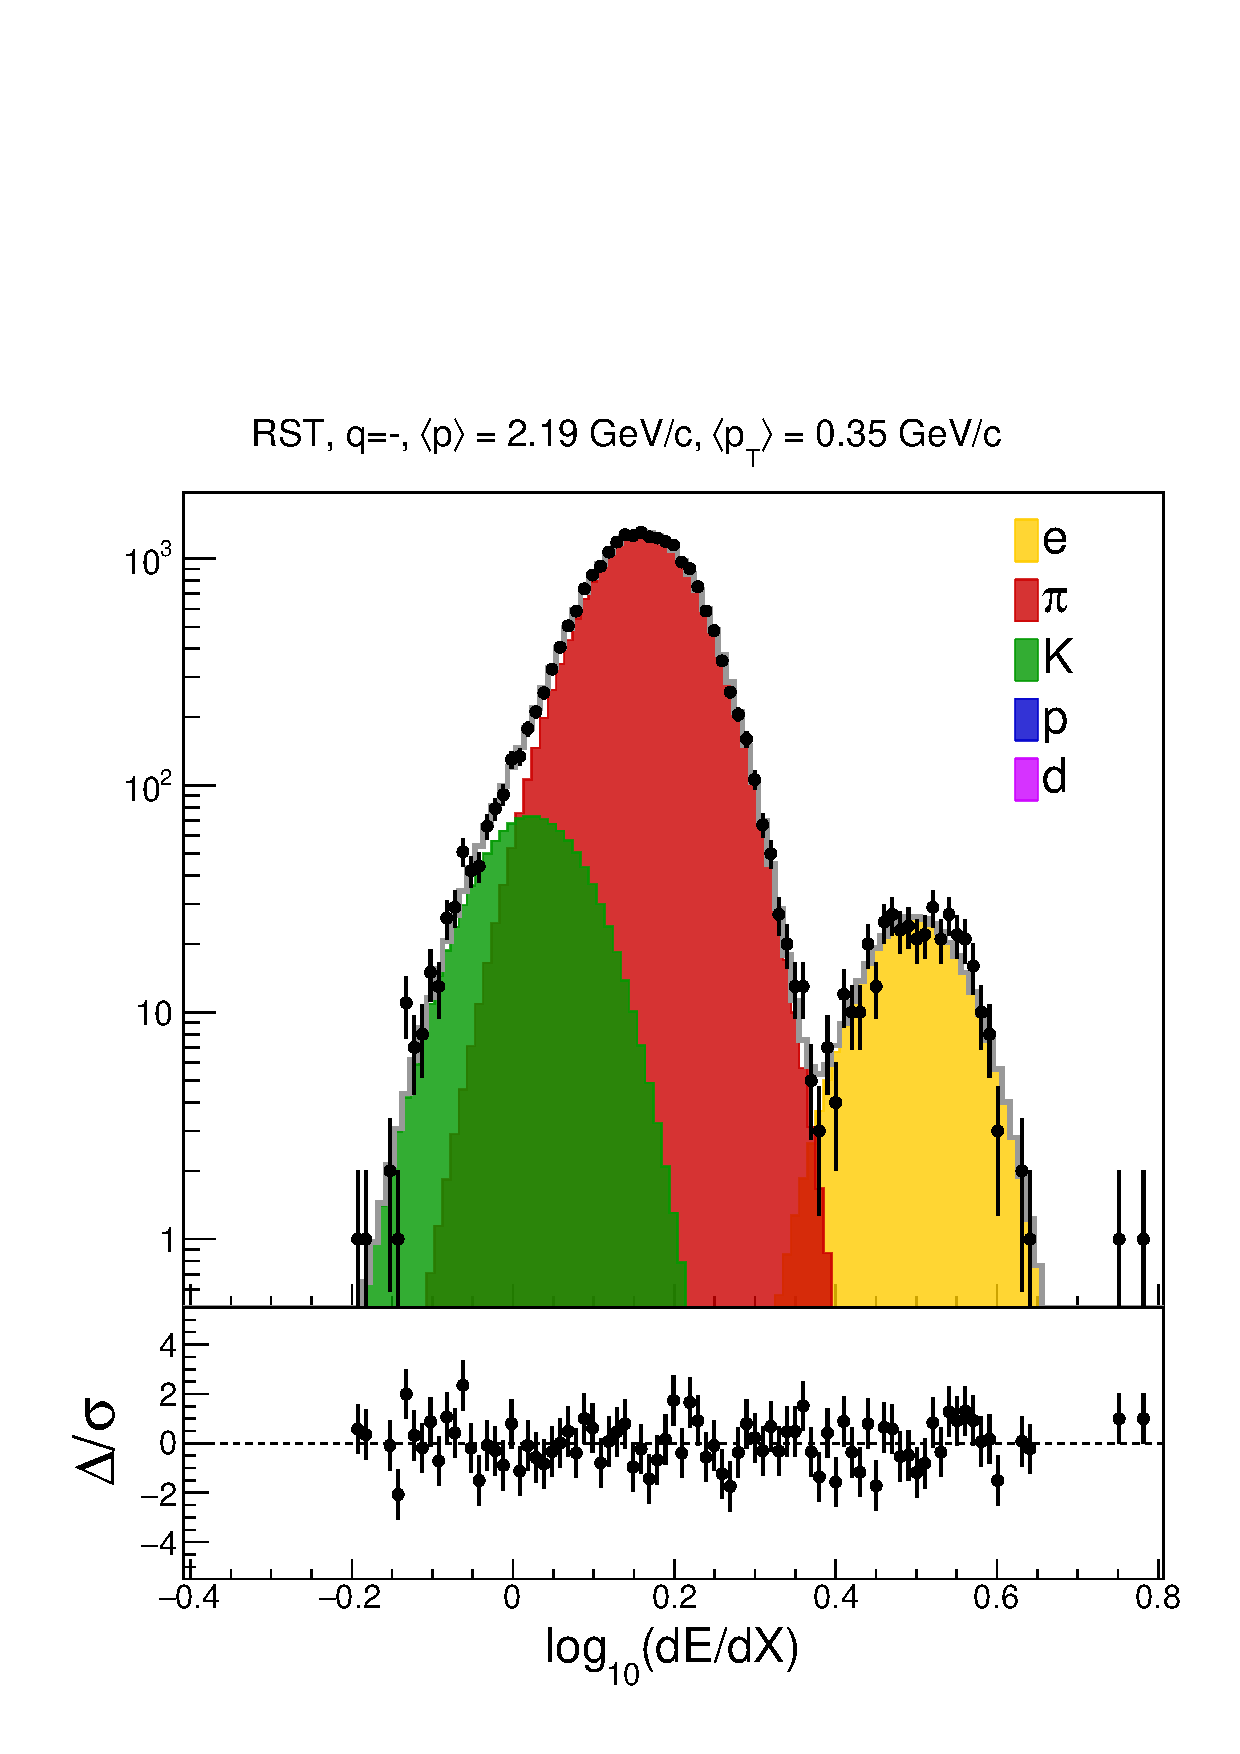
\includegraphics[clip, rviewport=0 0 1 1,width=0.4\textwidth]{dedx/dist_350_v0_c0_x13_y3}
  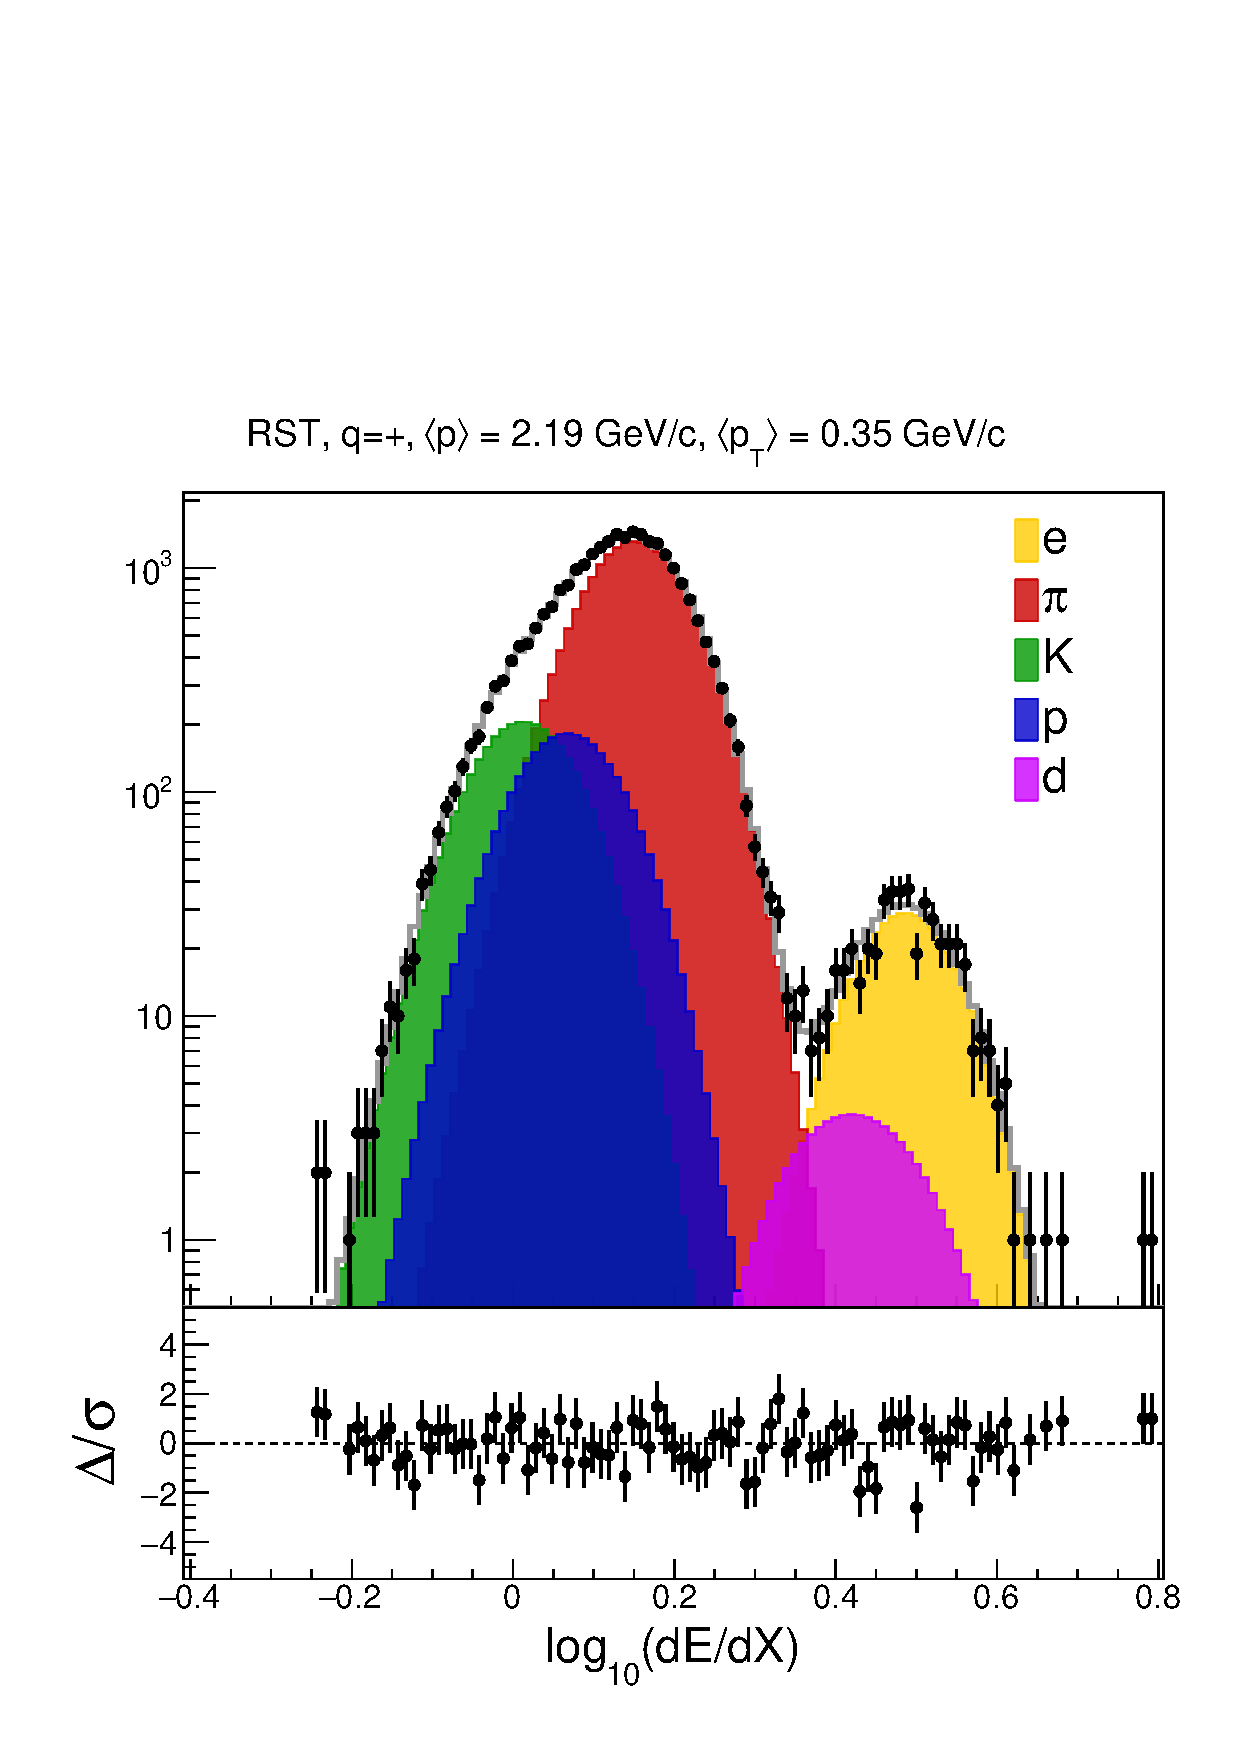
\includegraphics[clip, rviewport=0 0 1 1,width=0.4\textwidth]{dedx/dist_350_v0_c1_x13_y3}

  \vspace{0.5cm}
  
  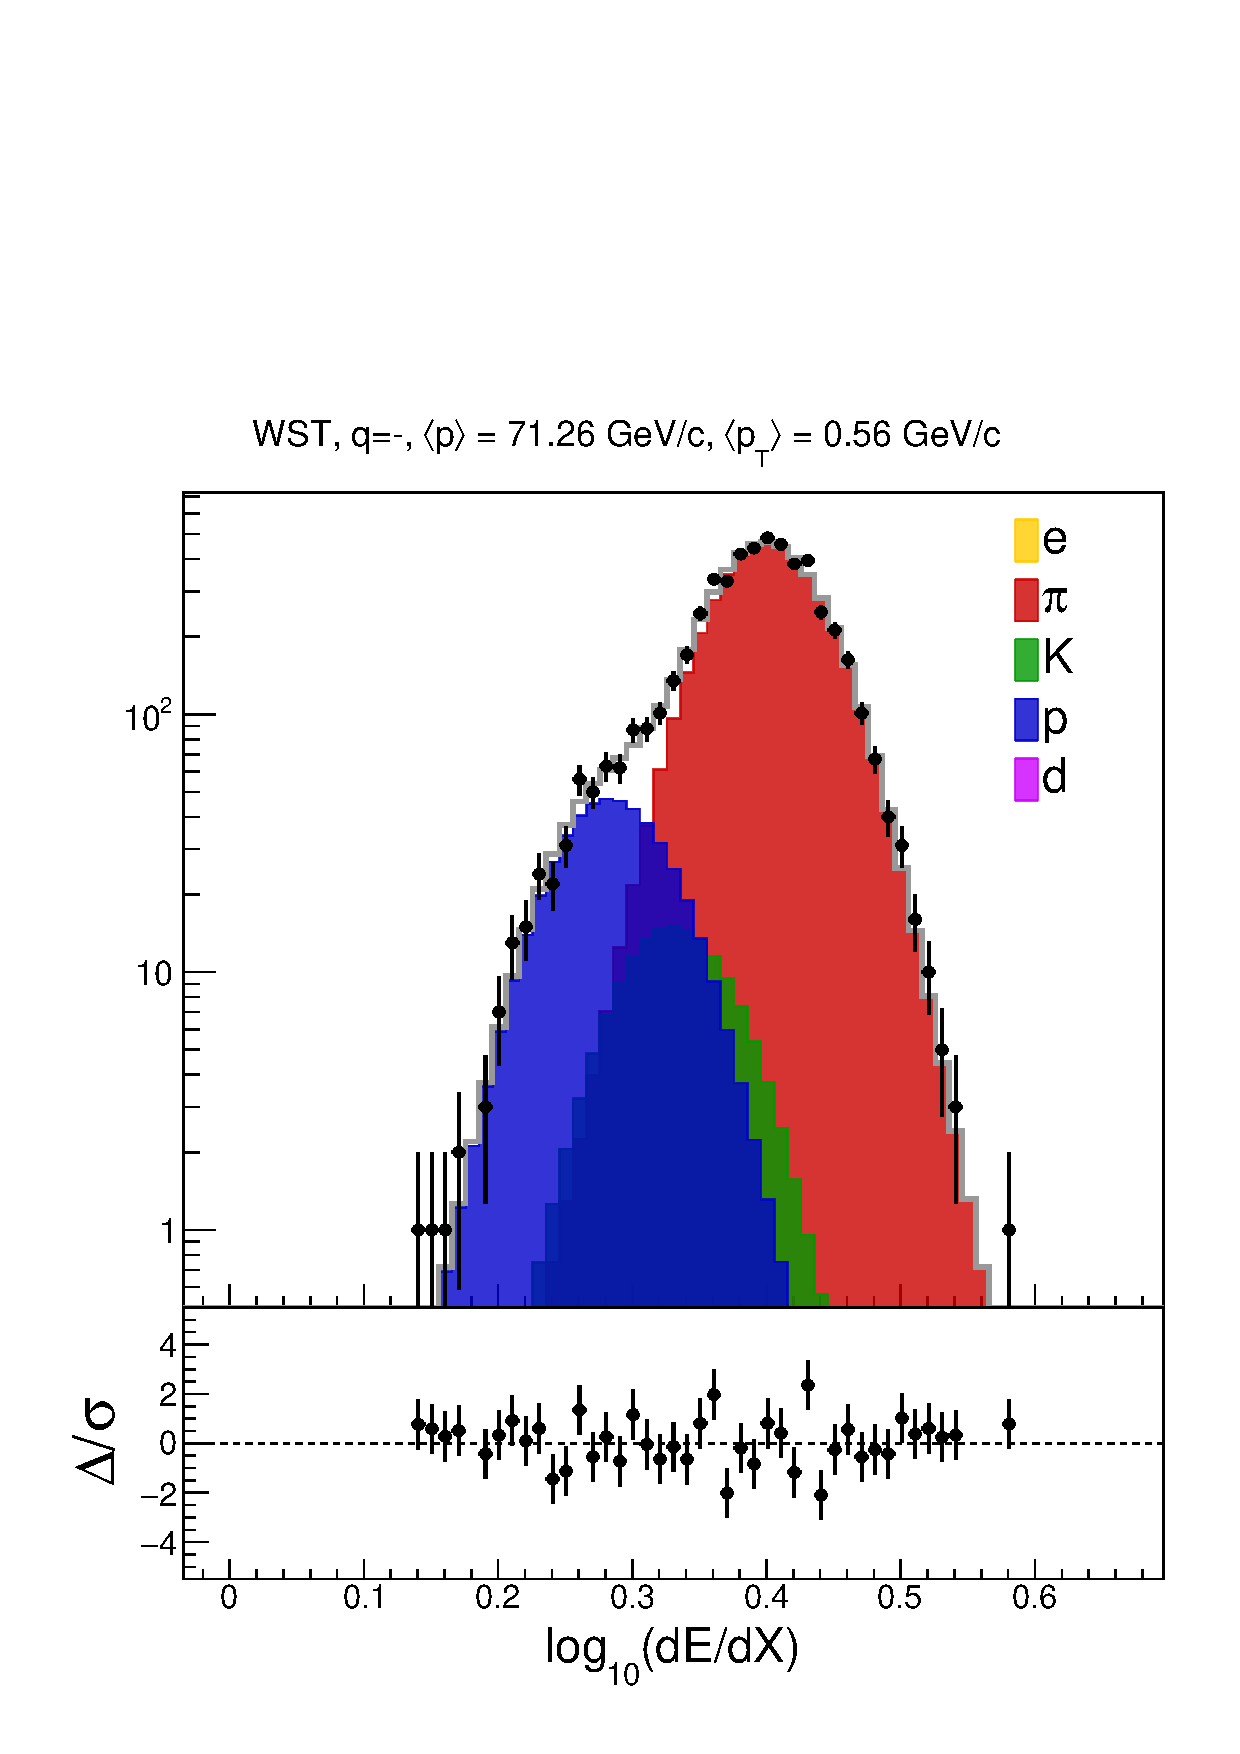
\includegraphics[clip, rviewport=0 0 1 1,width=0.4\textwidth]{dedx/dist_350_v1_c0_x29_y5}
  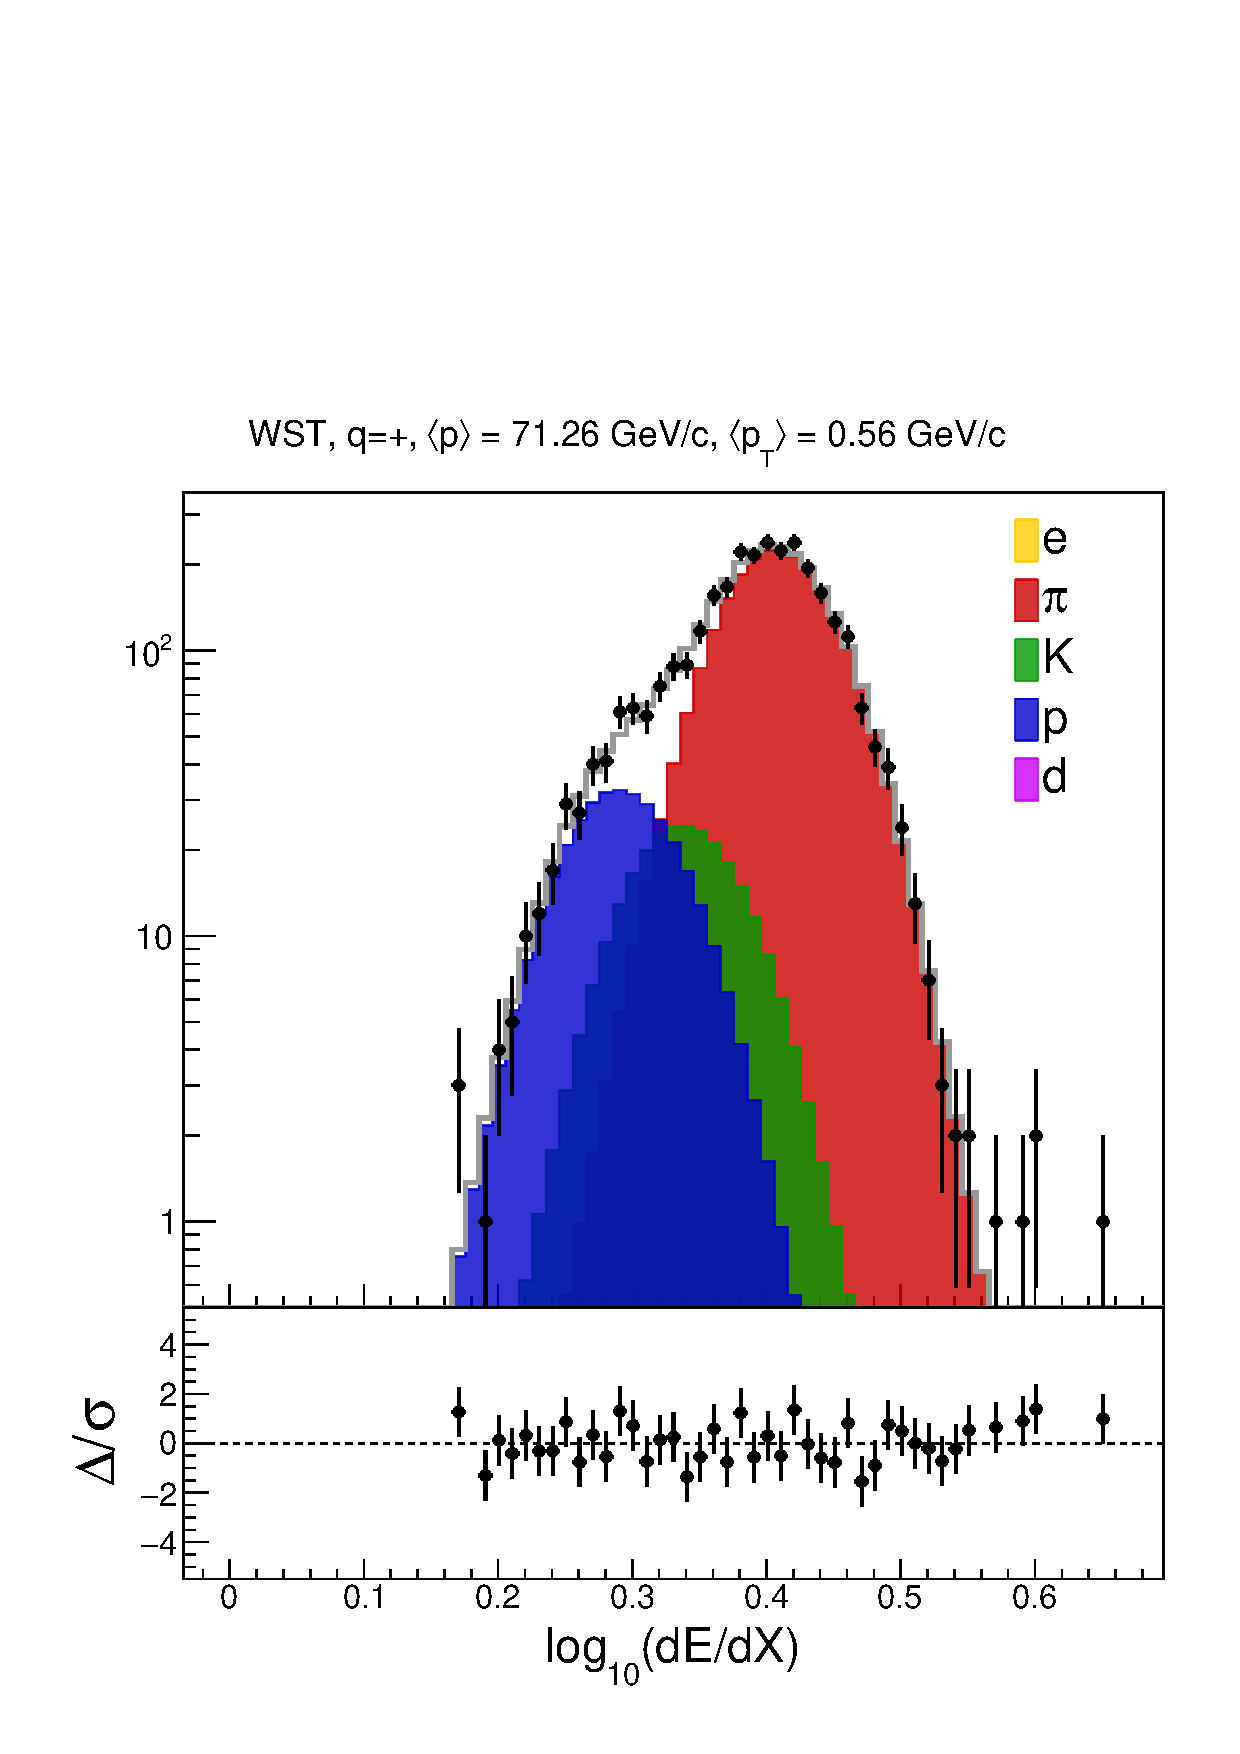
\includegraphics[clip, rviewport=0 0 1 1,width=0.4\textwidth]{dedx/dist_350_v1_c1_x29_y5}
  
  \caption{Examples of the fitted \dedx distributions from the 350 \GeVc dataset.}
  \label{fig:hadron:dedx:fit:dist350}
\end{figure}

%%%%%%%%%% CAL %%%%%%%%%%%%%%
\begin{figure}
  \centering
  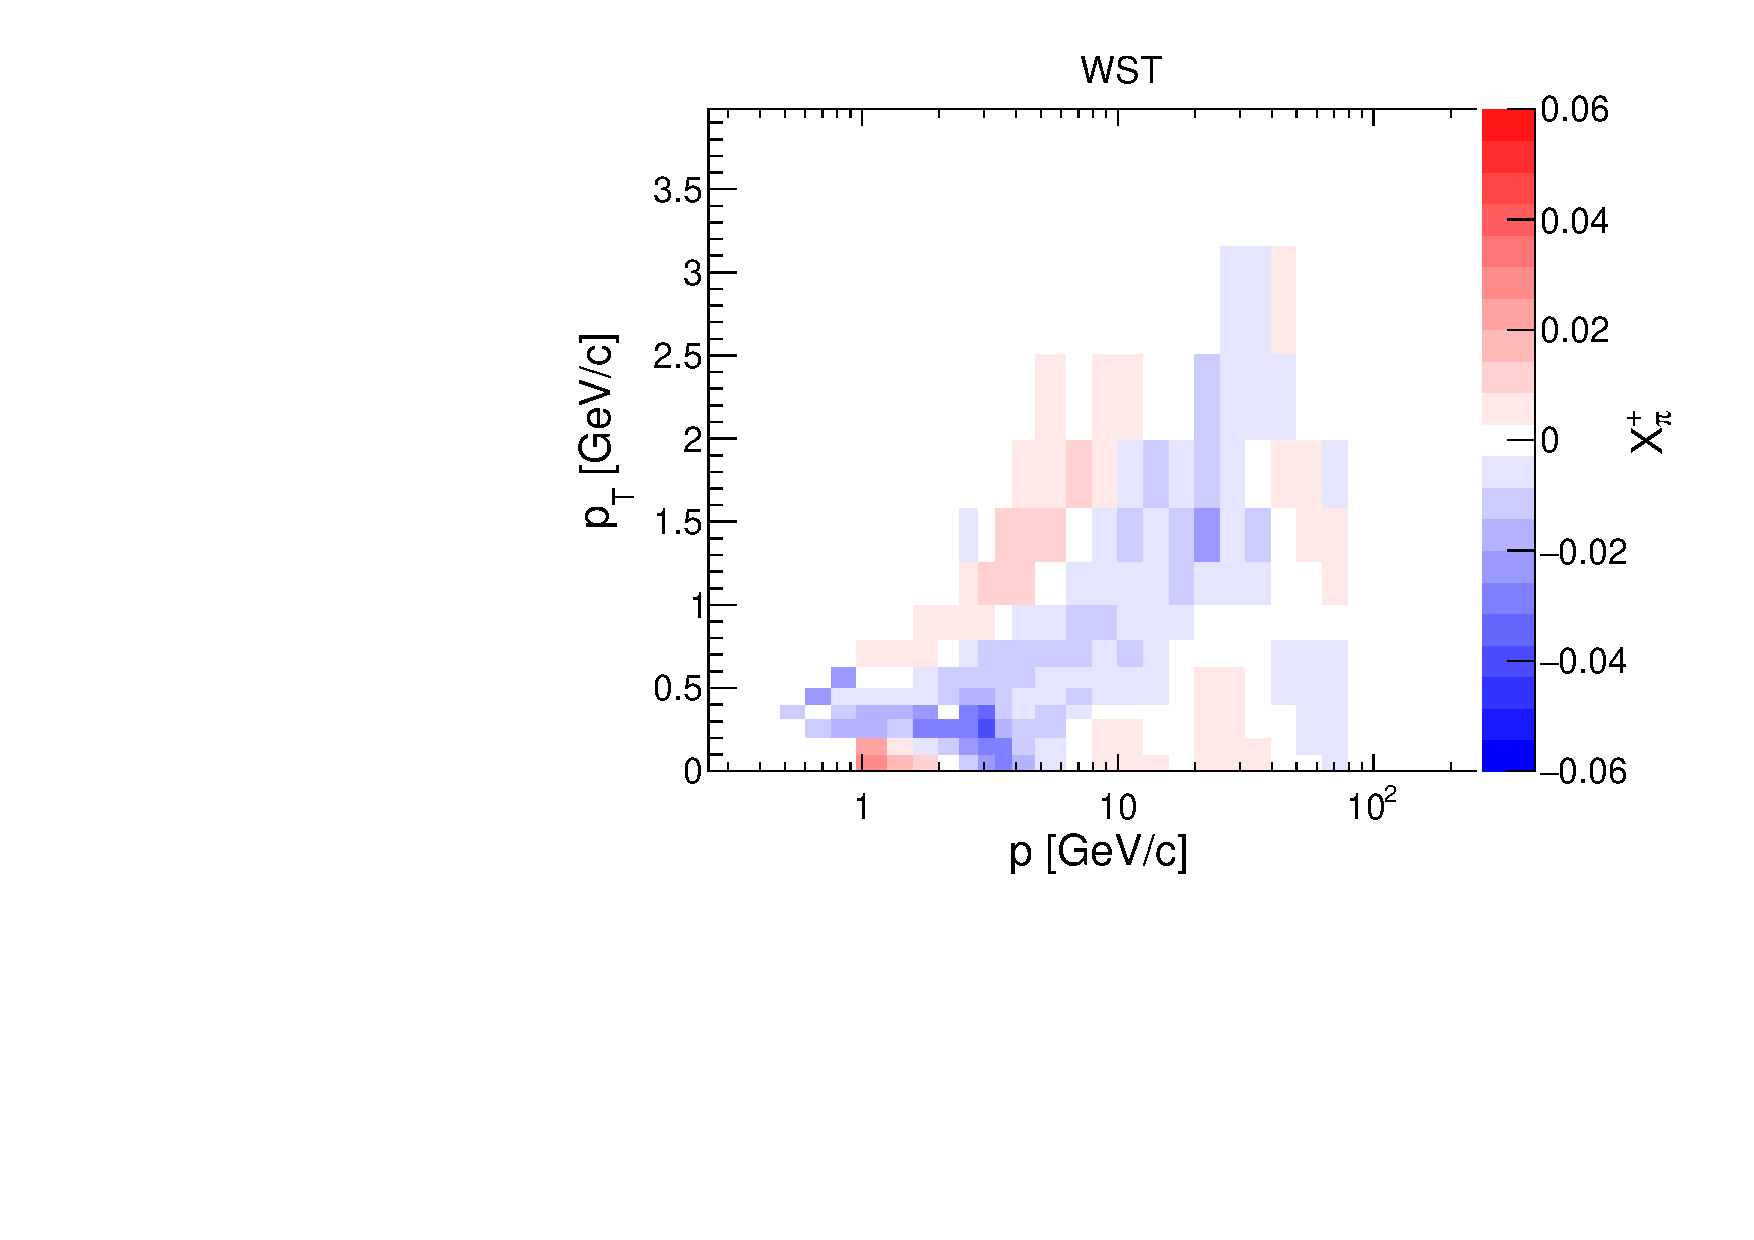
\includegraphics[clip, rviewport=0 0 1 0.94,width=0.4\textwidth]{dedx/model_158_v1_m0}
  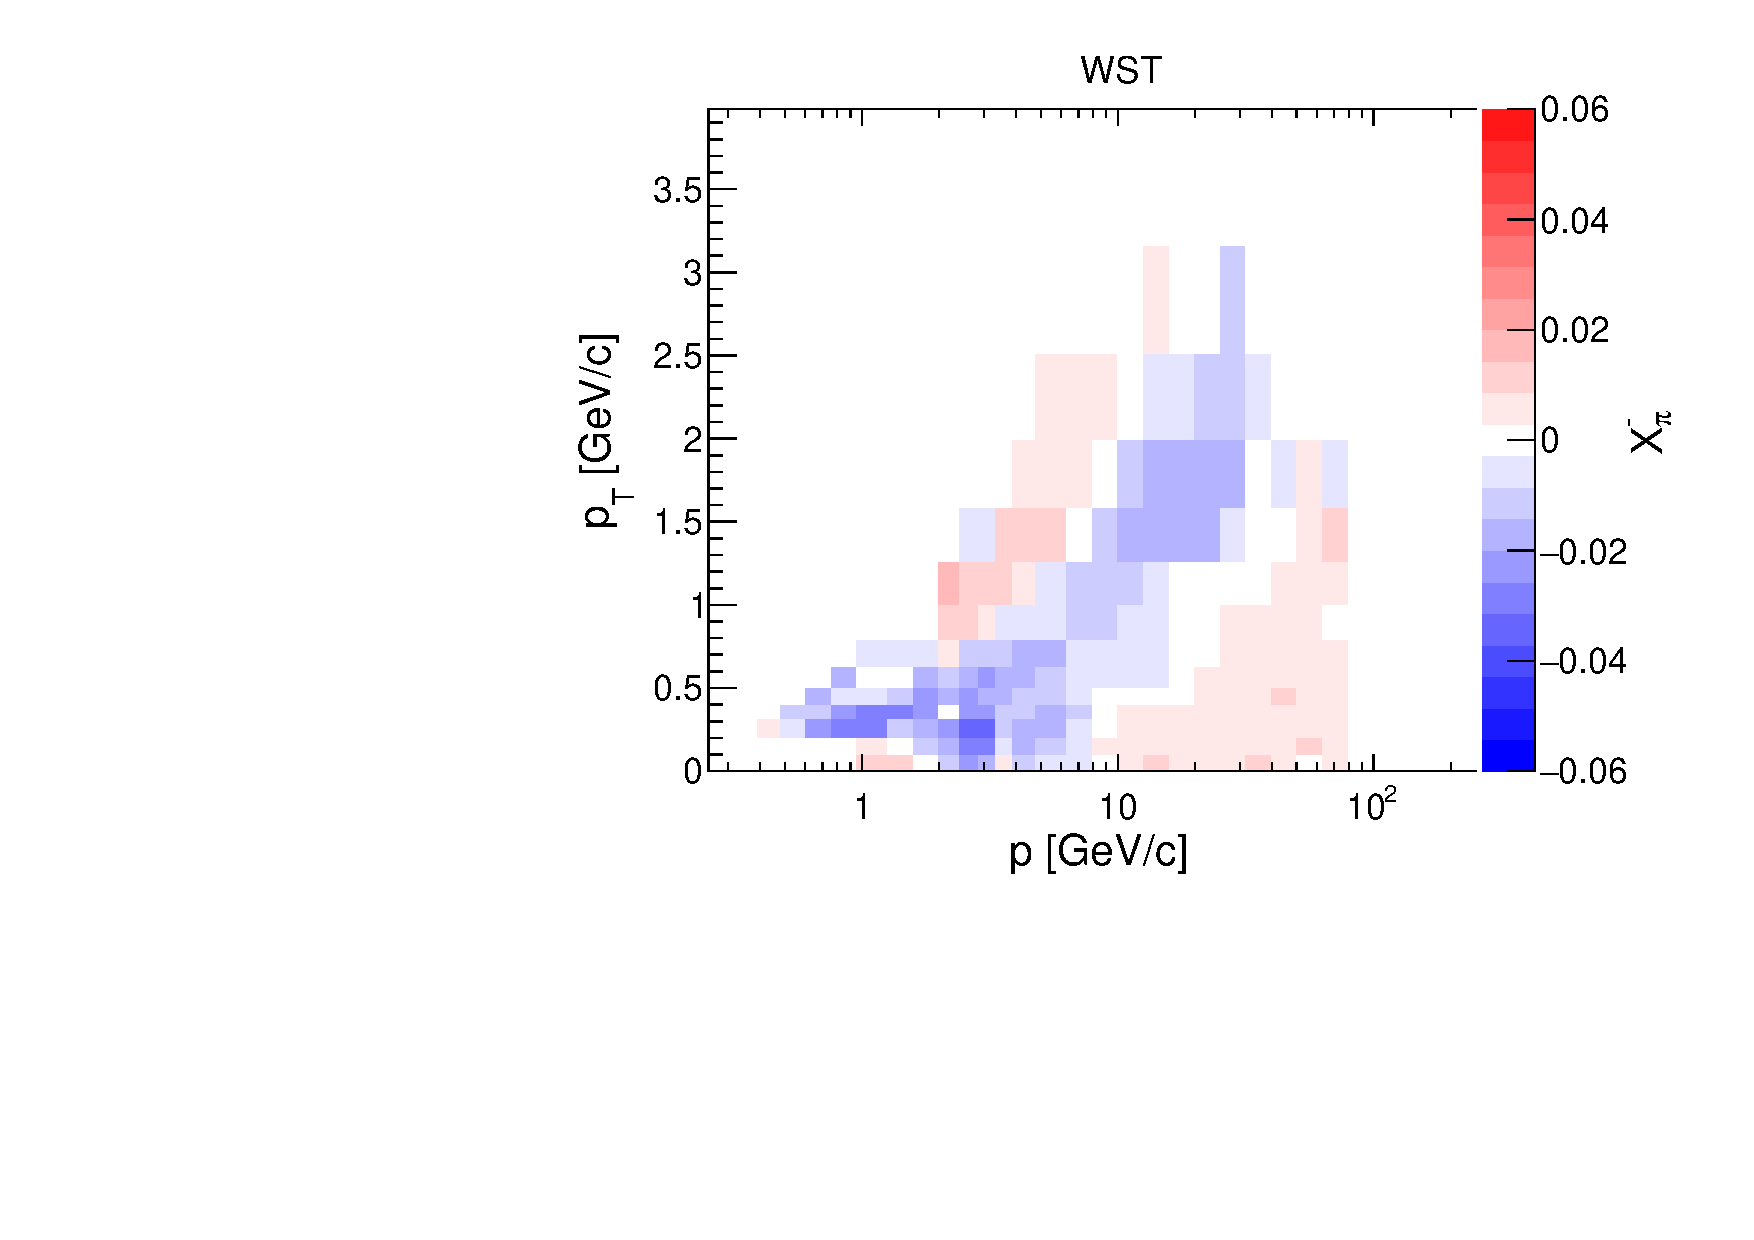
\includegraphics[clip, rviewport=0 0 1 0.94,width=0.4\textwidth]{dedx/model_158_v1_m1}

  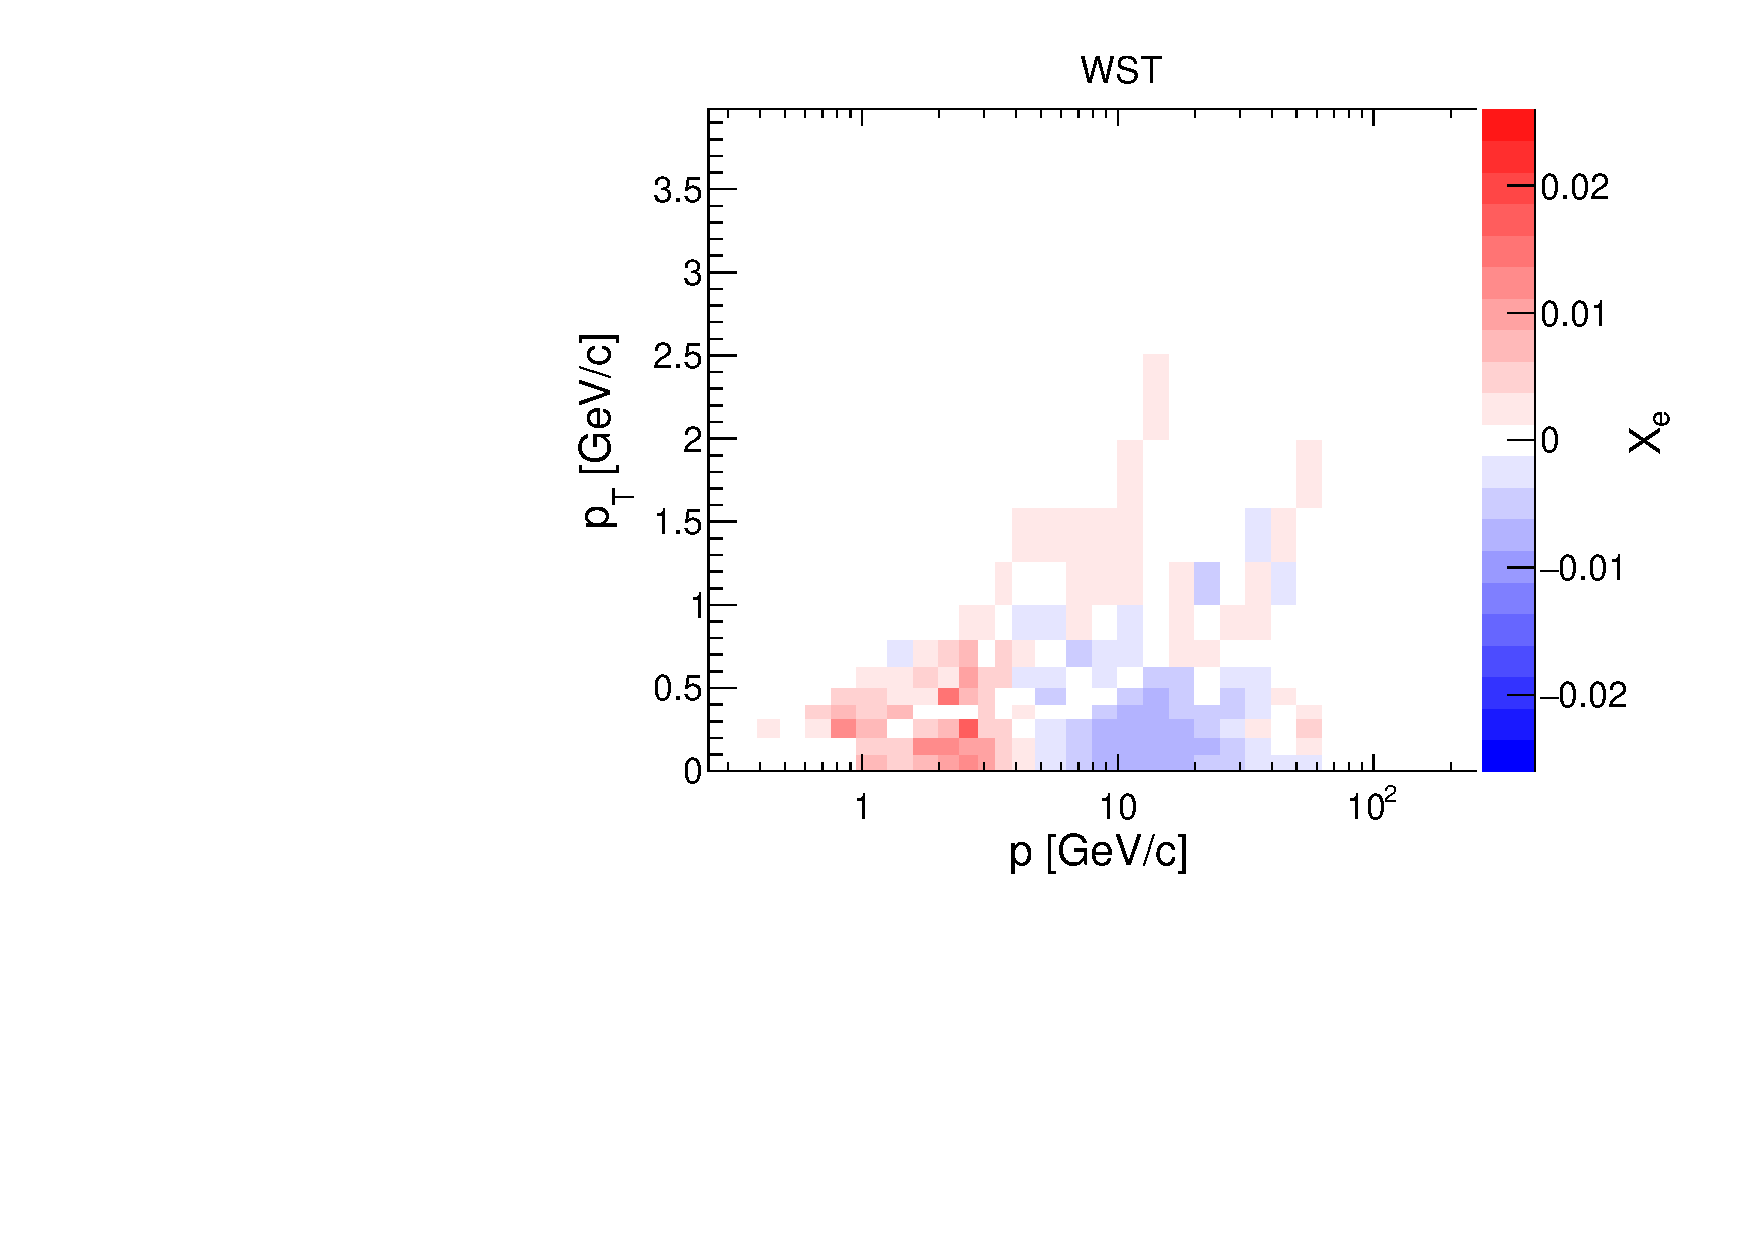
\includegraphics[clip, rviewport=0 0 1 0.94,width=0.4\textwidth]{dedx/model_158_v1_m2}
  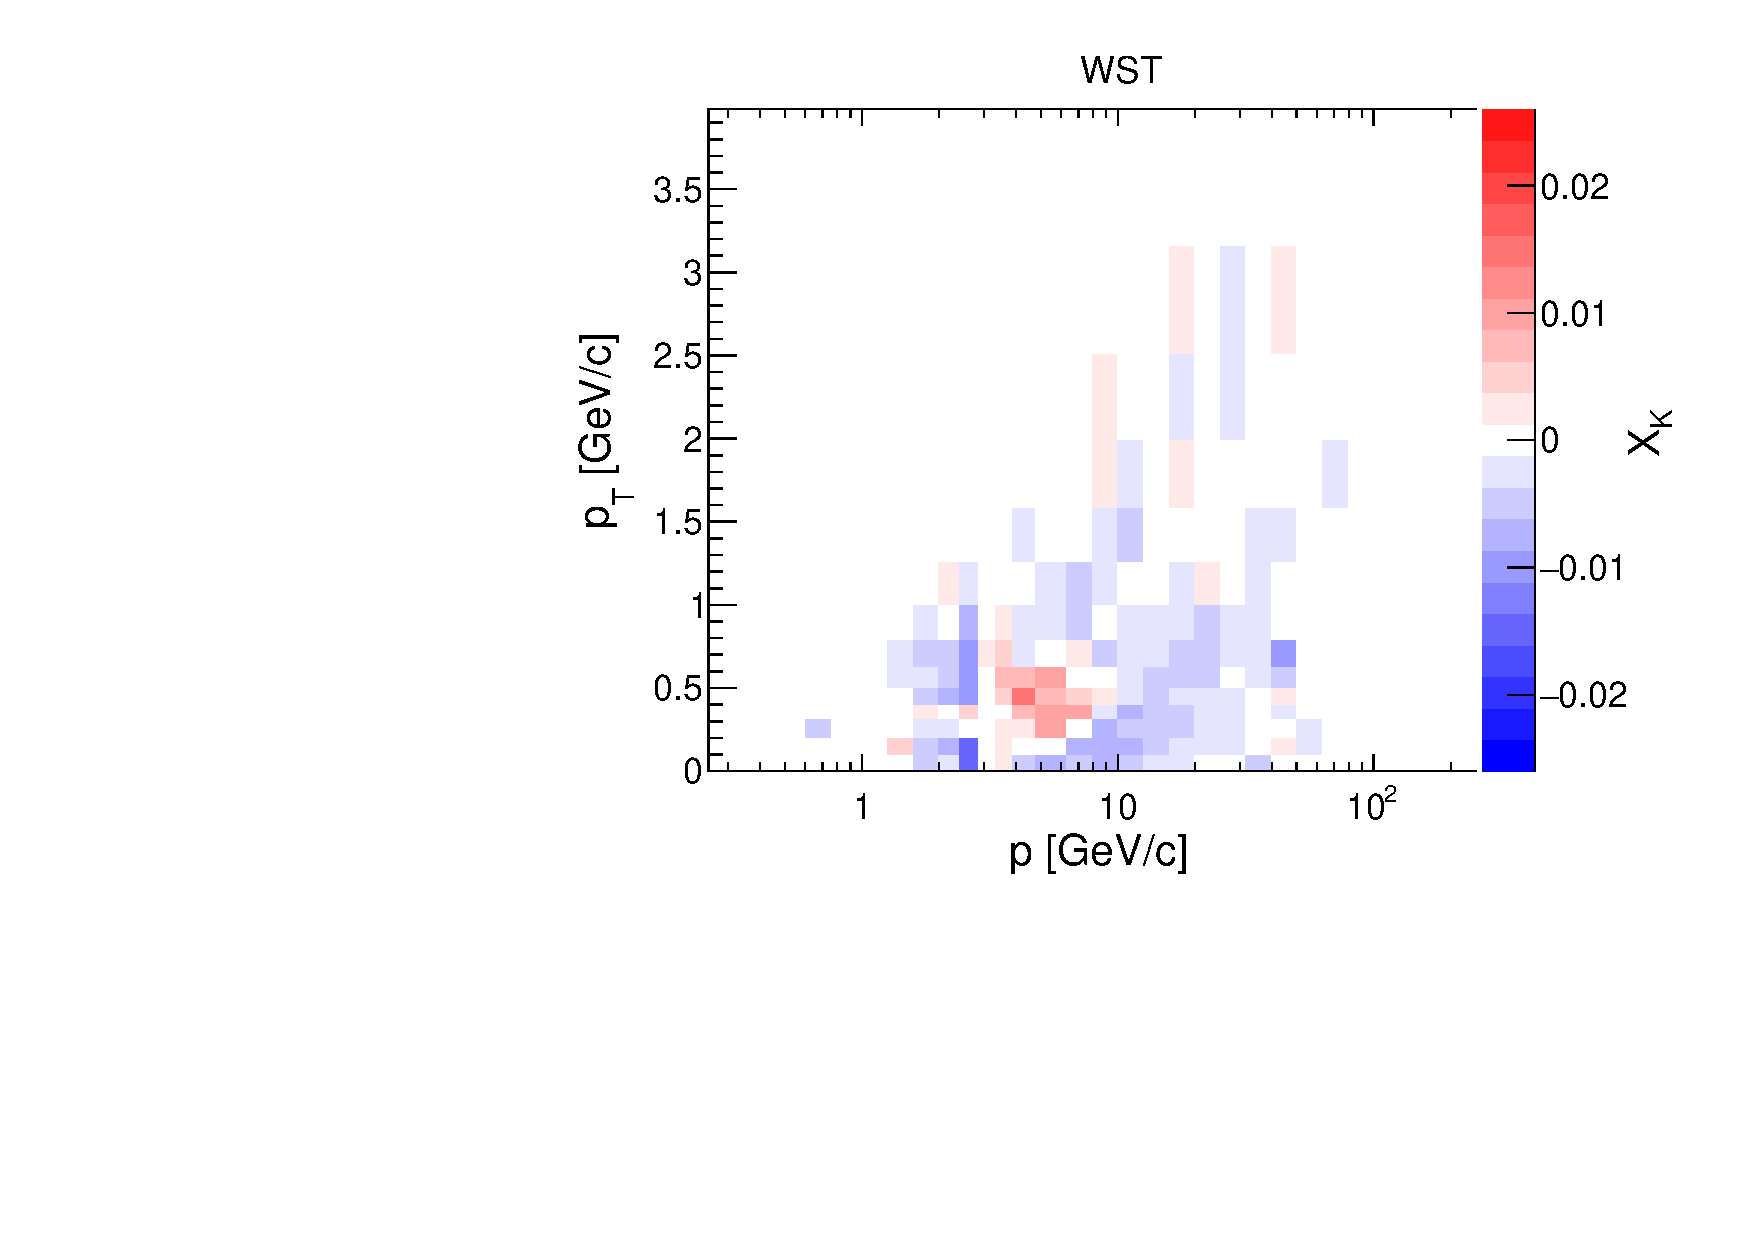
\includegraphics[clip, rviewport=0 0 1 0.94,width=0.4\textwidth]{dedx/model_158_v1_m3}

  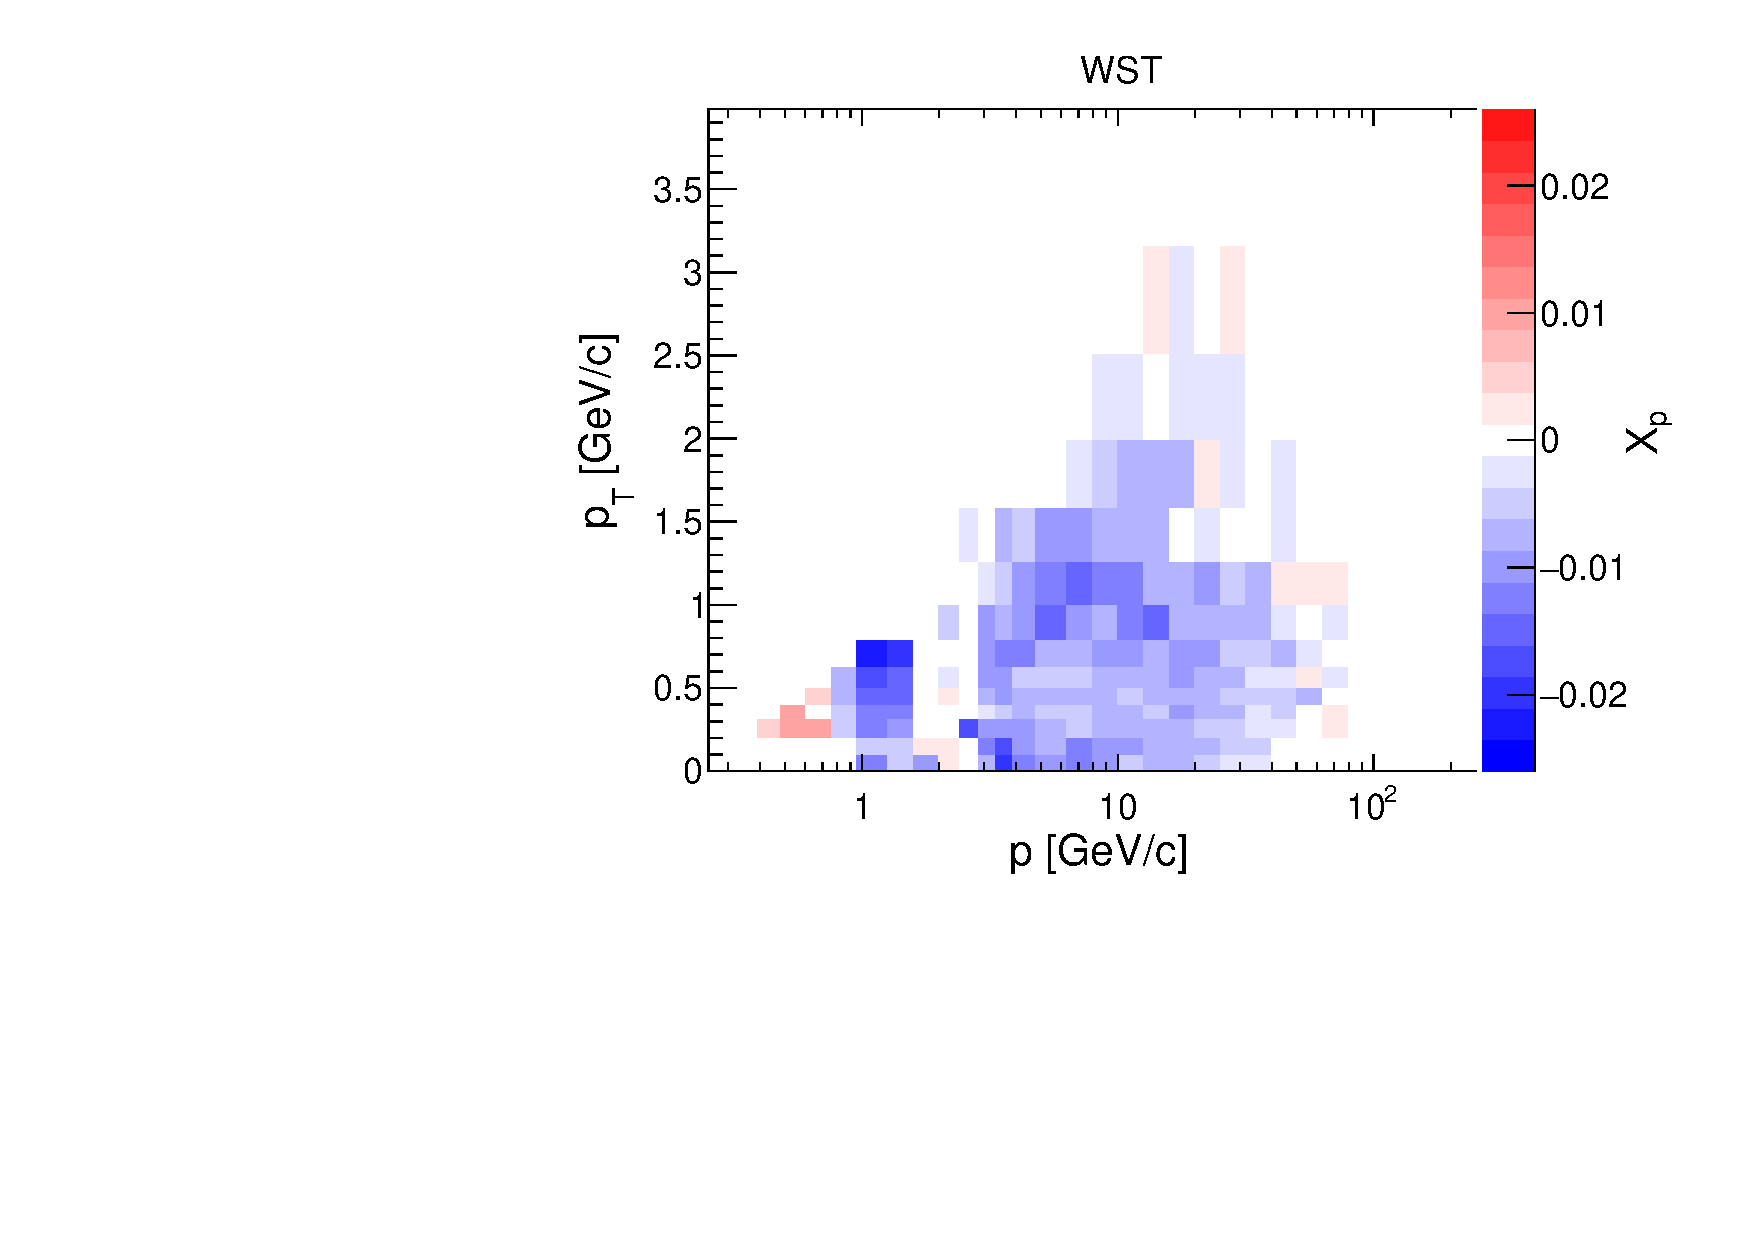
\includegraphics[clip, rviewport=0 0 1 0.94,width=0.4\textwidth]{dedx/model_158_v1_m4}
  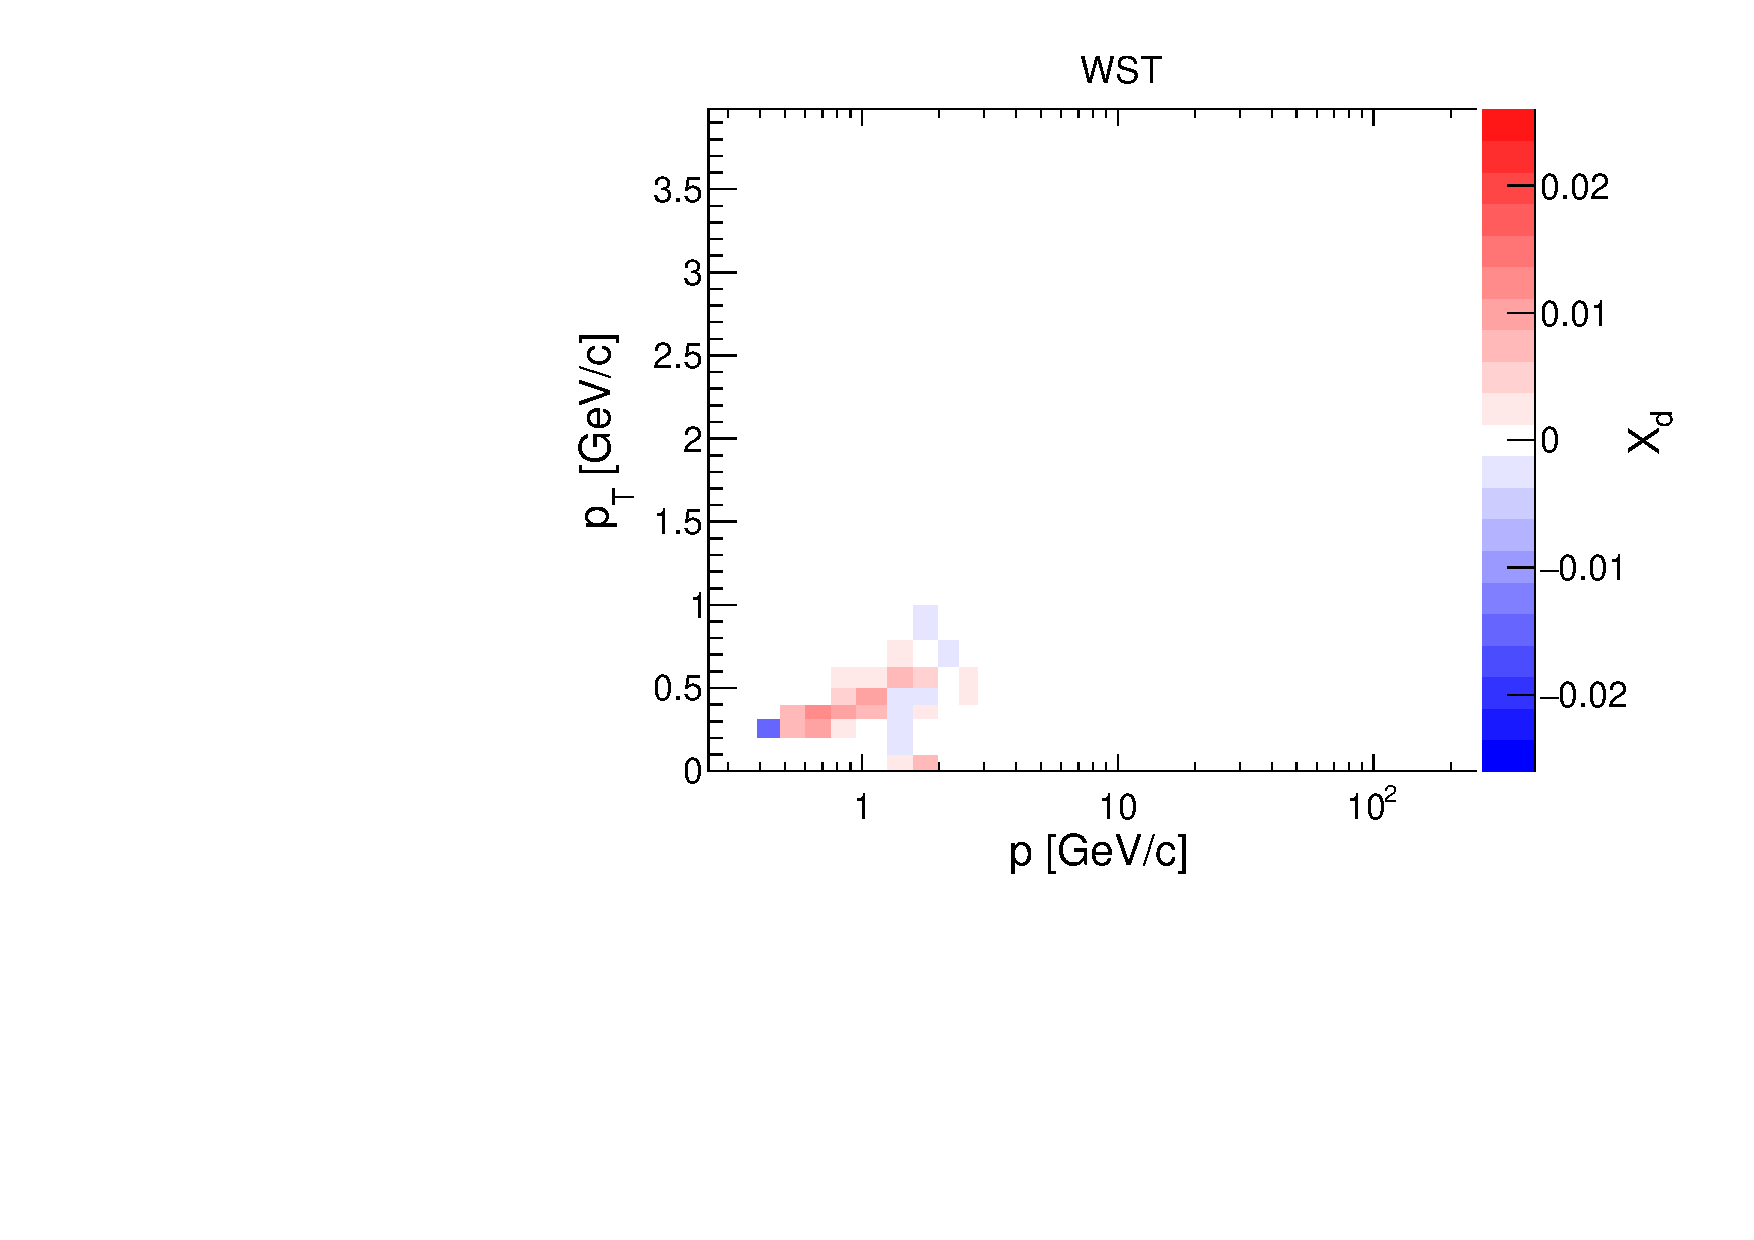
\includegraphics[clip, rviewport=0 0 1 0.94,width=0.4\textwidth]{dedx/model_158_v1_m5}
  \caption{Calibration constants obtained from the fit of the WST dataset at 158 \GeVc.}
  \label{fig:hadron:dedx:fit:cal158w}
\end{figure}

%%%%%%%%%% CAL %%%%%%%%%%%%%%
\begin{figure}
  \centering
  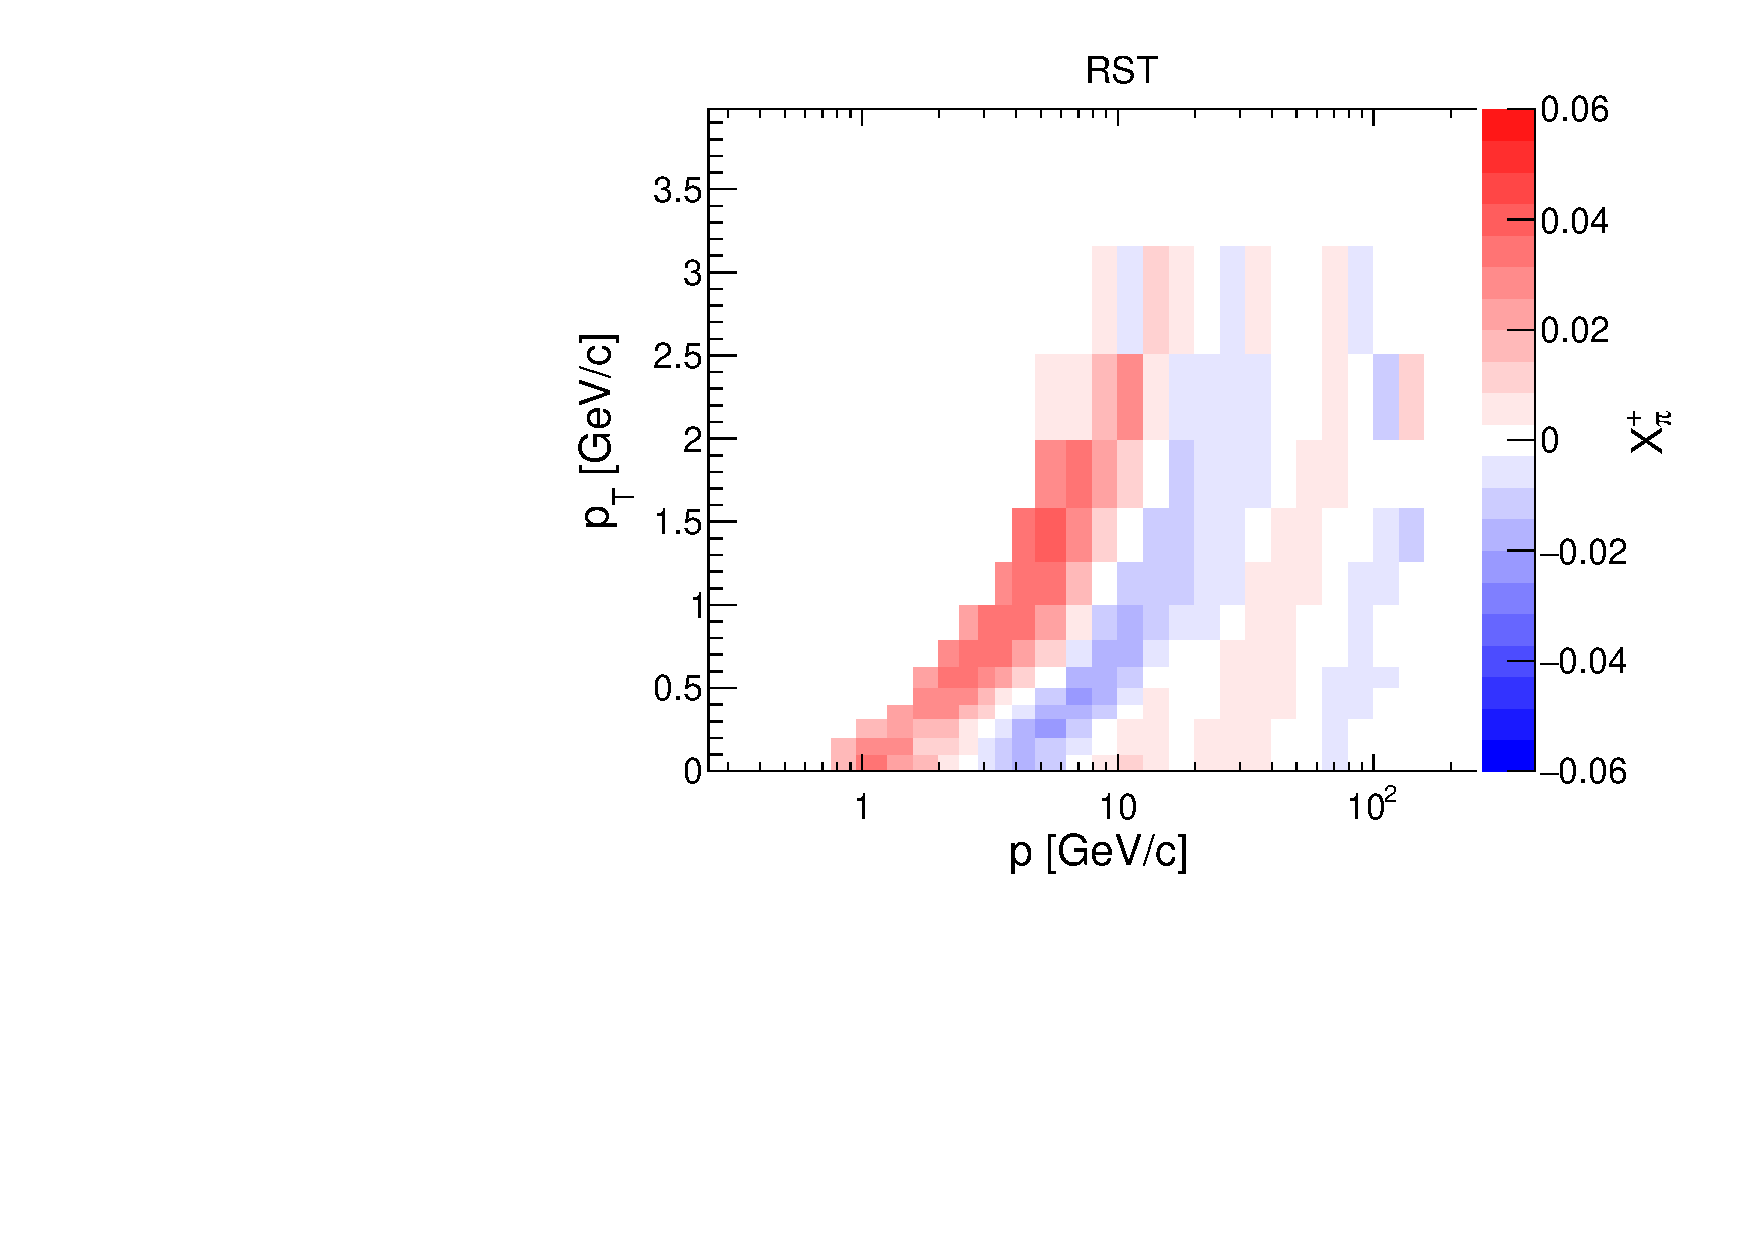
\includegraphics[clip, rviewport=0 0 1 0.94,width=0.4\textwidth]{dedx/model_350_v0_m0}
  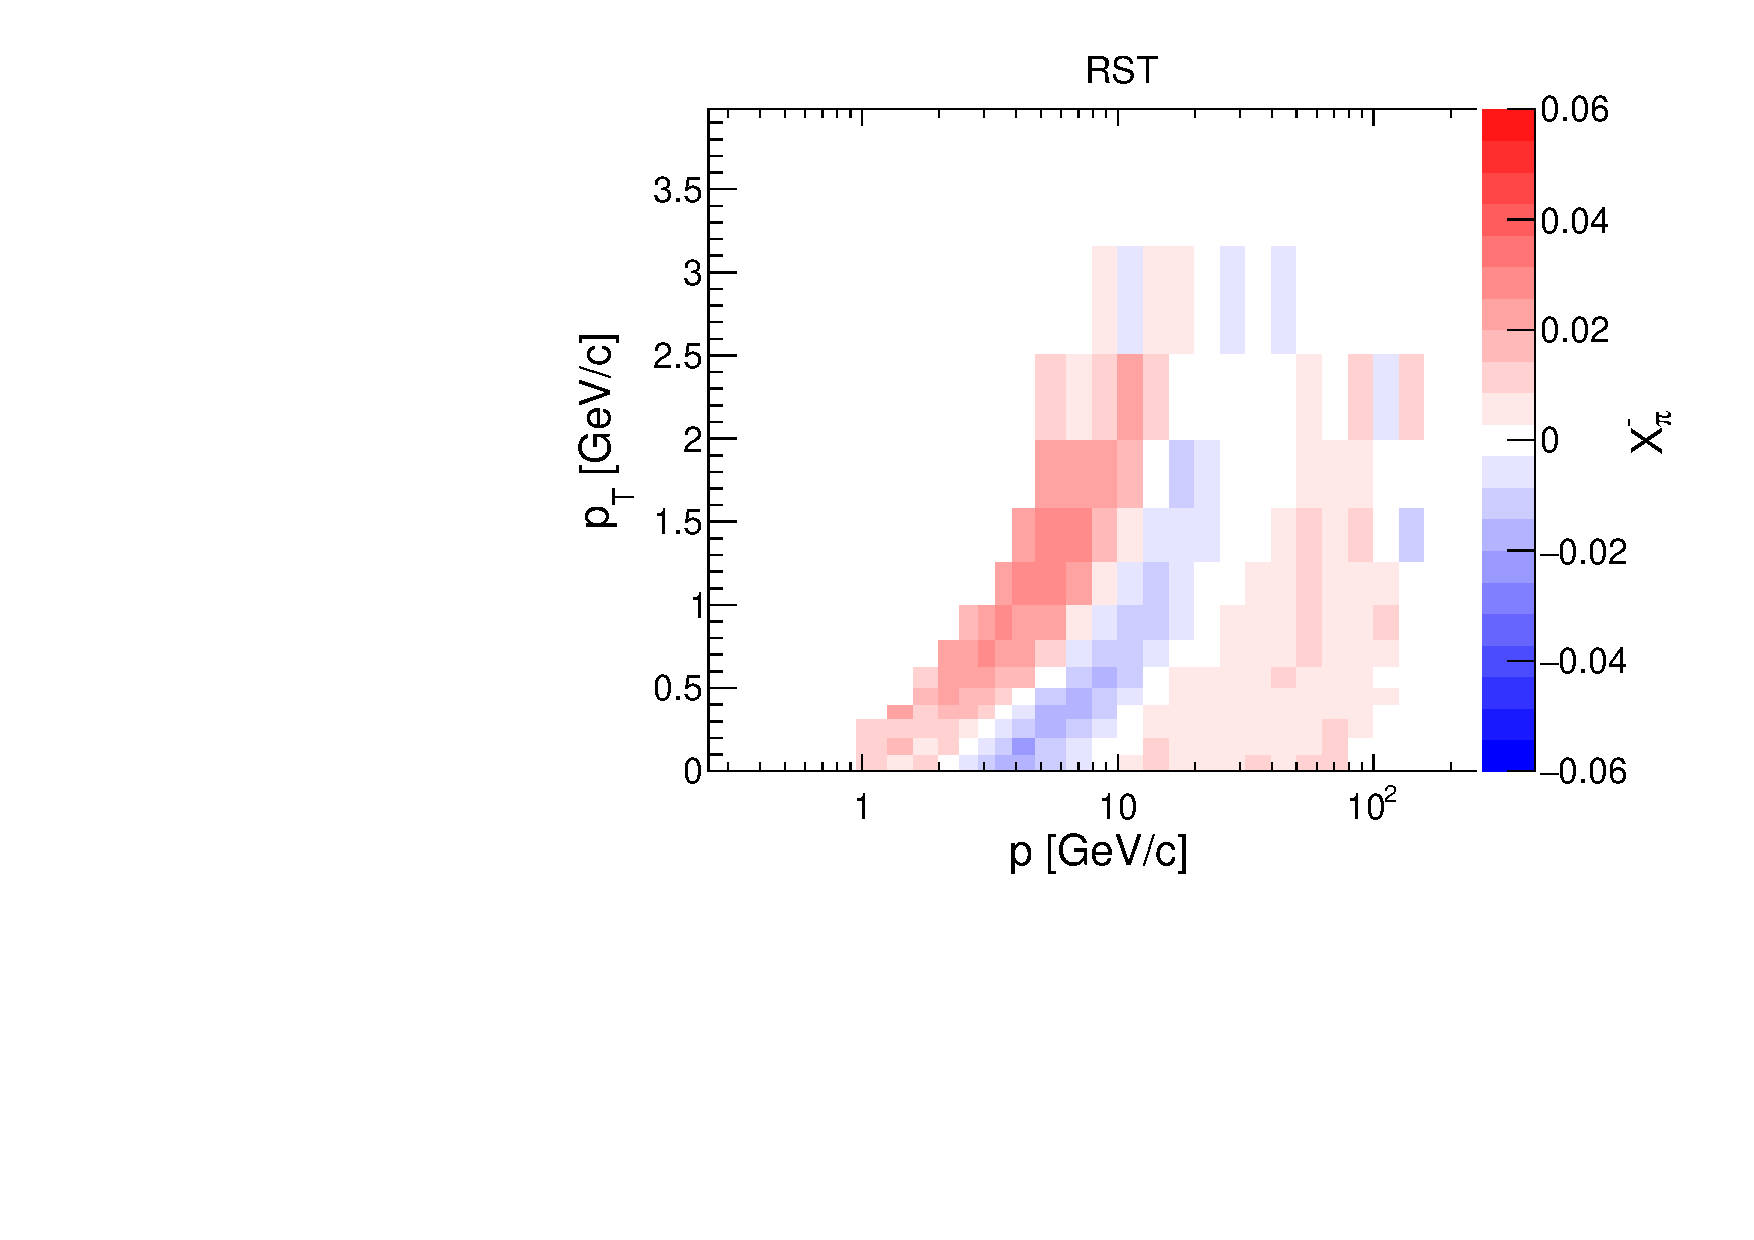
\includegraphics[clip, rviewport=0 0 1 0.94,width=0.4\textwidth]{dedx/model_350_v0_m1}

  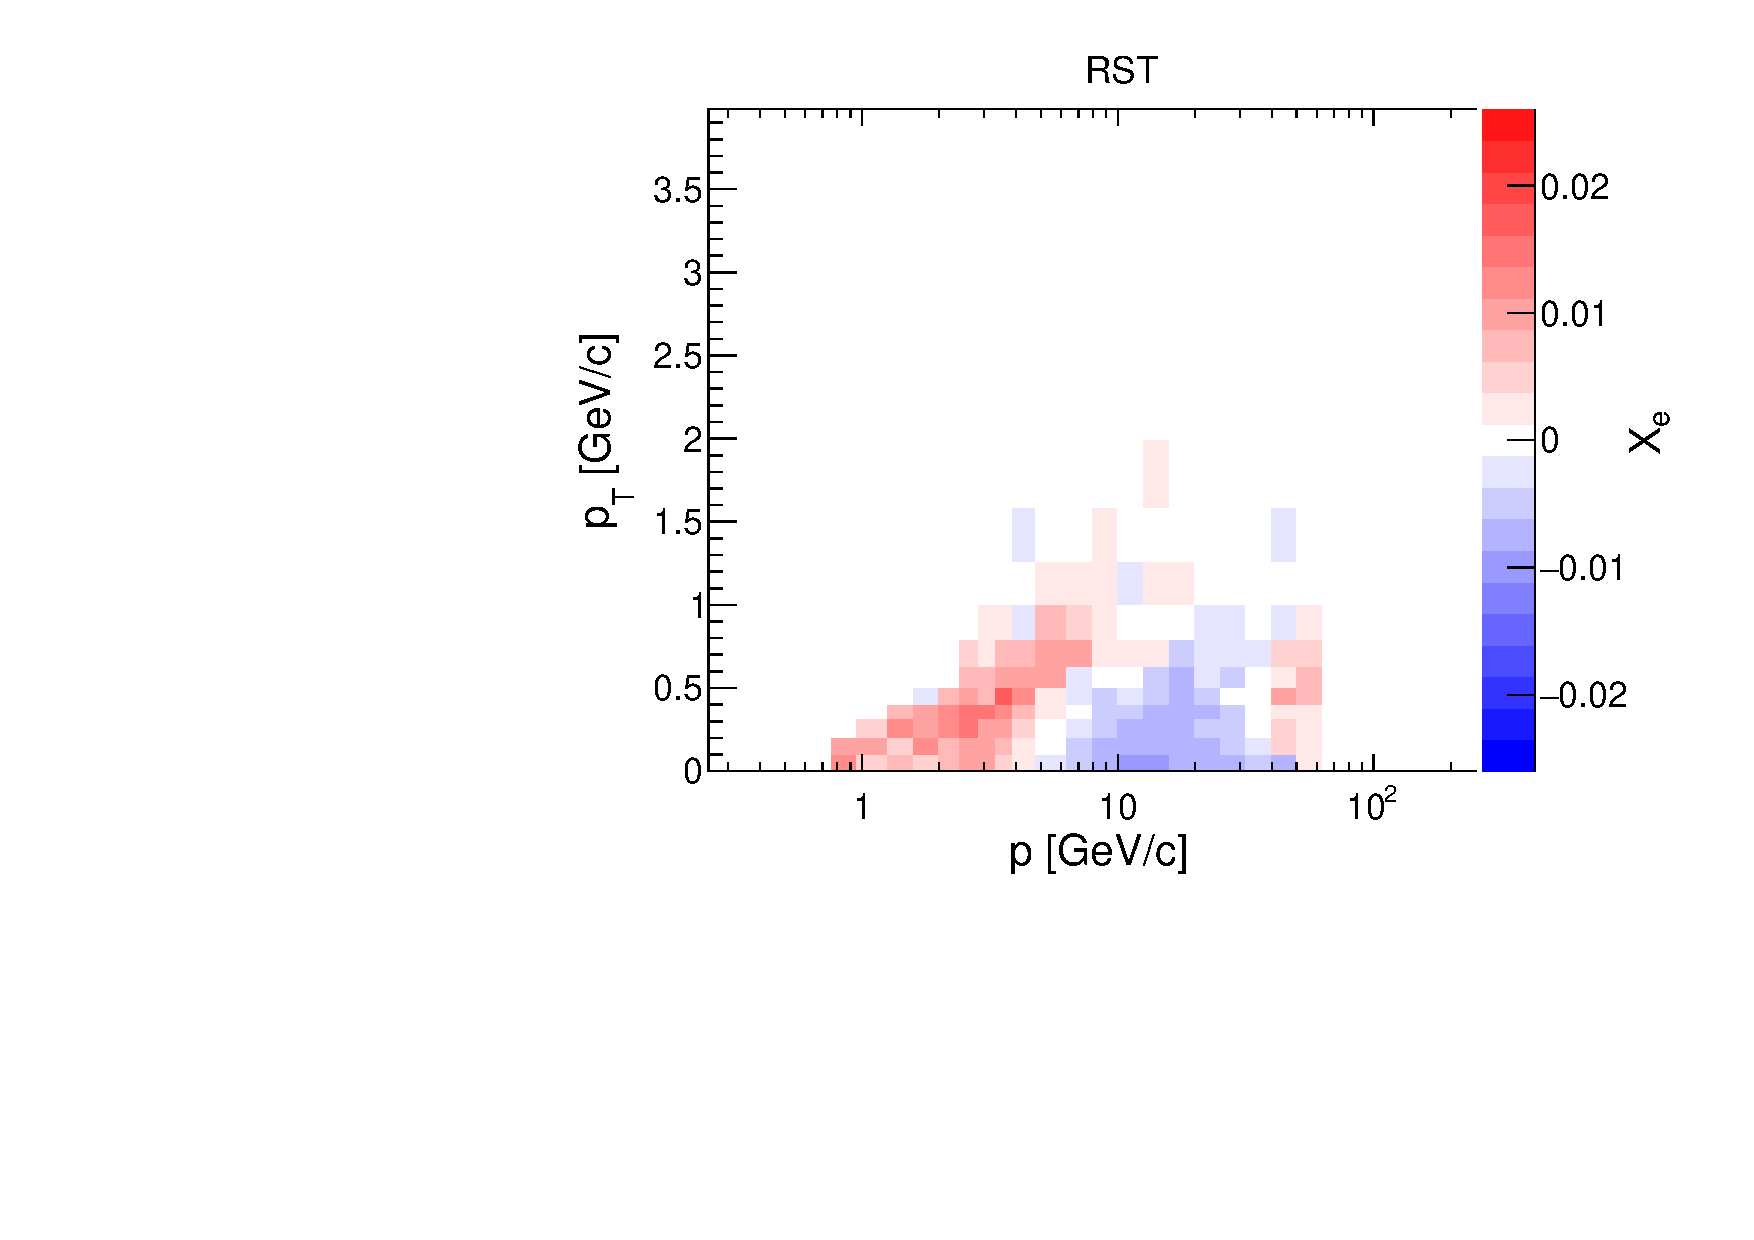
\includegraphics[clip, rviewport=0 0 1 0.94,width=0.4\textwidth]{dedx/model_350_v0_m2}
  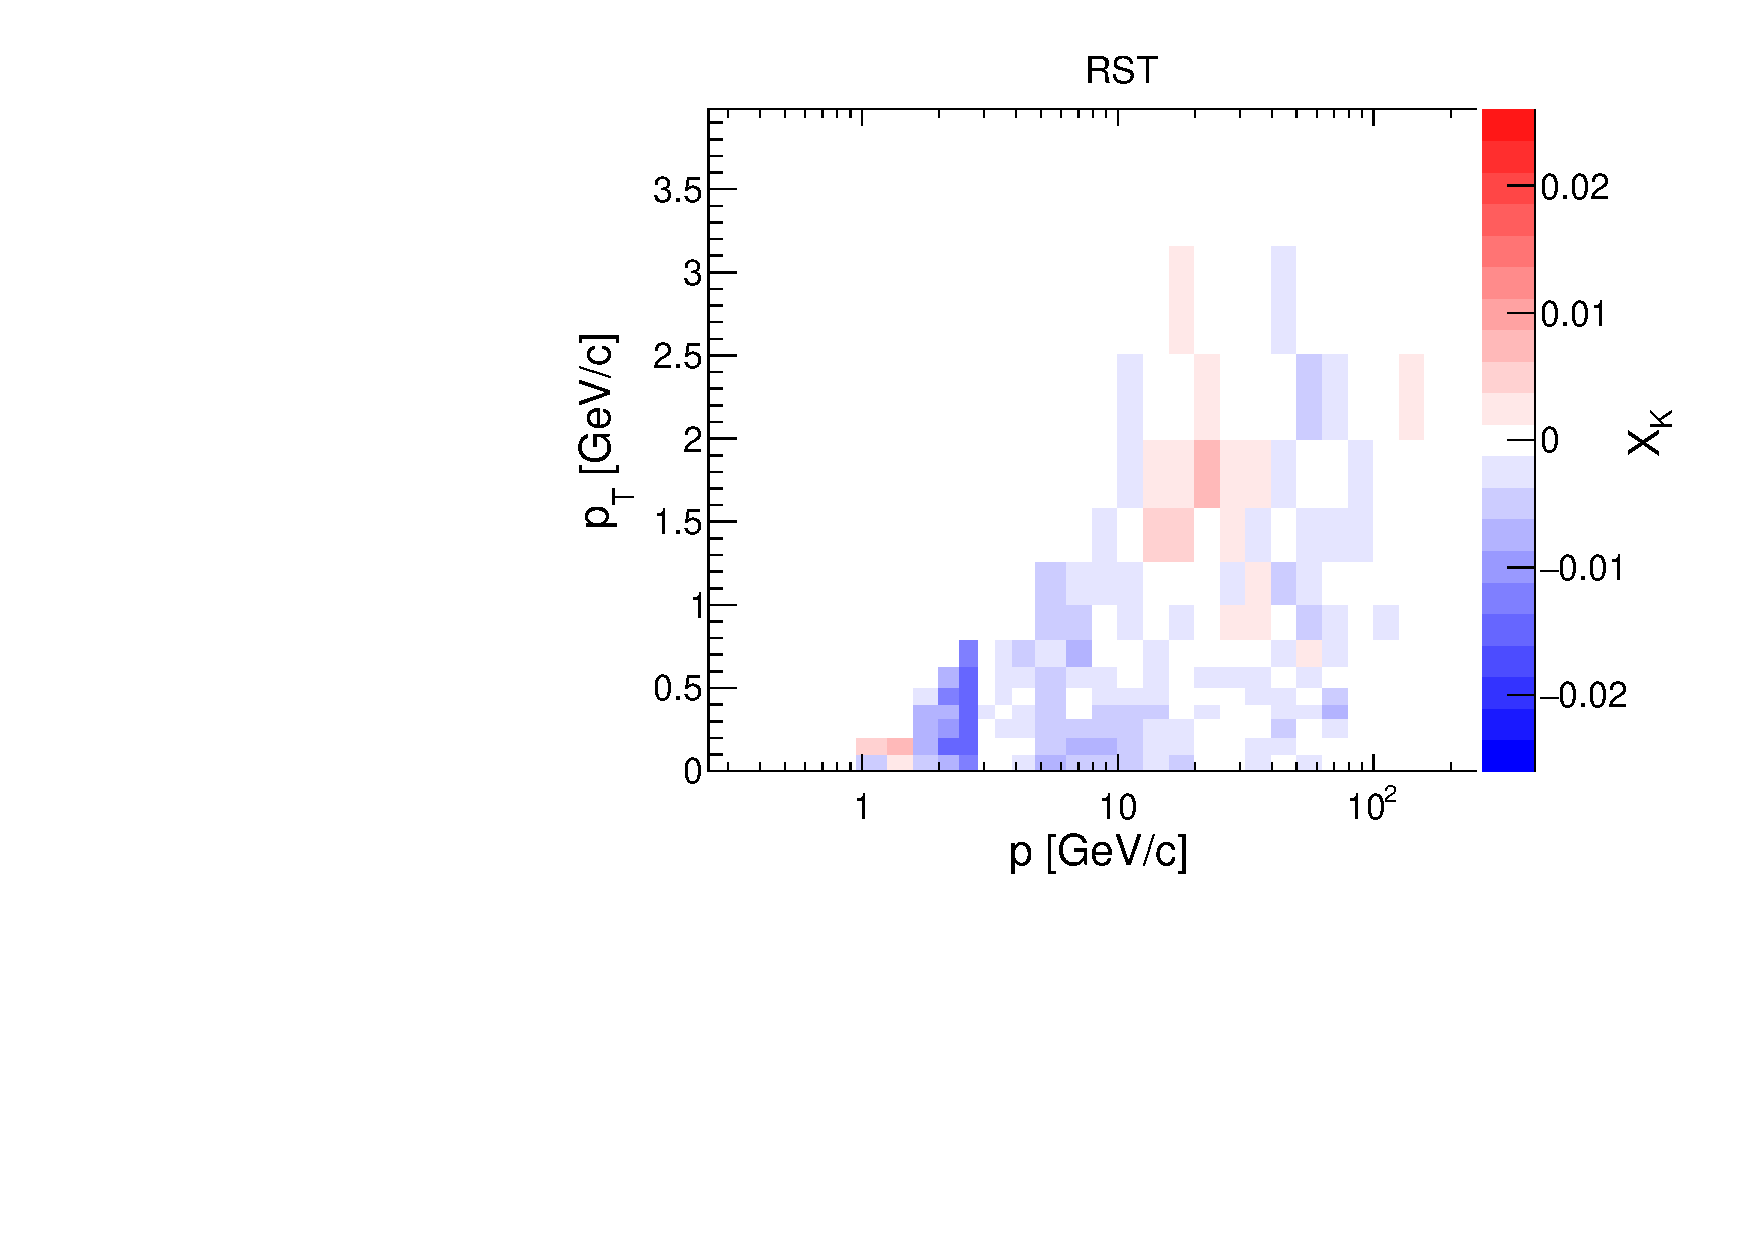
\includegraphics[clip, rviewport=0 0 1 0.94,width=0.4\textwidth]{dedx/model_350_v0_m3}

  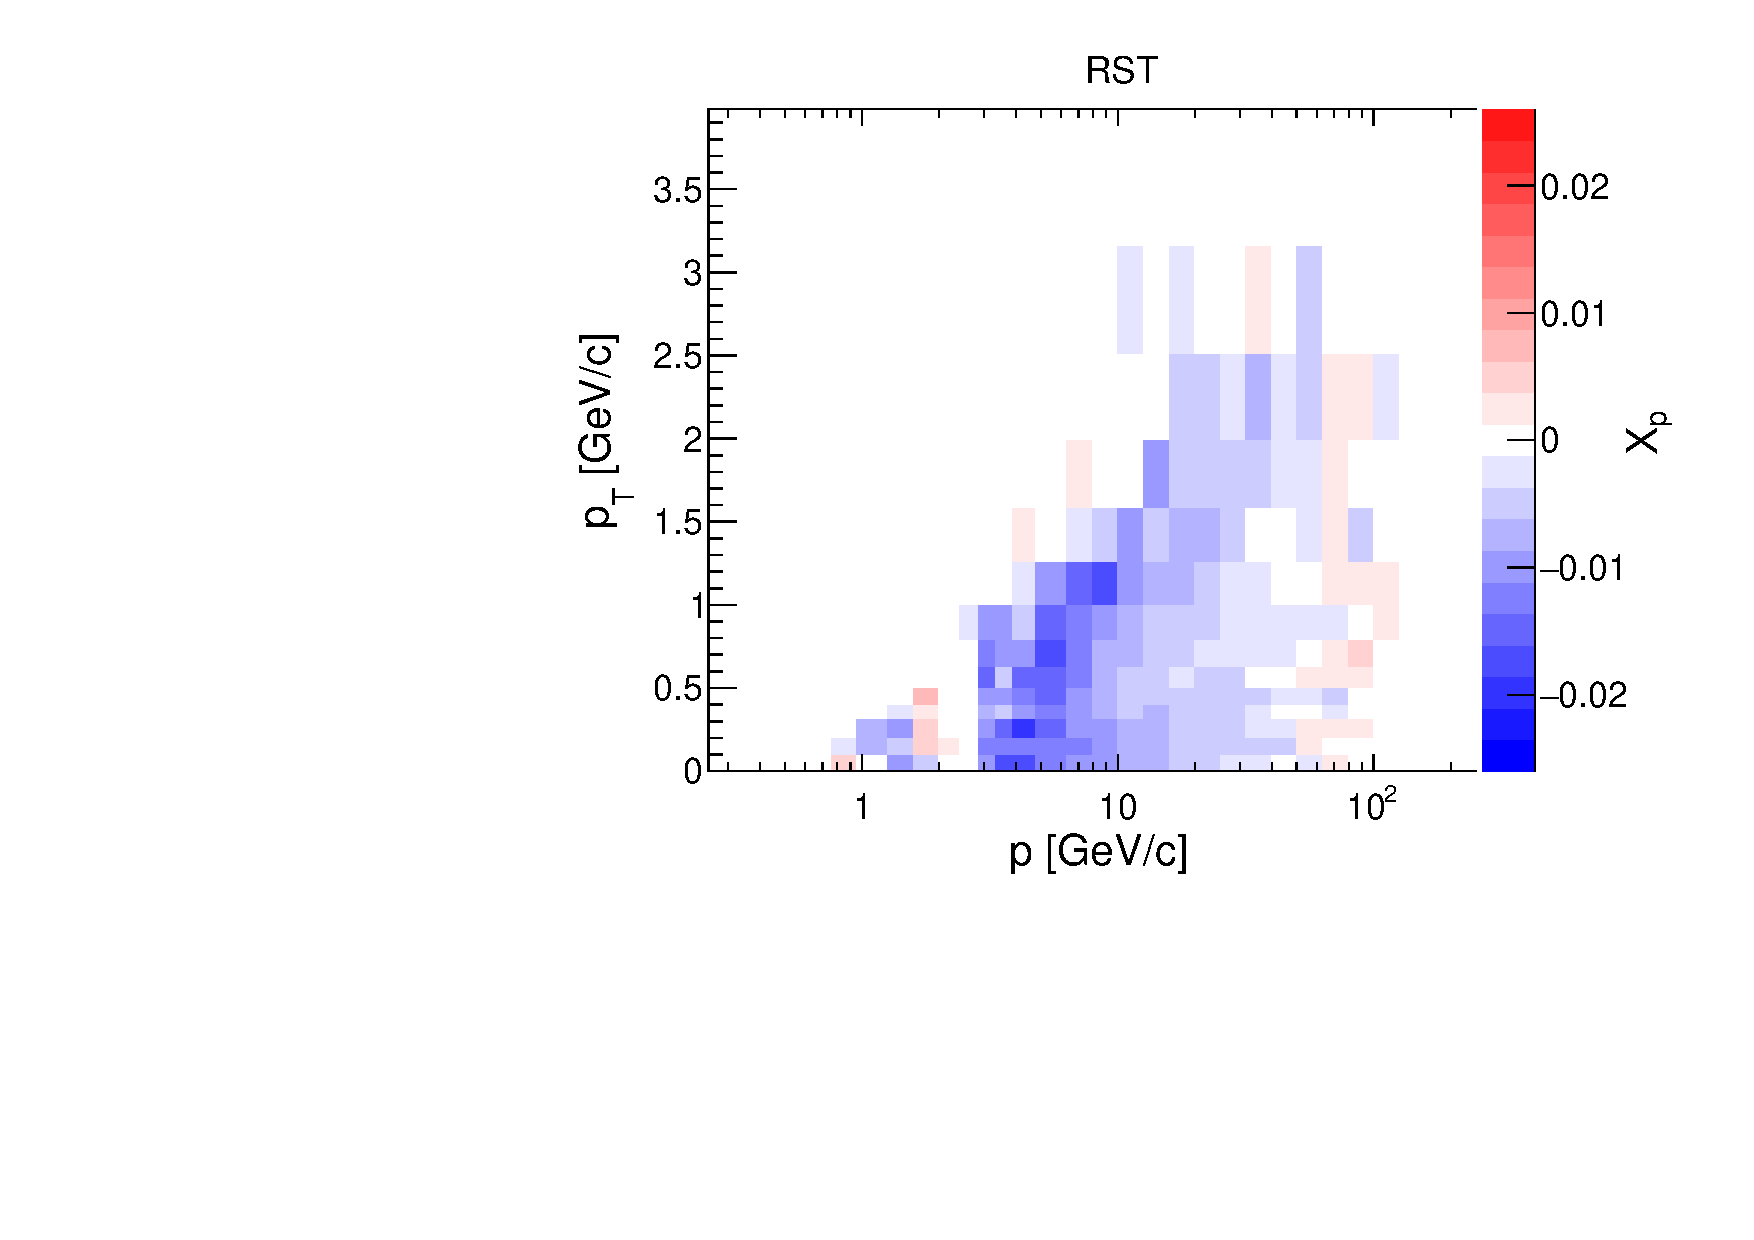
\includegraphics[clip, rviewport=0 0 1 0.94,width=0.4\textwidth]{dedx/model_350_v0_m4}
  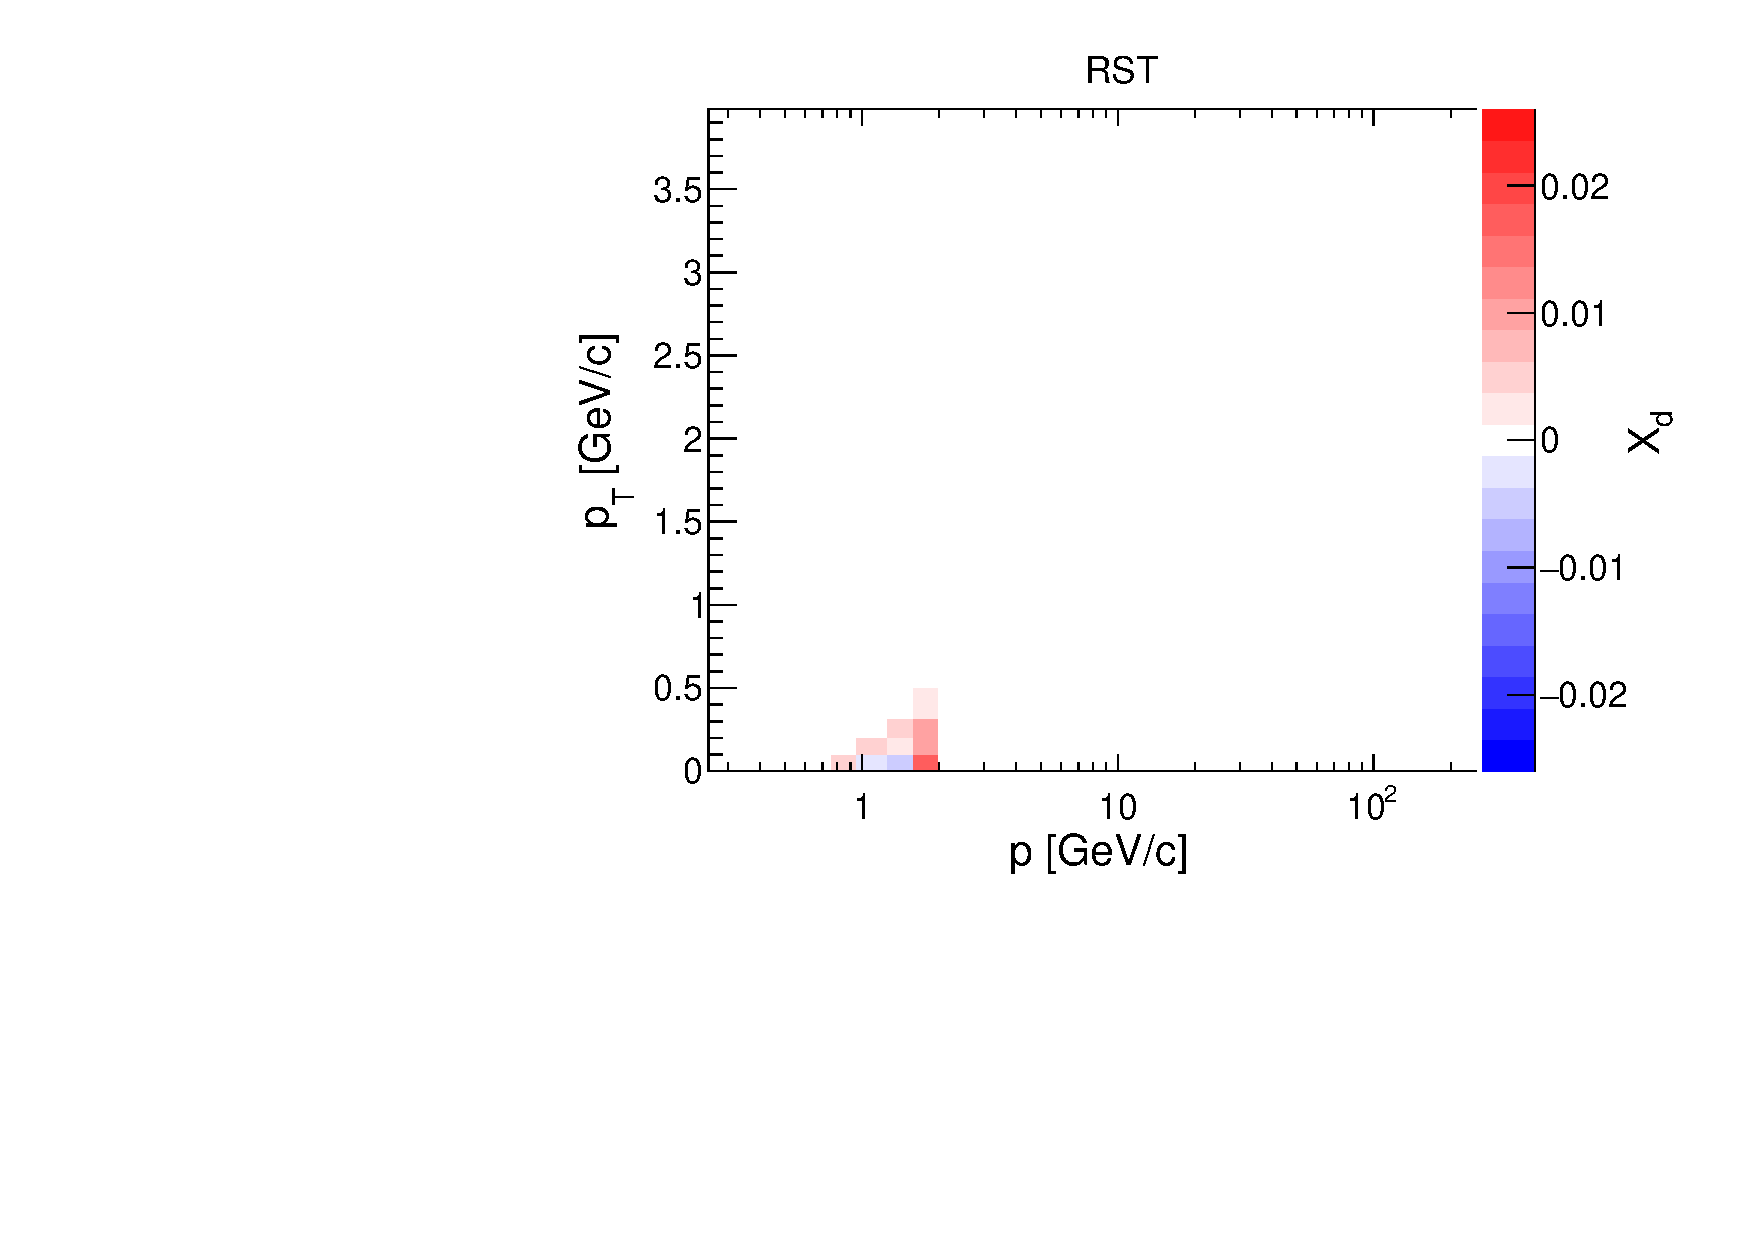
\includegraphics[clip, rviewport=0 0 1 0.94,width=0.4\textwidth]{dedx/model_350_v0_m5}
  \caption{Calibration constants obtained from the fit of the RST dataset at 350 \GeVc.}
  \label{fig:hadron:dedx:fit:cal350r}
\end{figure}

%%%%%%%%%% CAL %%%%%%%%%%%%%%
\begin{figure}
  \centering
  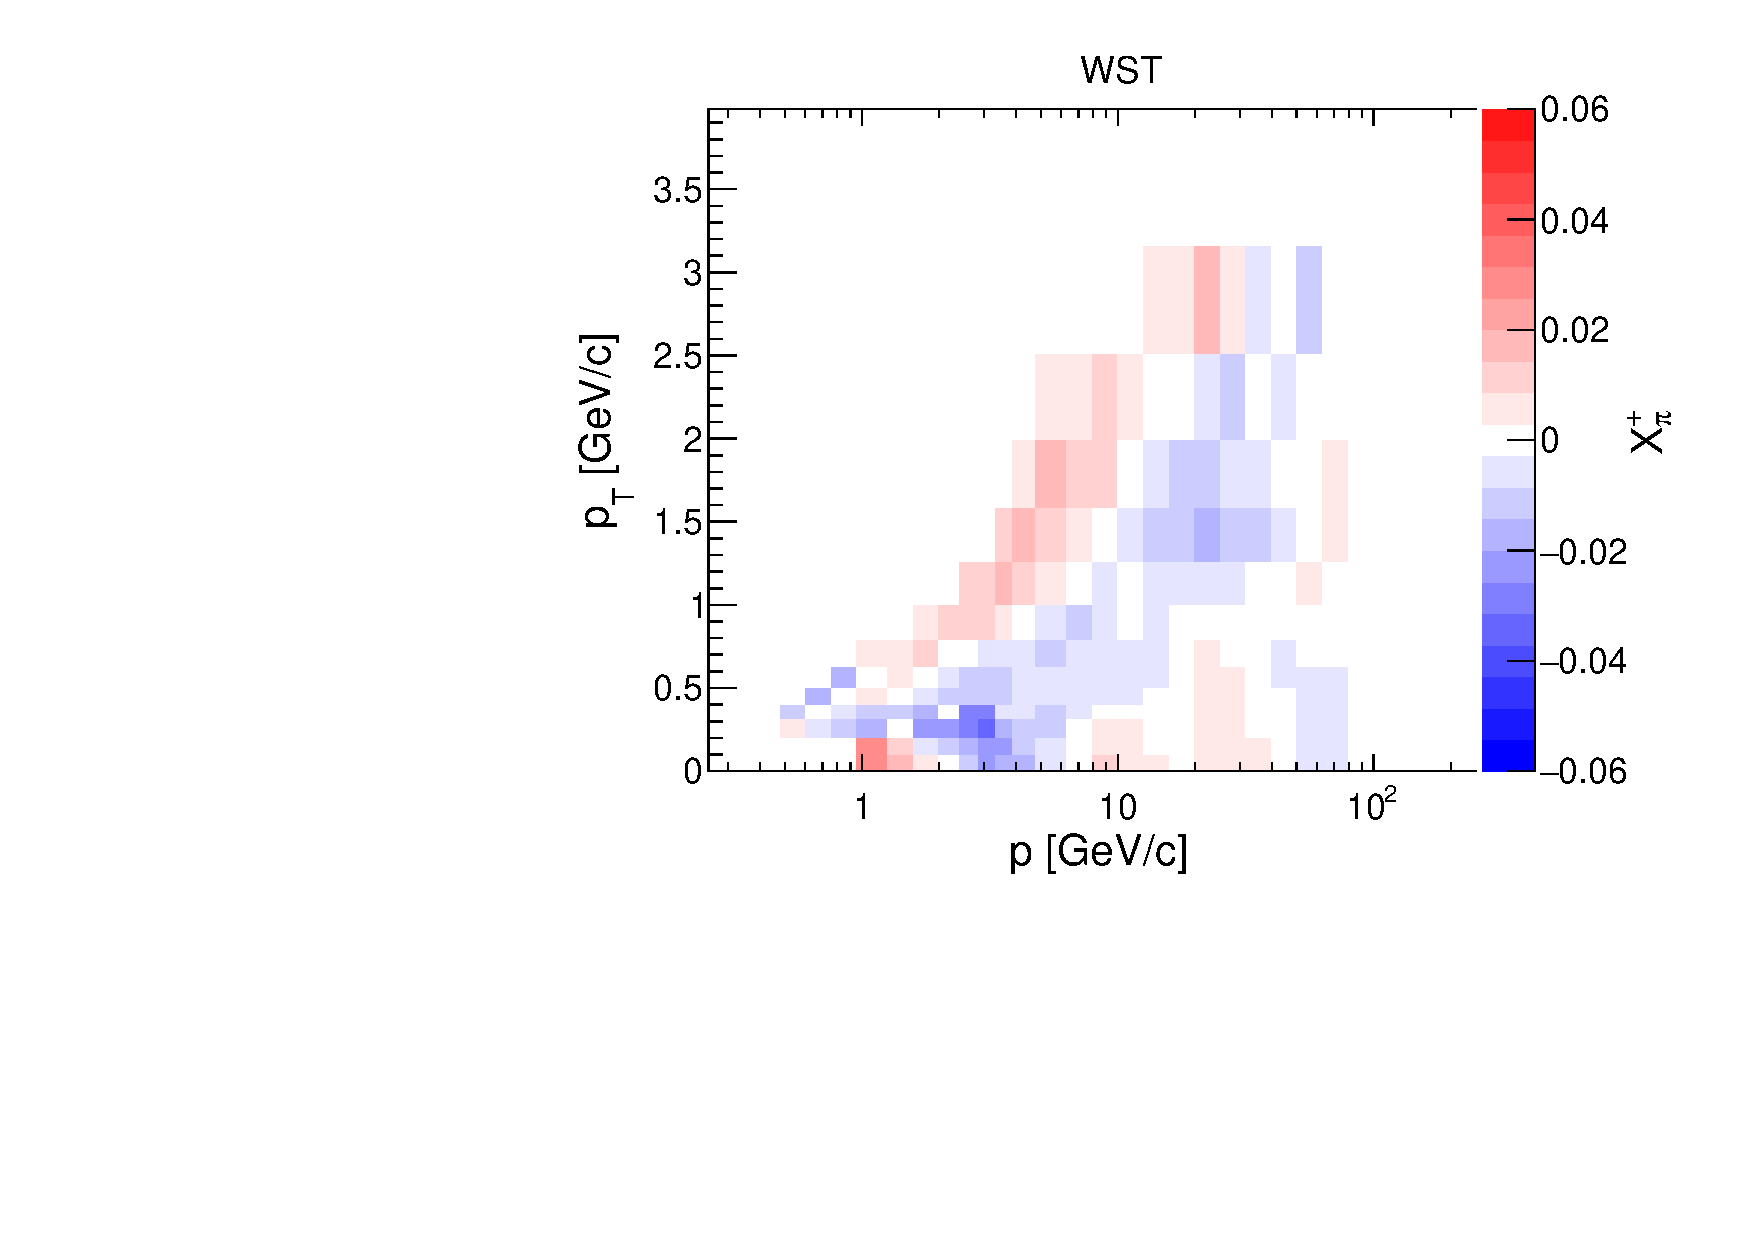
\includegraphics[clip, rviewport=0 0 1 0.94,width=0.4\textwidth]{dedx/model_350_v1_m0}
  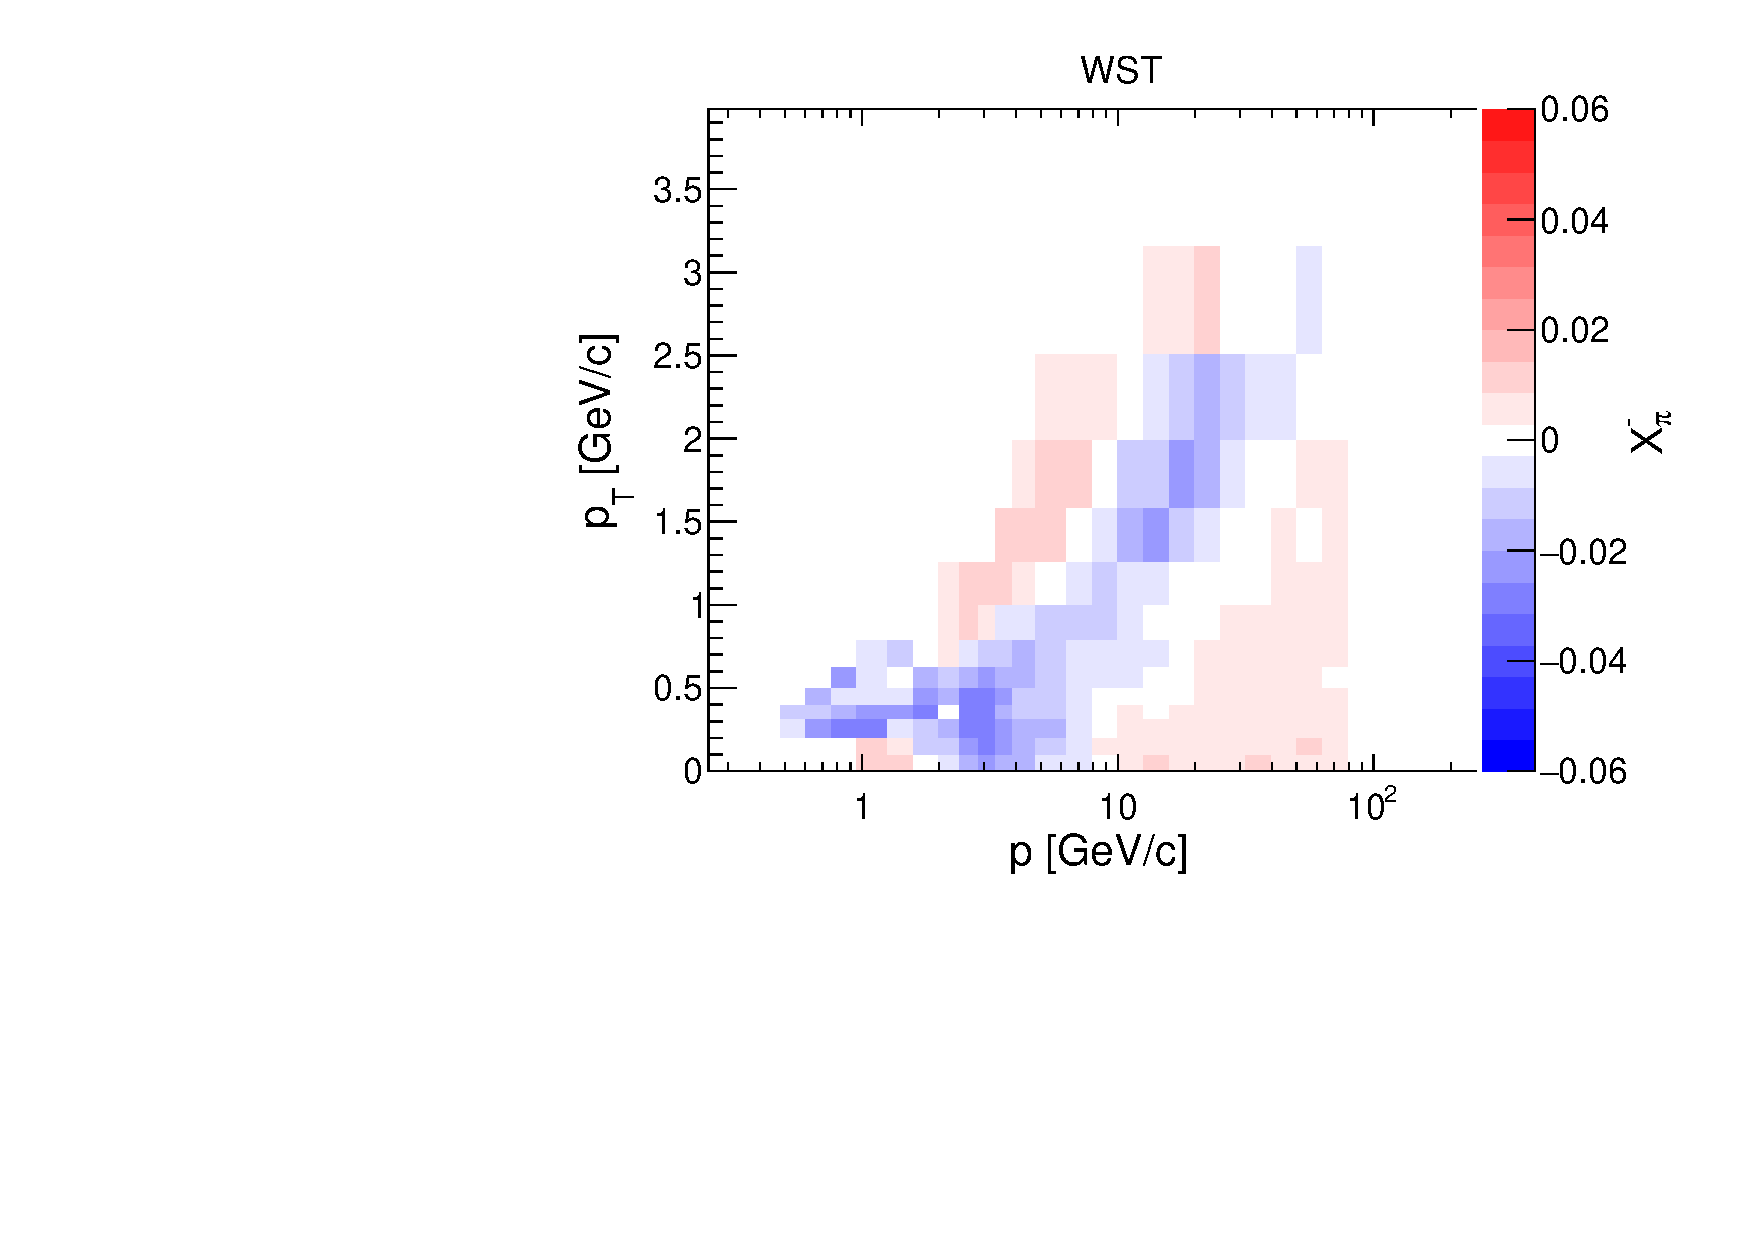
\includegraphics[clip, rviewport=0 0 1 0.94,width=0.4\textwidth]{dedx/model_350_v1_m1}

  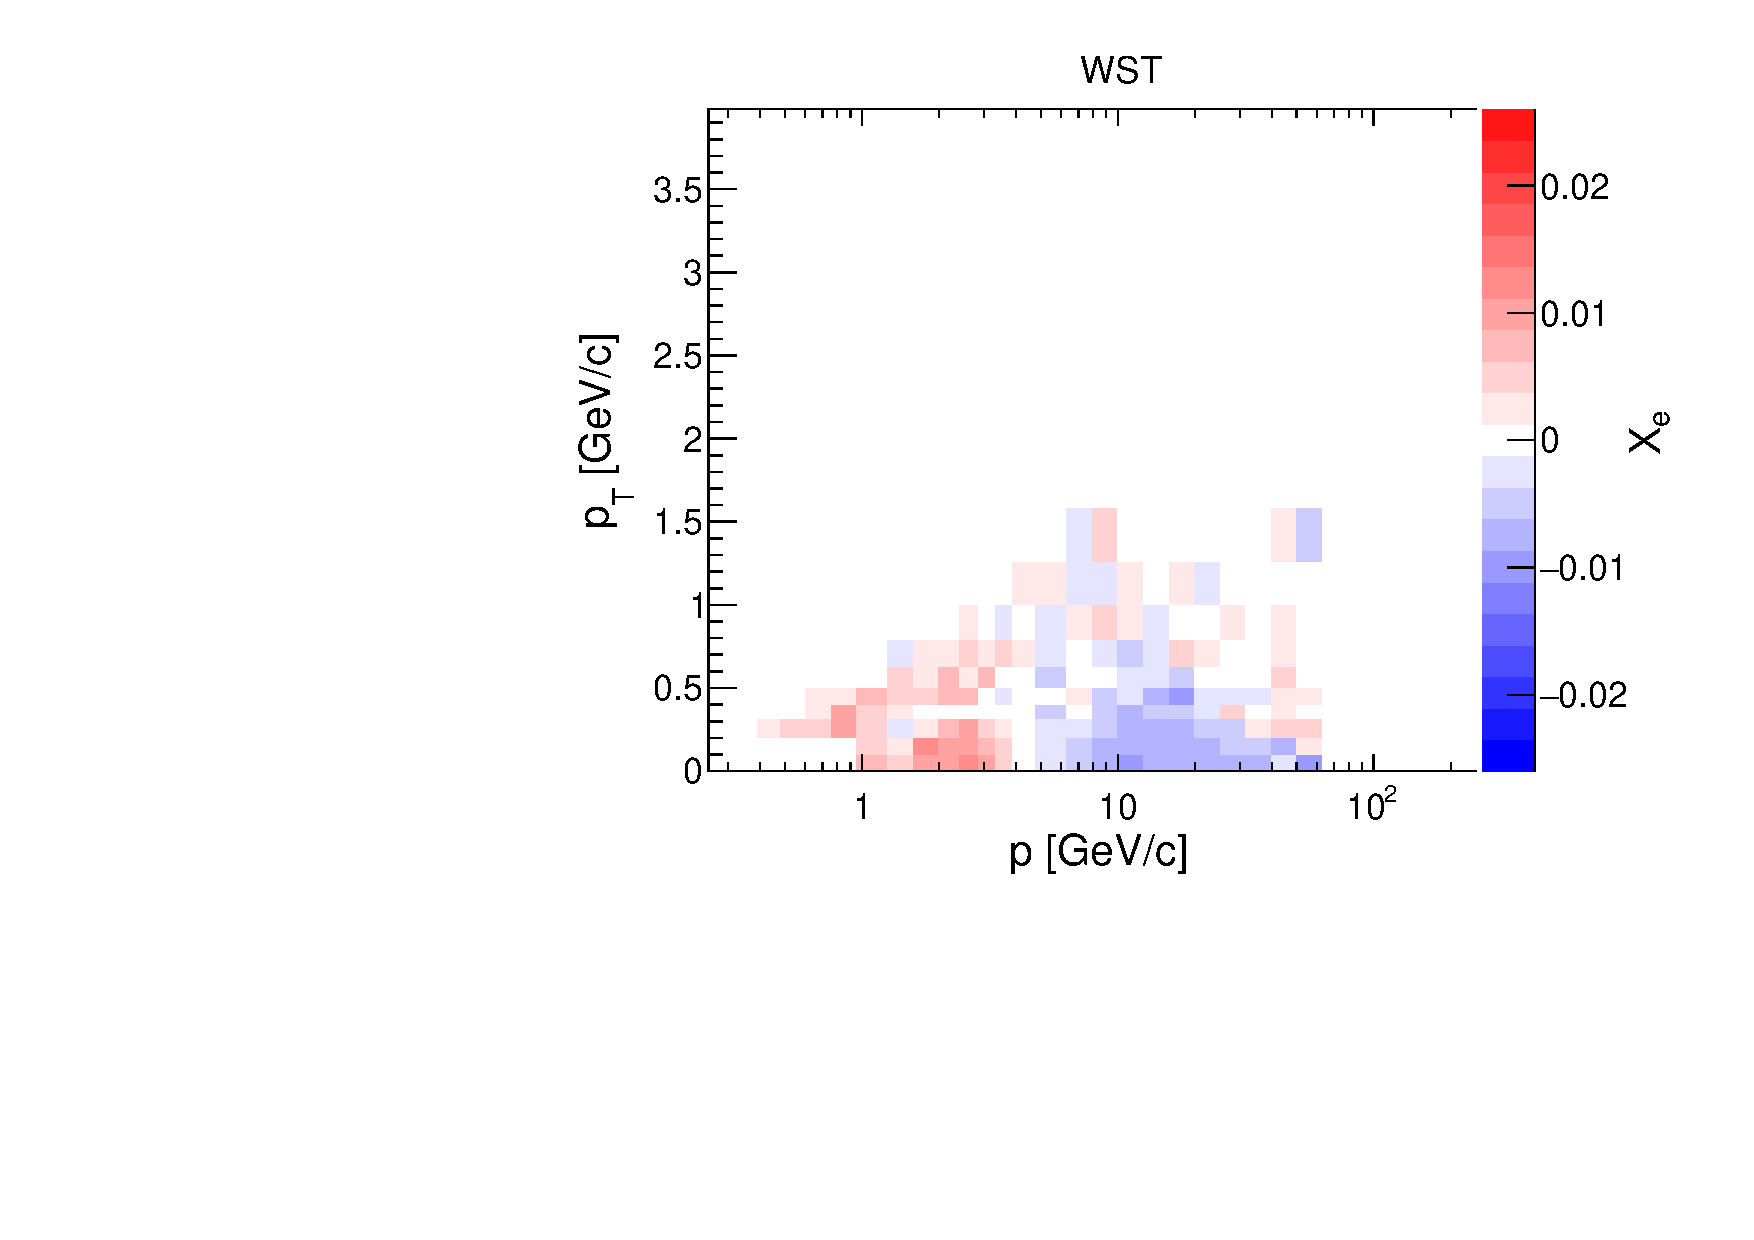
\includegraphics[clip, rviewport=0 0 1 0.94,width=0.4\textwidth]{dedx/model_350_v1_m2}
  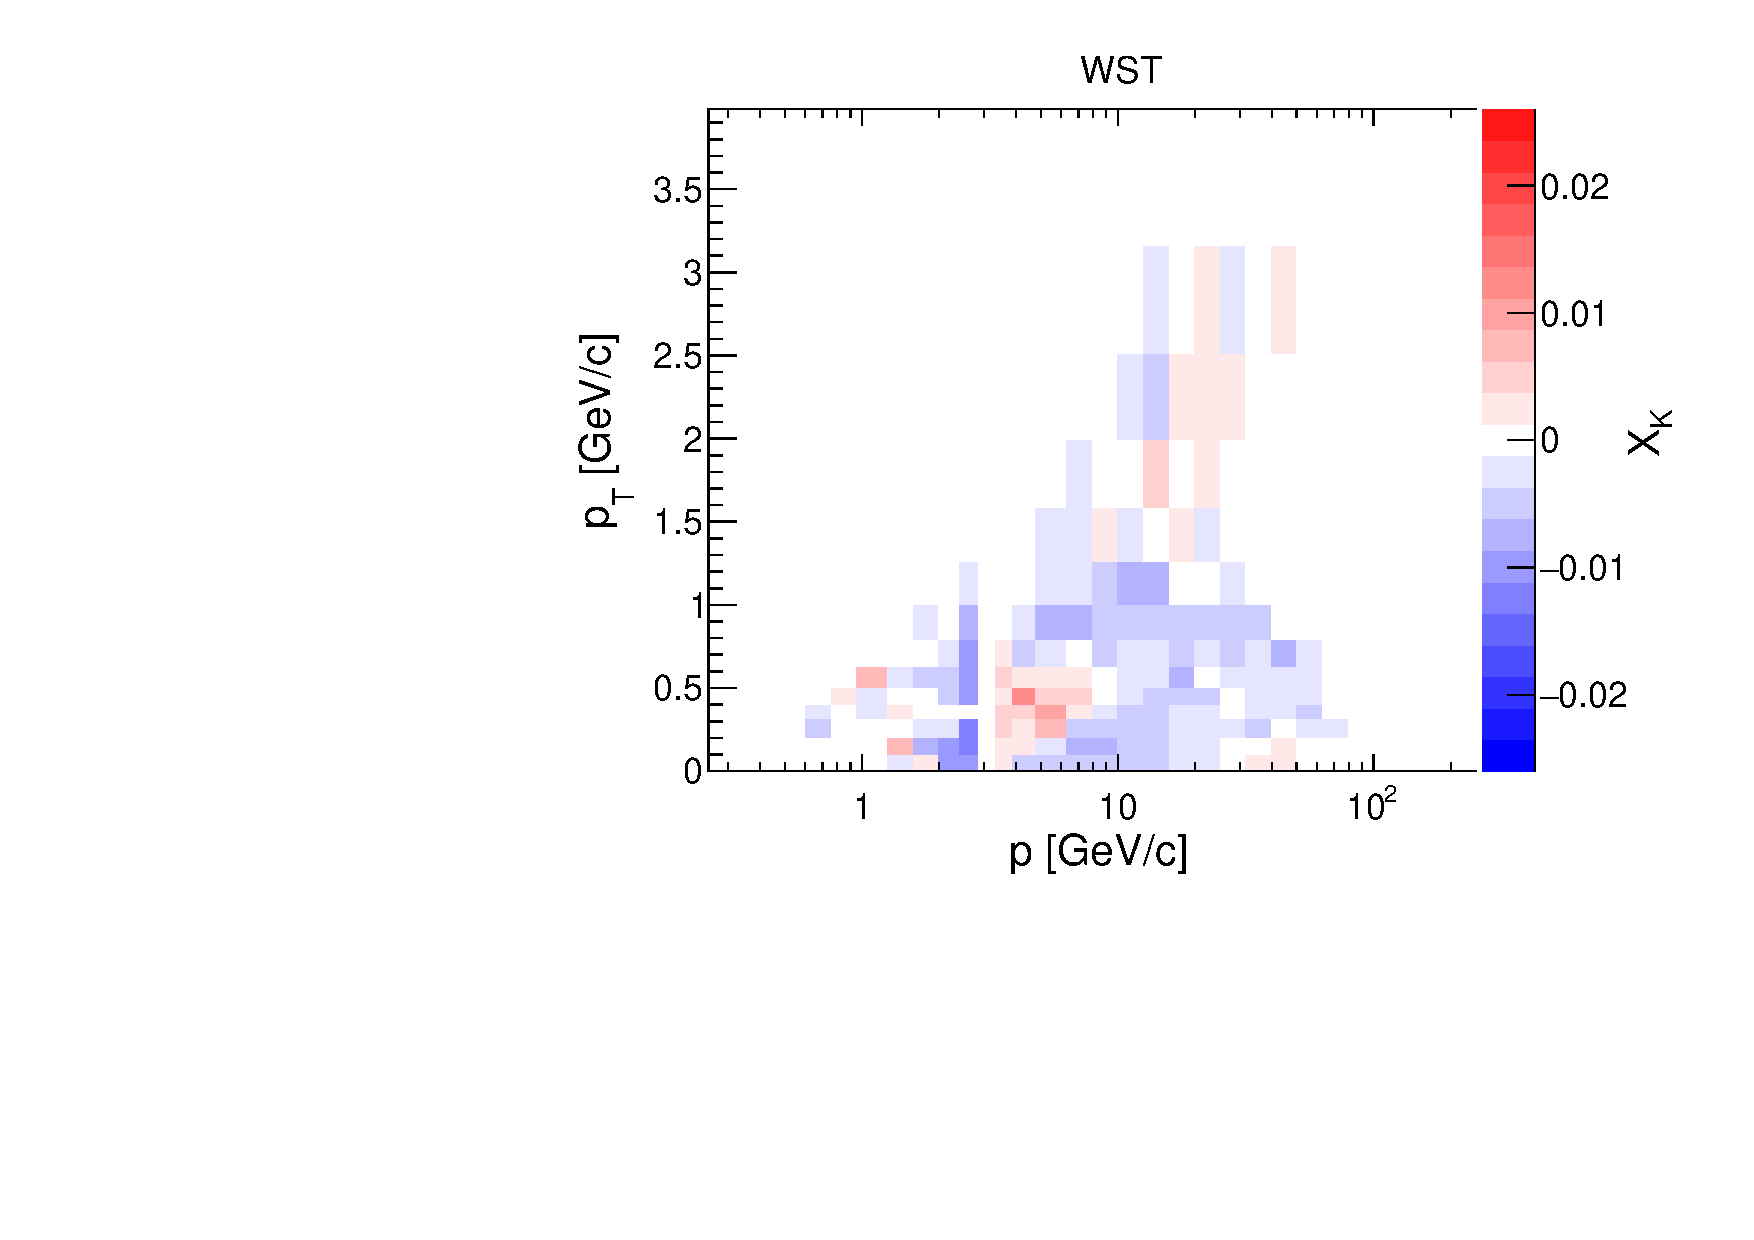
\includegraphics[clip, rviewport=0 0 1 0.94,width=0.4\textwidth]{dedx/model_350_v1_m3}

  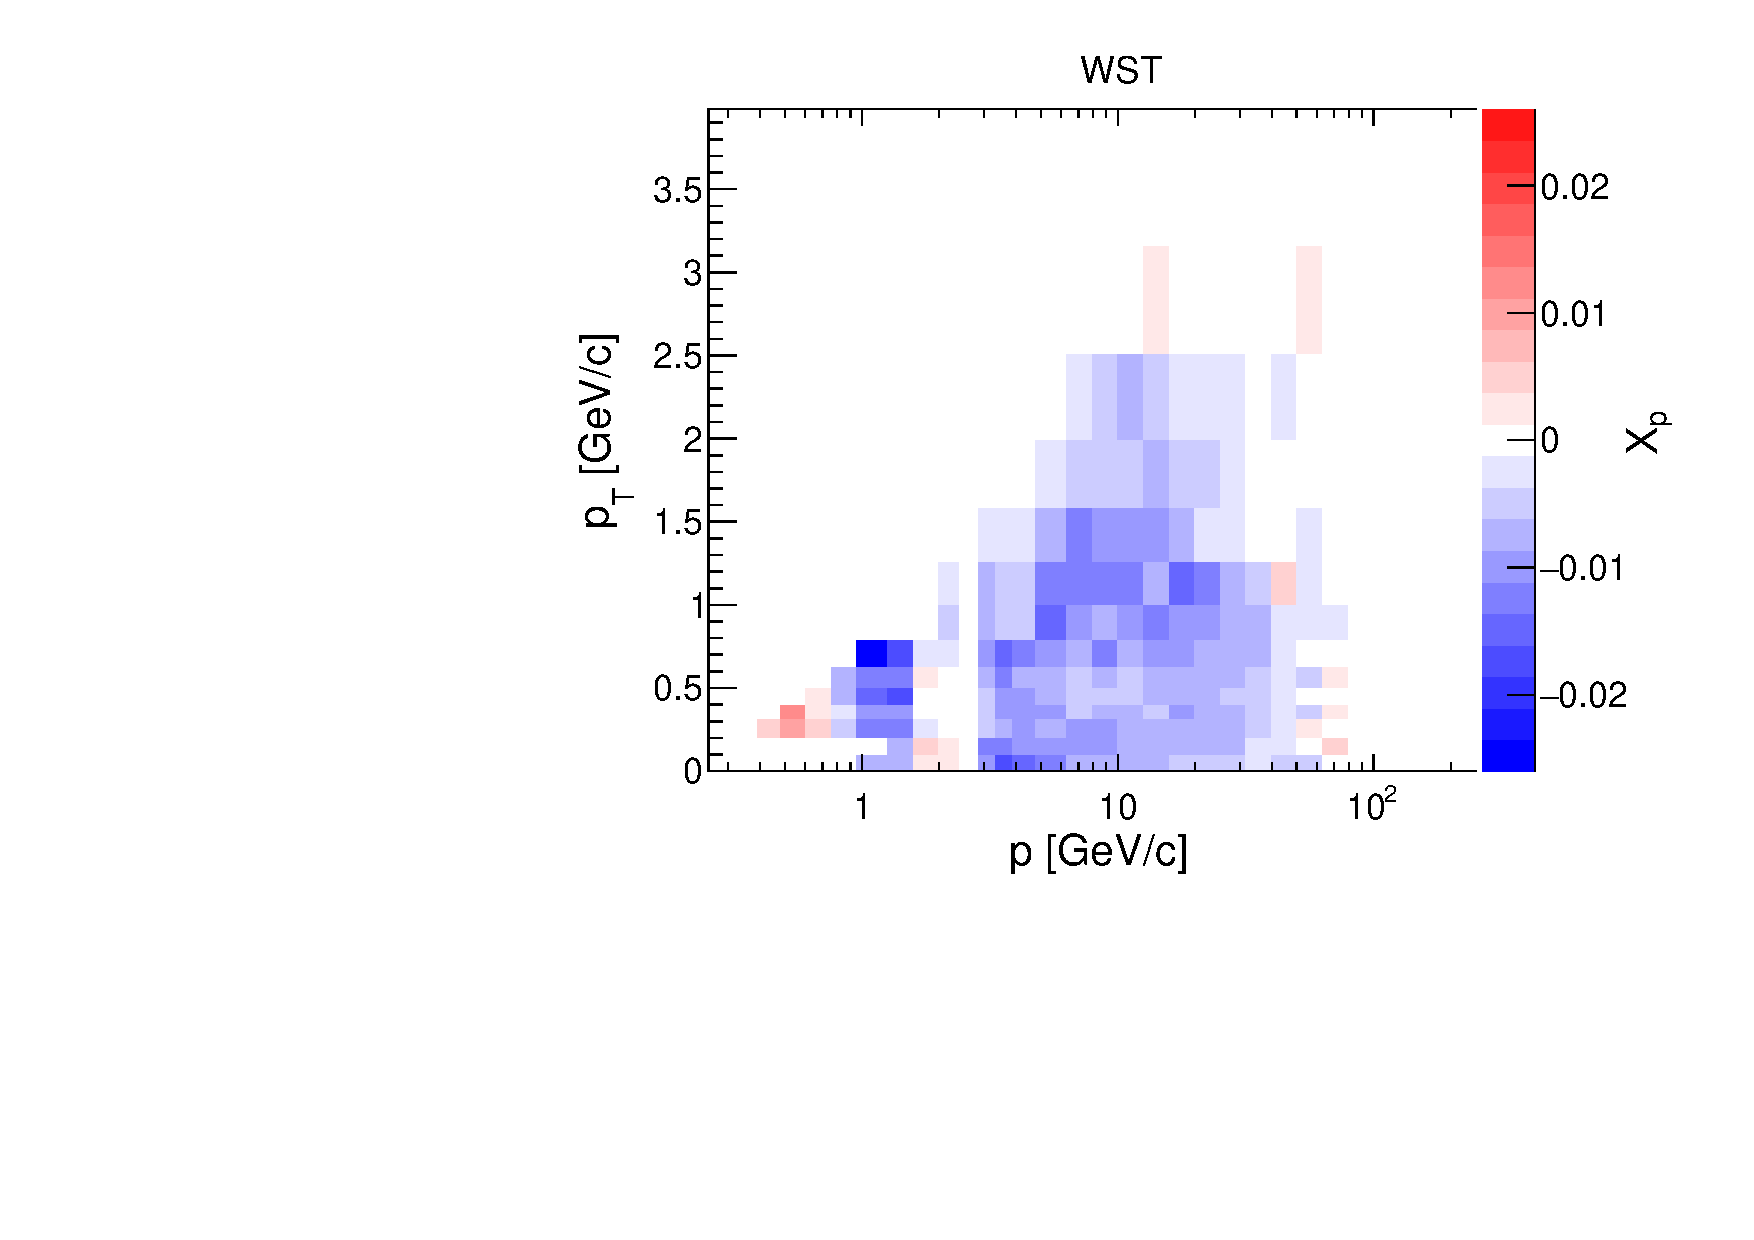
\includegraphics[clip, rviewport=0 0 1 0.94,width=0.4\textwidth]{dedx/model_350_v1_m4}
  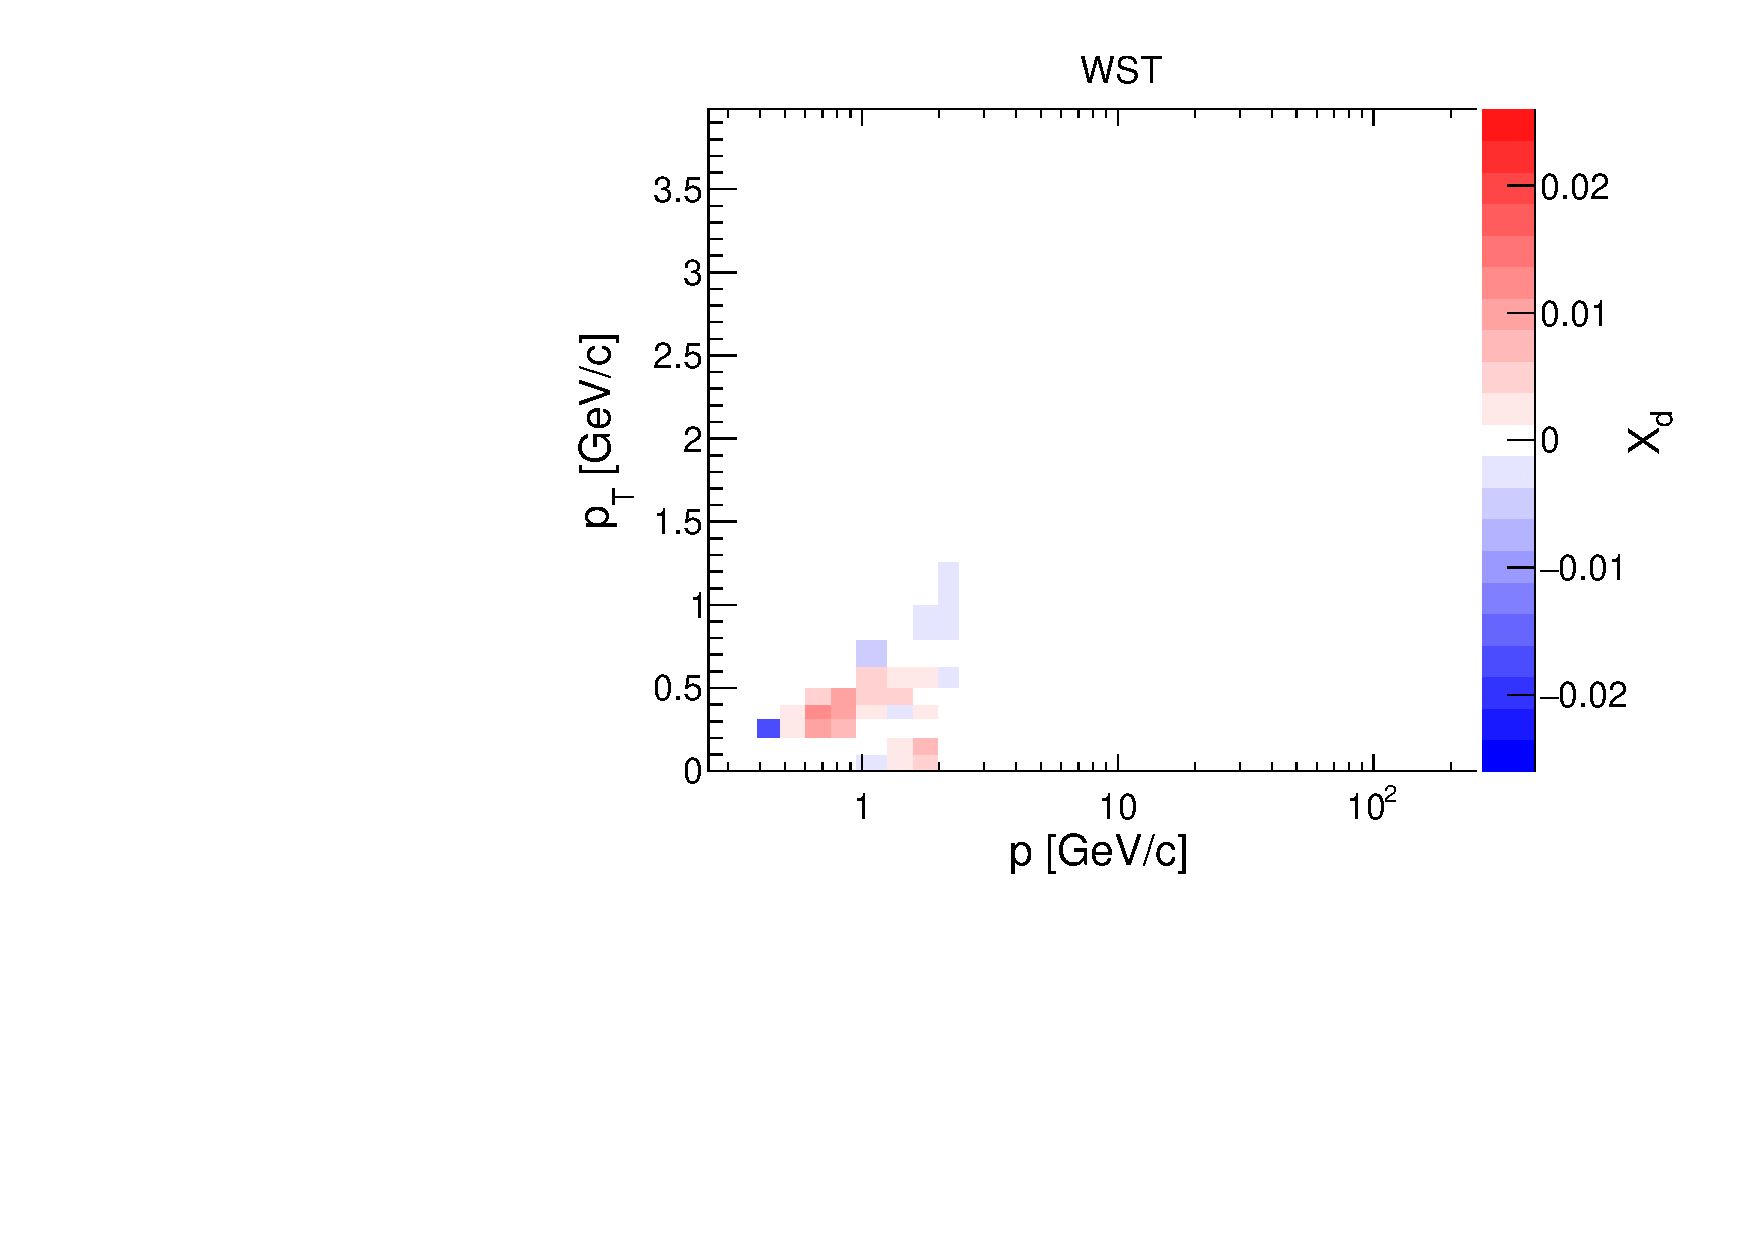
\includegraphics[clip, rviewport=0 0 1 0.94,width=0.4\textwidth]{dedx/model_350_v1_m5}
  \caption{Calibration constants obtained from the fit of the WST dataset at 350 \GeVc.}
  \label{fig:hadron:dedx:fit:cal350w}
\end{figure}

\clearpage

%%%%%%%%%% SHAPE %%%%%%%%%%%%%%
\begin{figure}
  \centering
  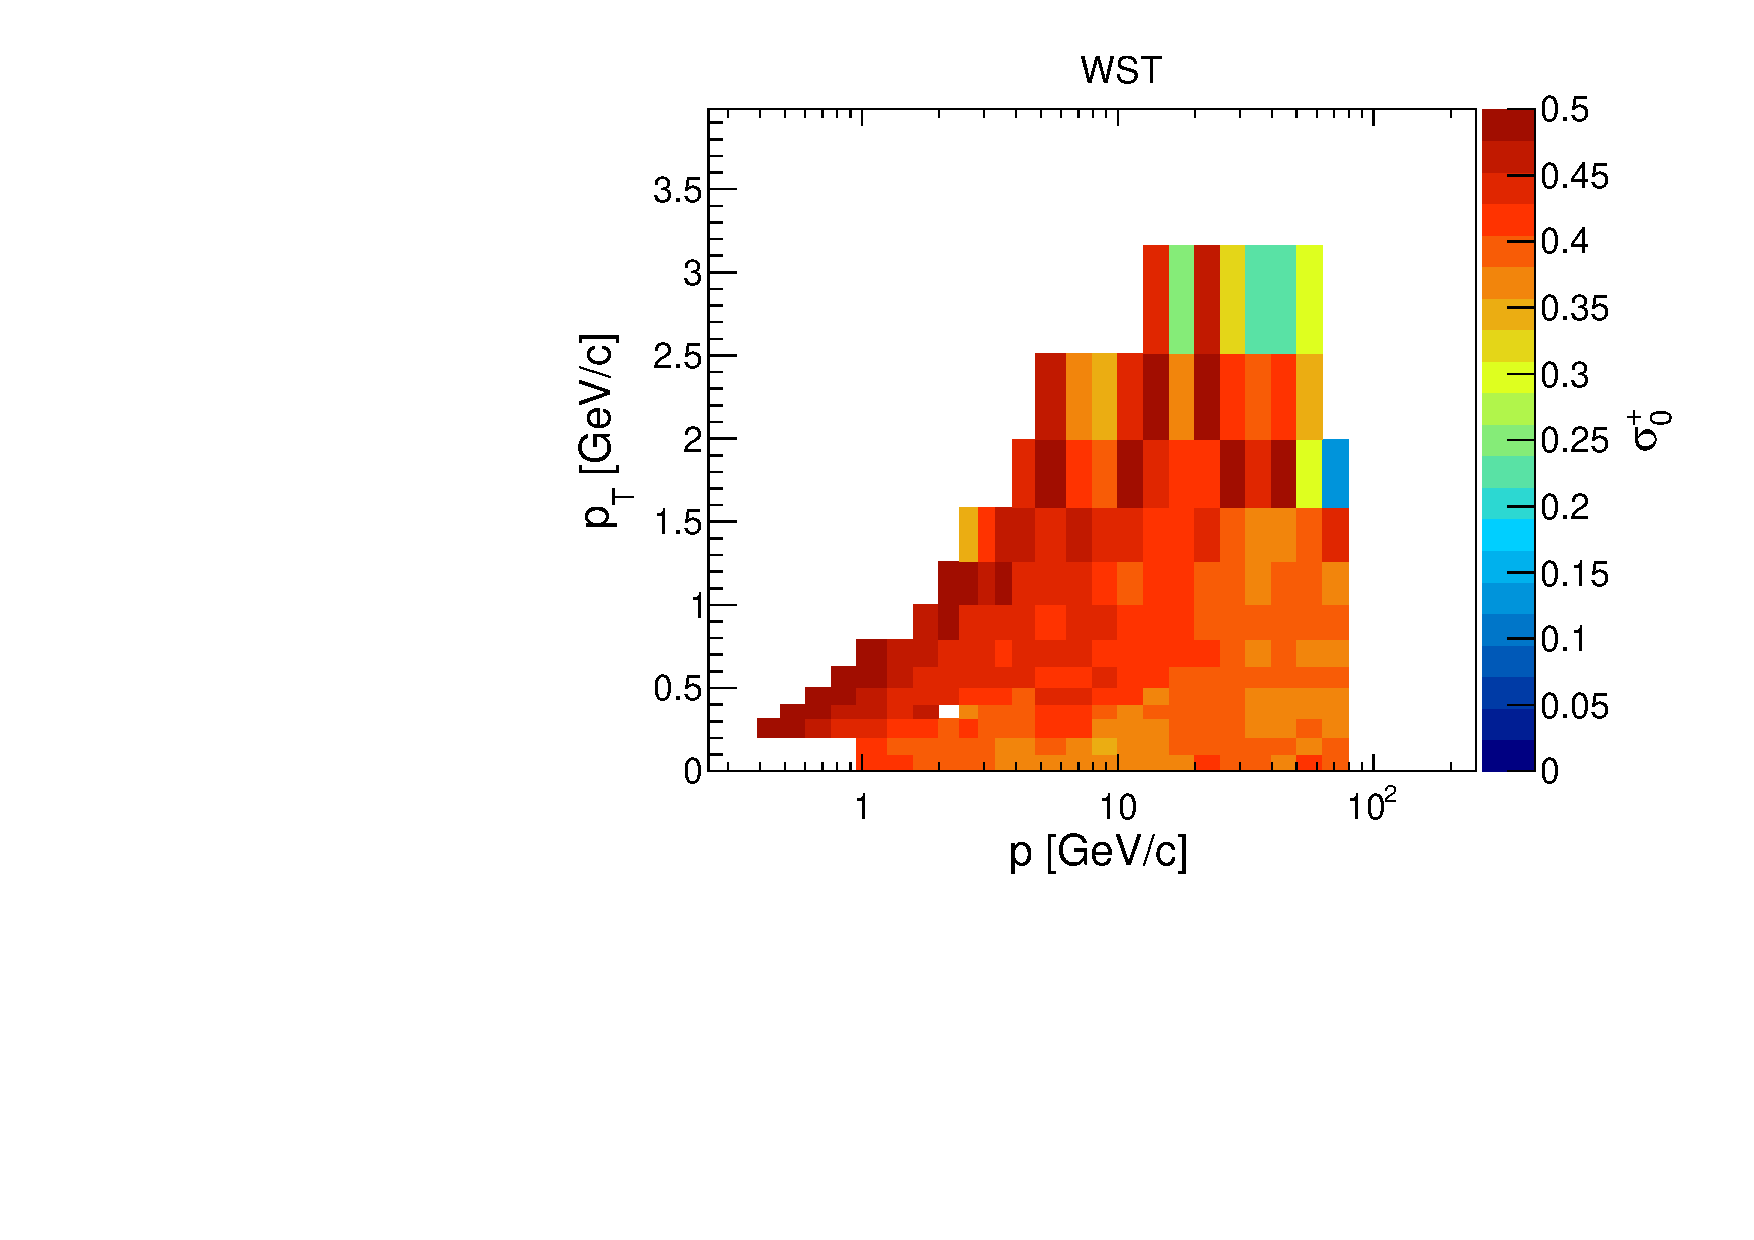
\includegraphics[clip, rviewport=0 0 1 0.94,width=0.4\textwidth]{dedx/model_158_v1_m6}
  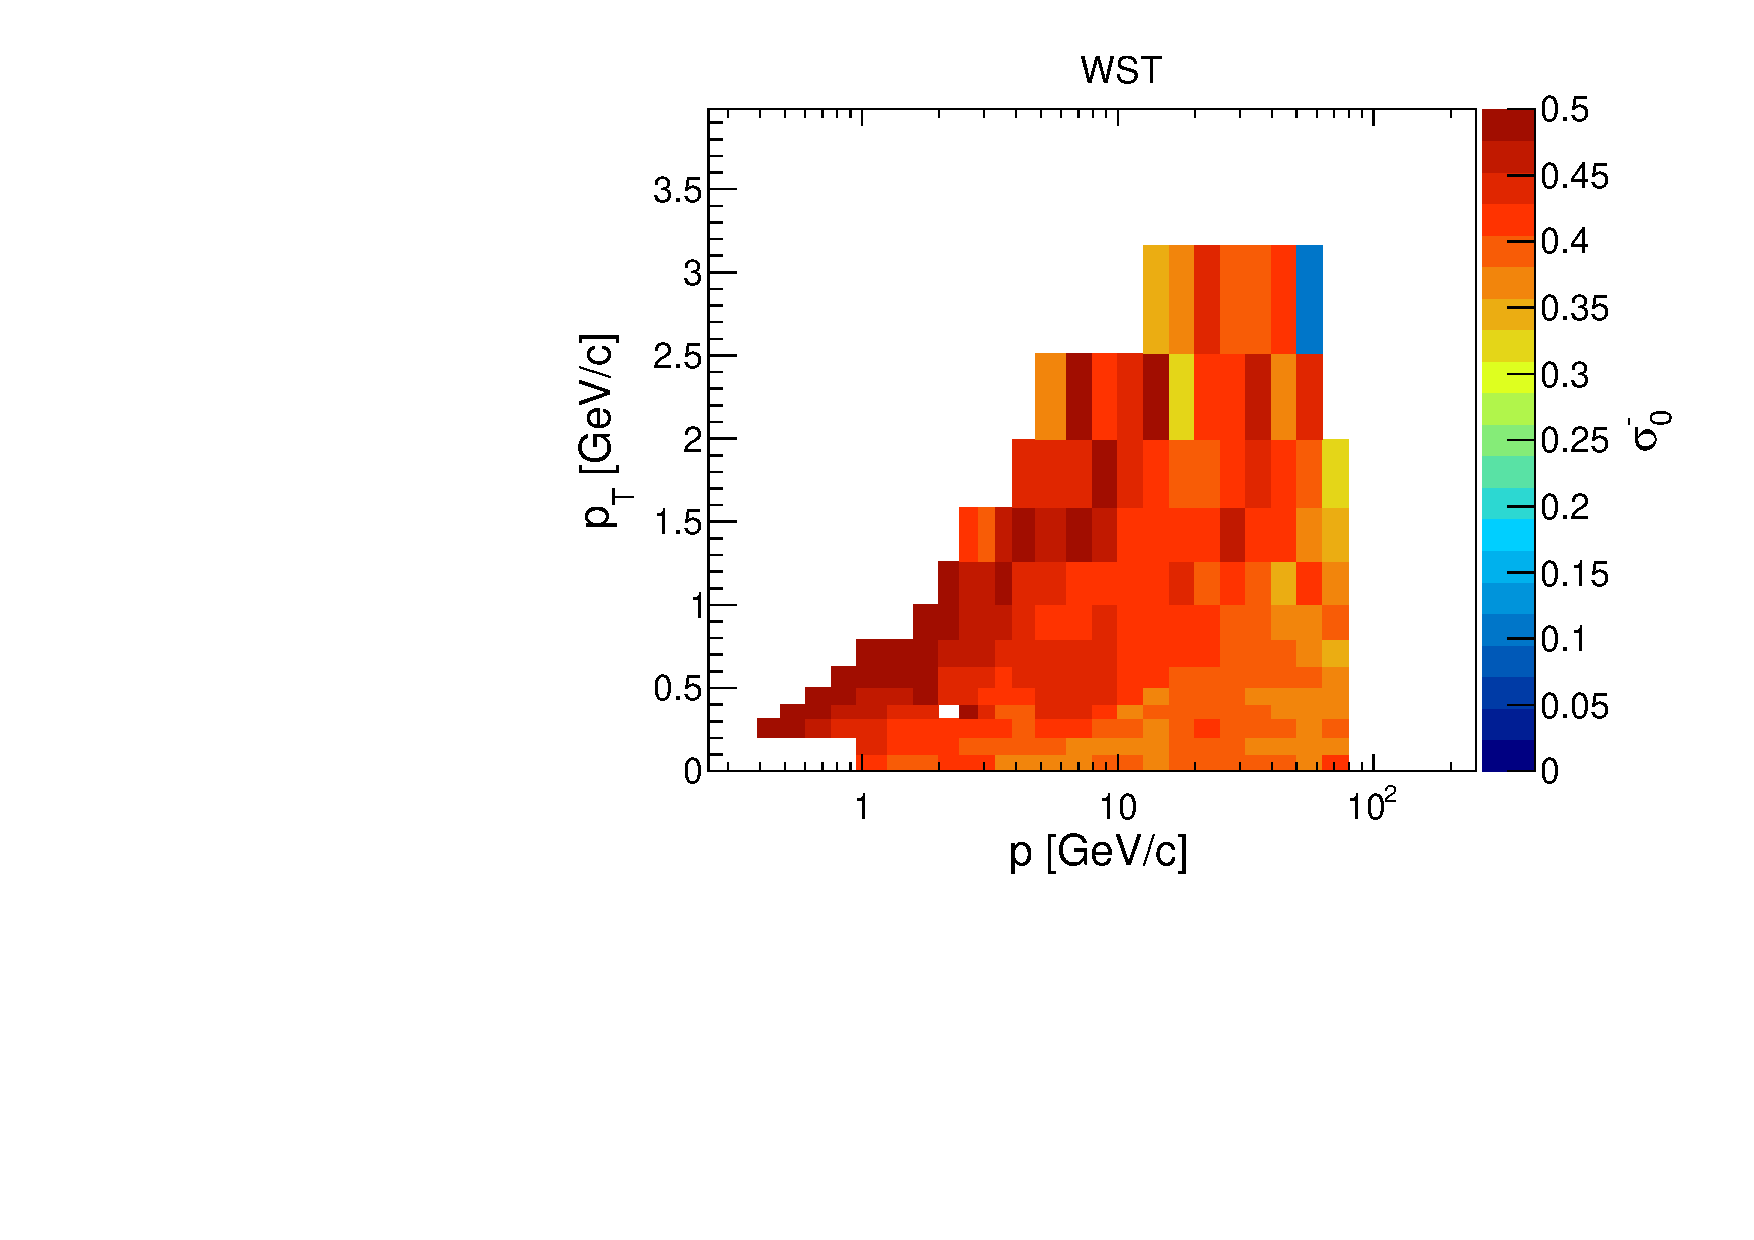
\includegraphics[clip, rviewport=0 0 1 0.94,width=0.4\textwidth]{dedx/model_158_v1_m7}

  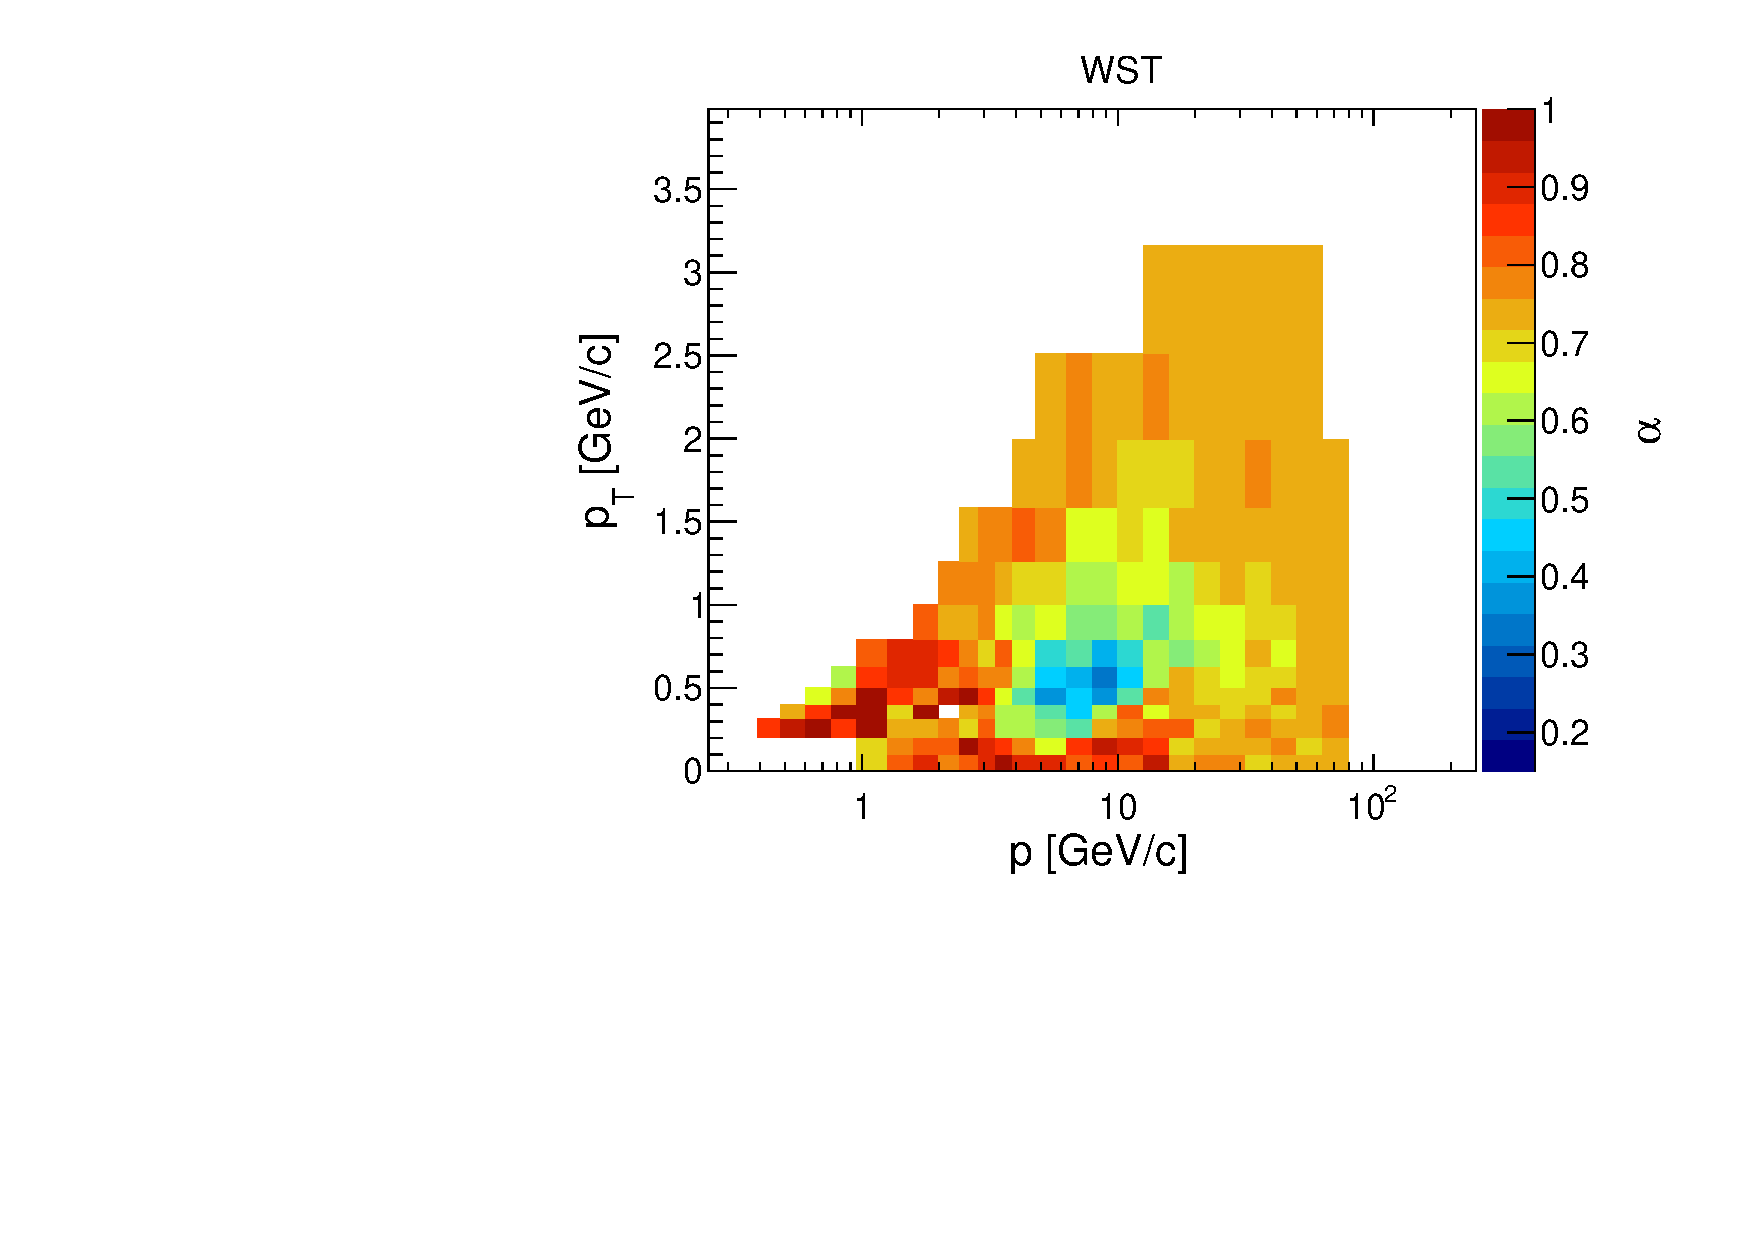
\includegraphics[clip, rviewport=0 0 1 0.94,width=0.4\textwidth]{dedx/model_158_v1_m9}
  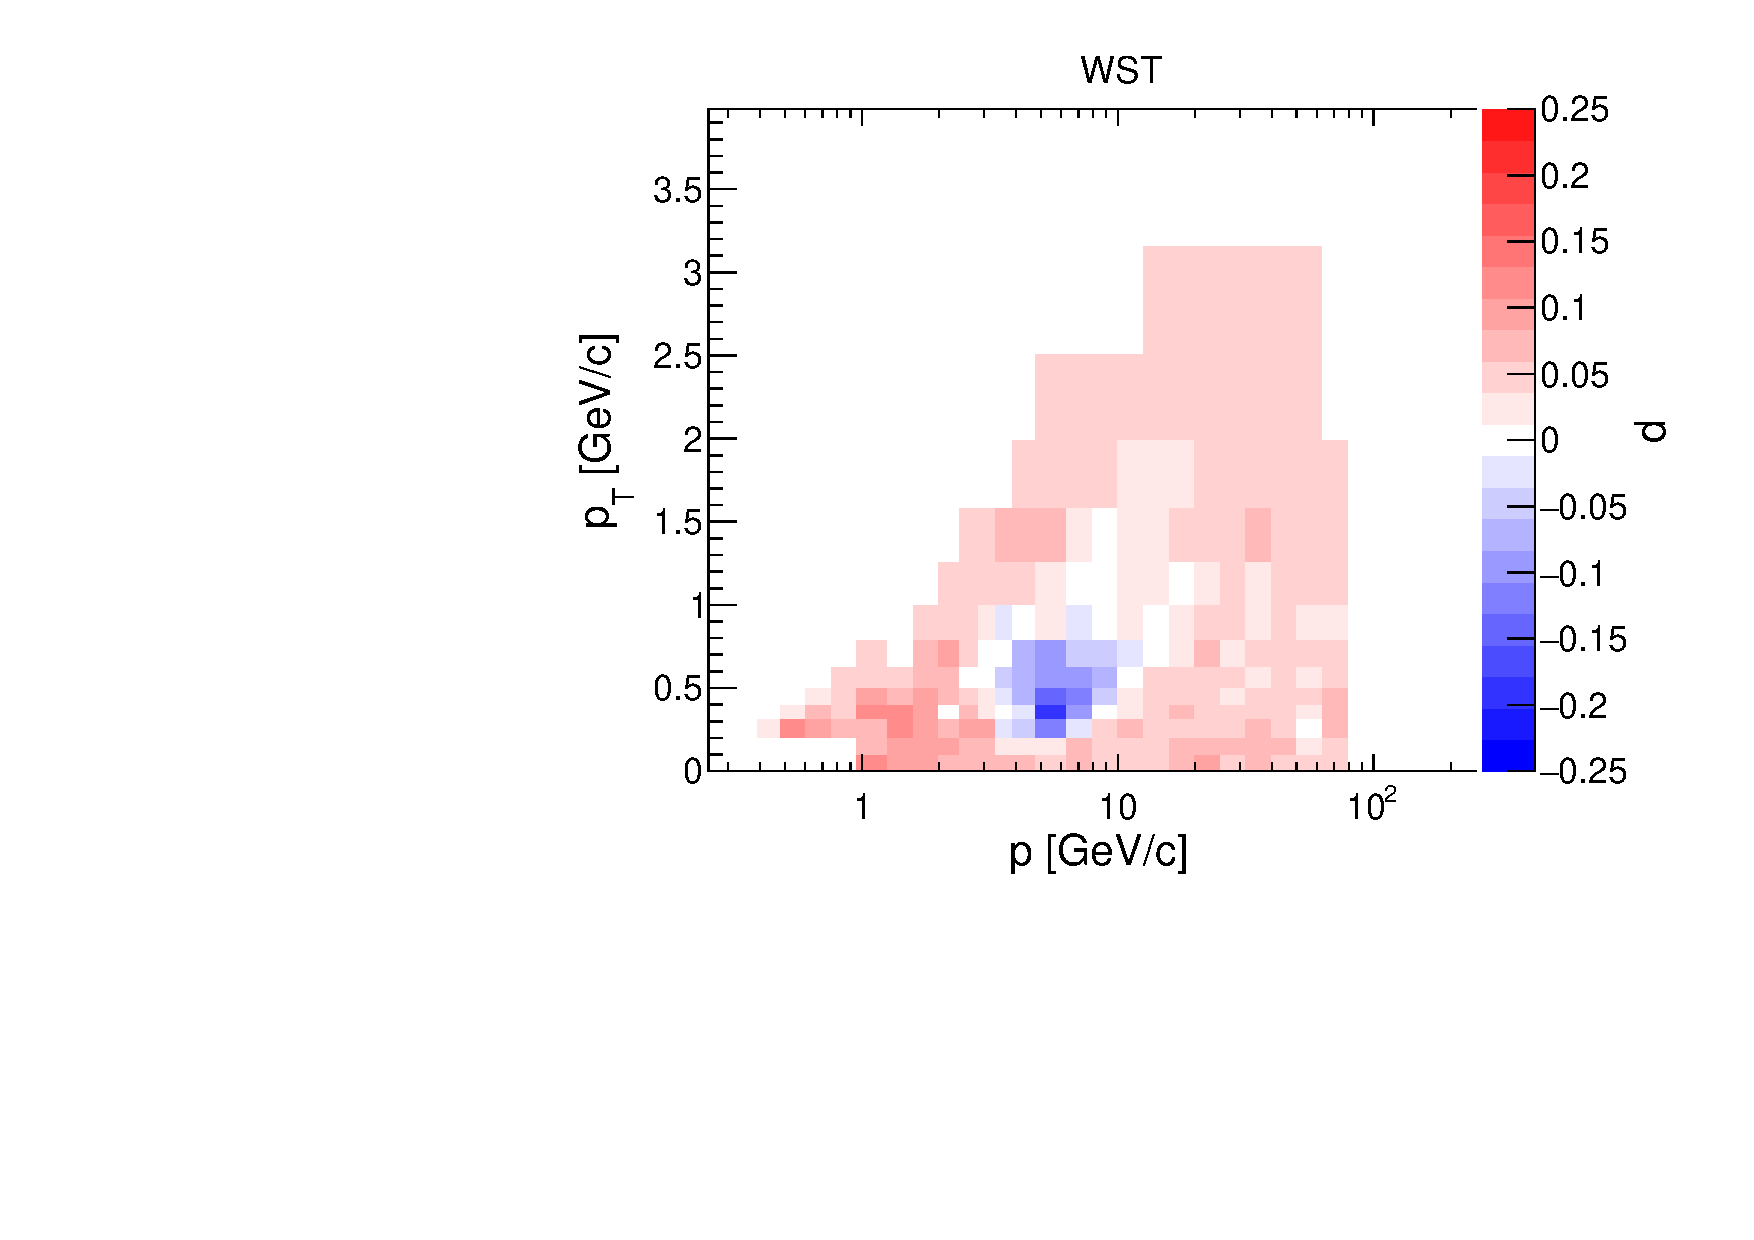
\includegraphics[clip, rviewport=0 0 1 0.94,width=0.4\textwidth]{dedx/model_158_v1_m10}
  \caption{Shape parameters obtained from the fit of the WST dataset at 158 \GeVc.}
  \label{fig:hadron:dedx:fit:shape158w}
\end{figure}

%%%%%%%%%% SHAPE %%%%%%%%%%%%%%
\begin{figure}
  \centering
  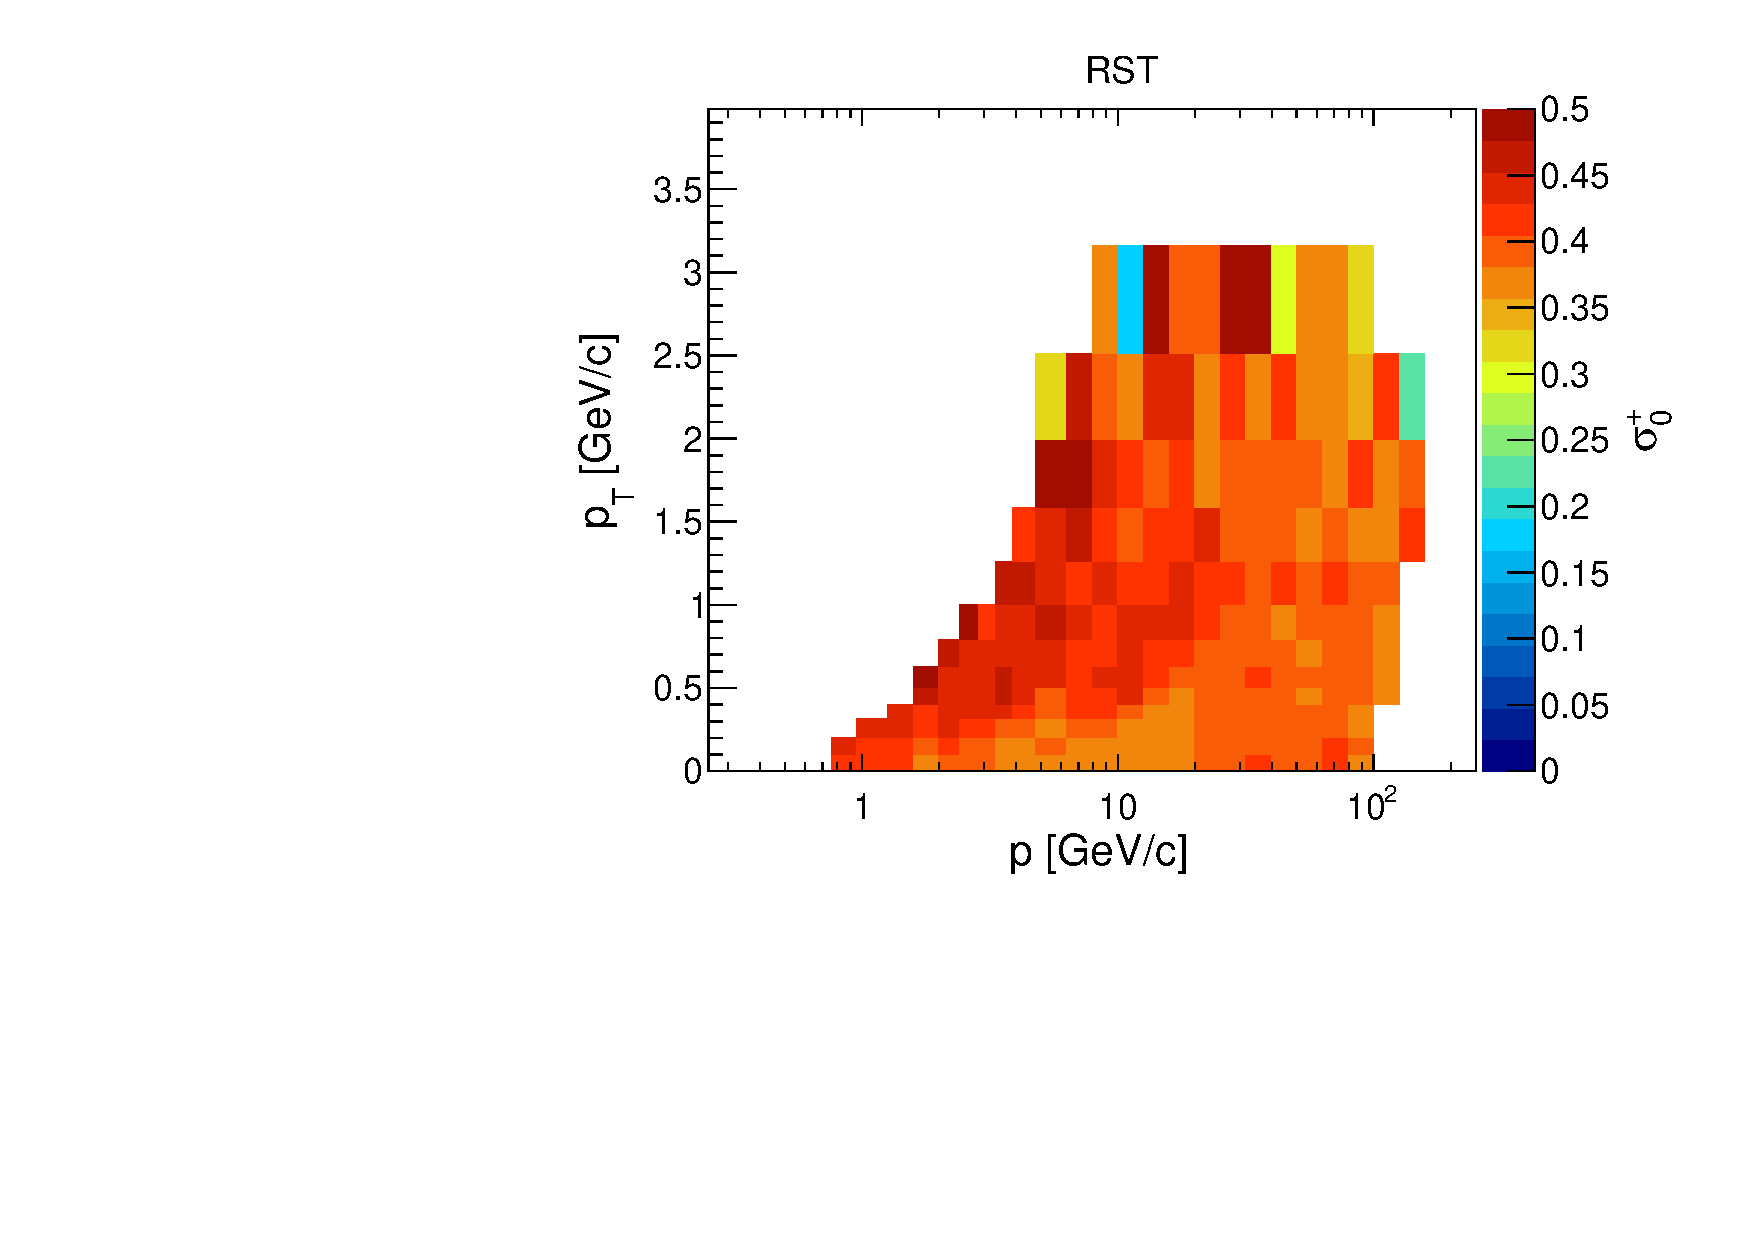
\includegraphics[clip, rviewport=0 0 1 0.94,width=0.4\textwidth]{dedx/model_350_v0_m6}
  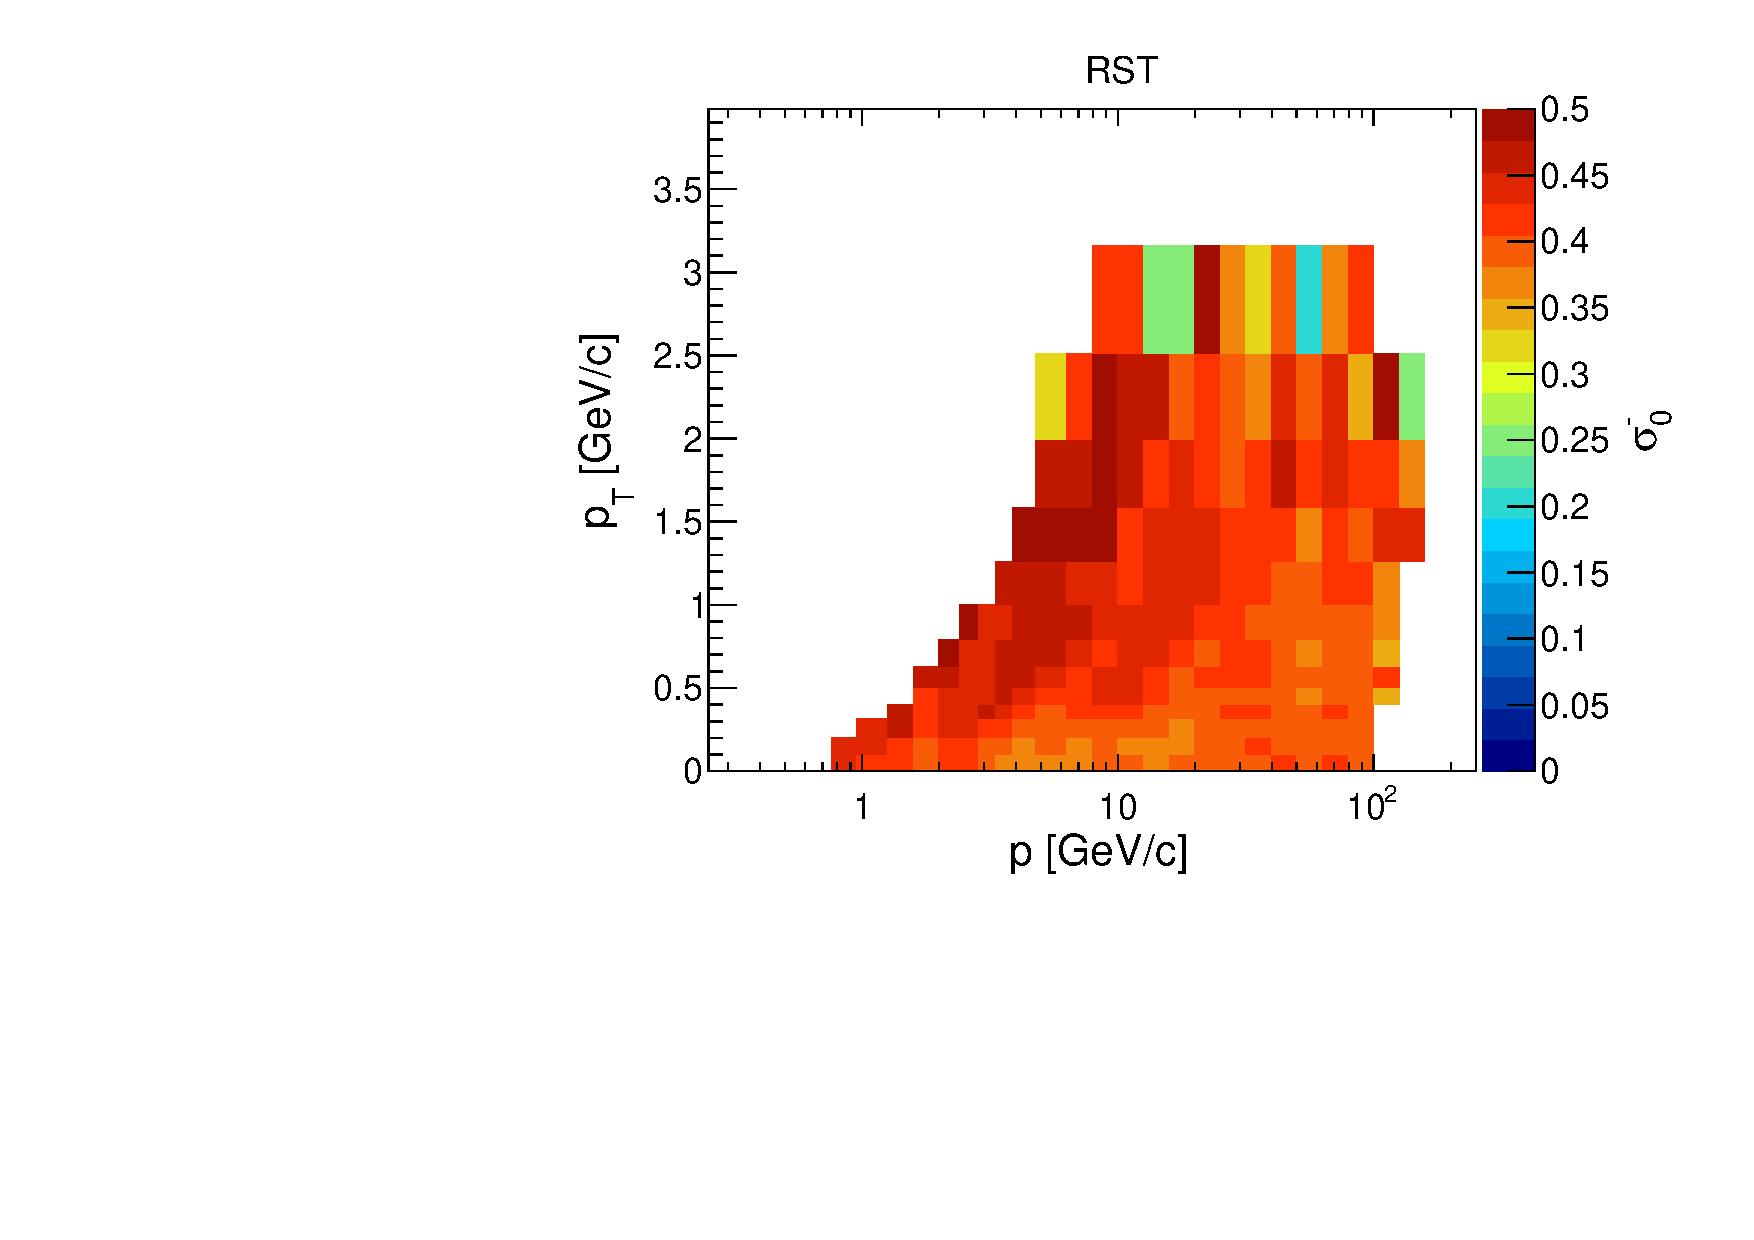
\includegraphics[clip, rviewport=0 0 1 0.94,width=0.4\textwidth]{dedx/model_350_v0_m7}

  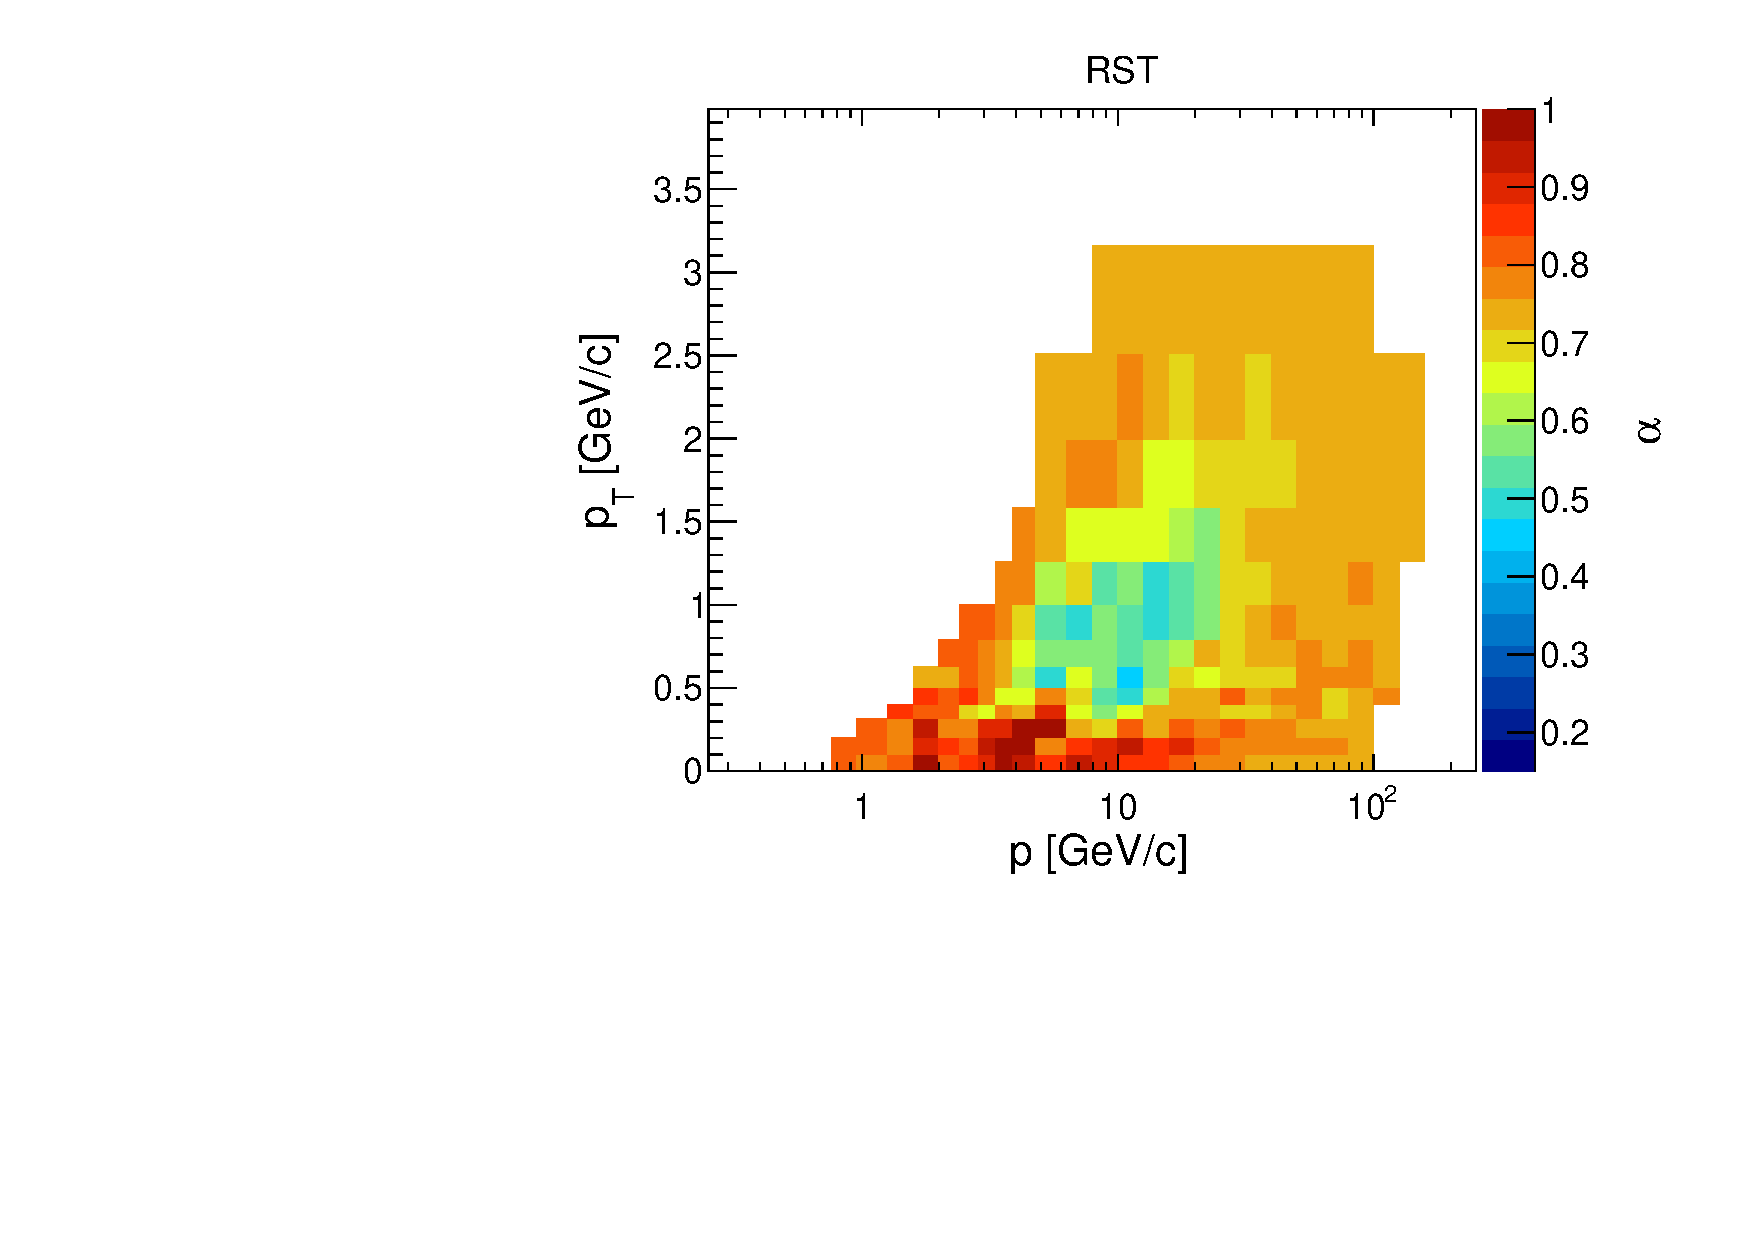
\includegraphics[clip, rviewport=0 0 1 0.94,width=0.4\textwidth]{dedx/model_350_v0_m9}
  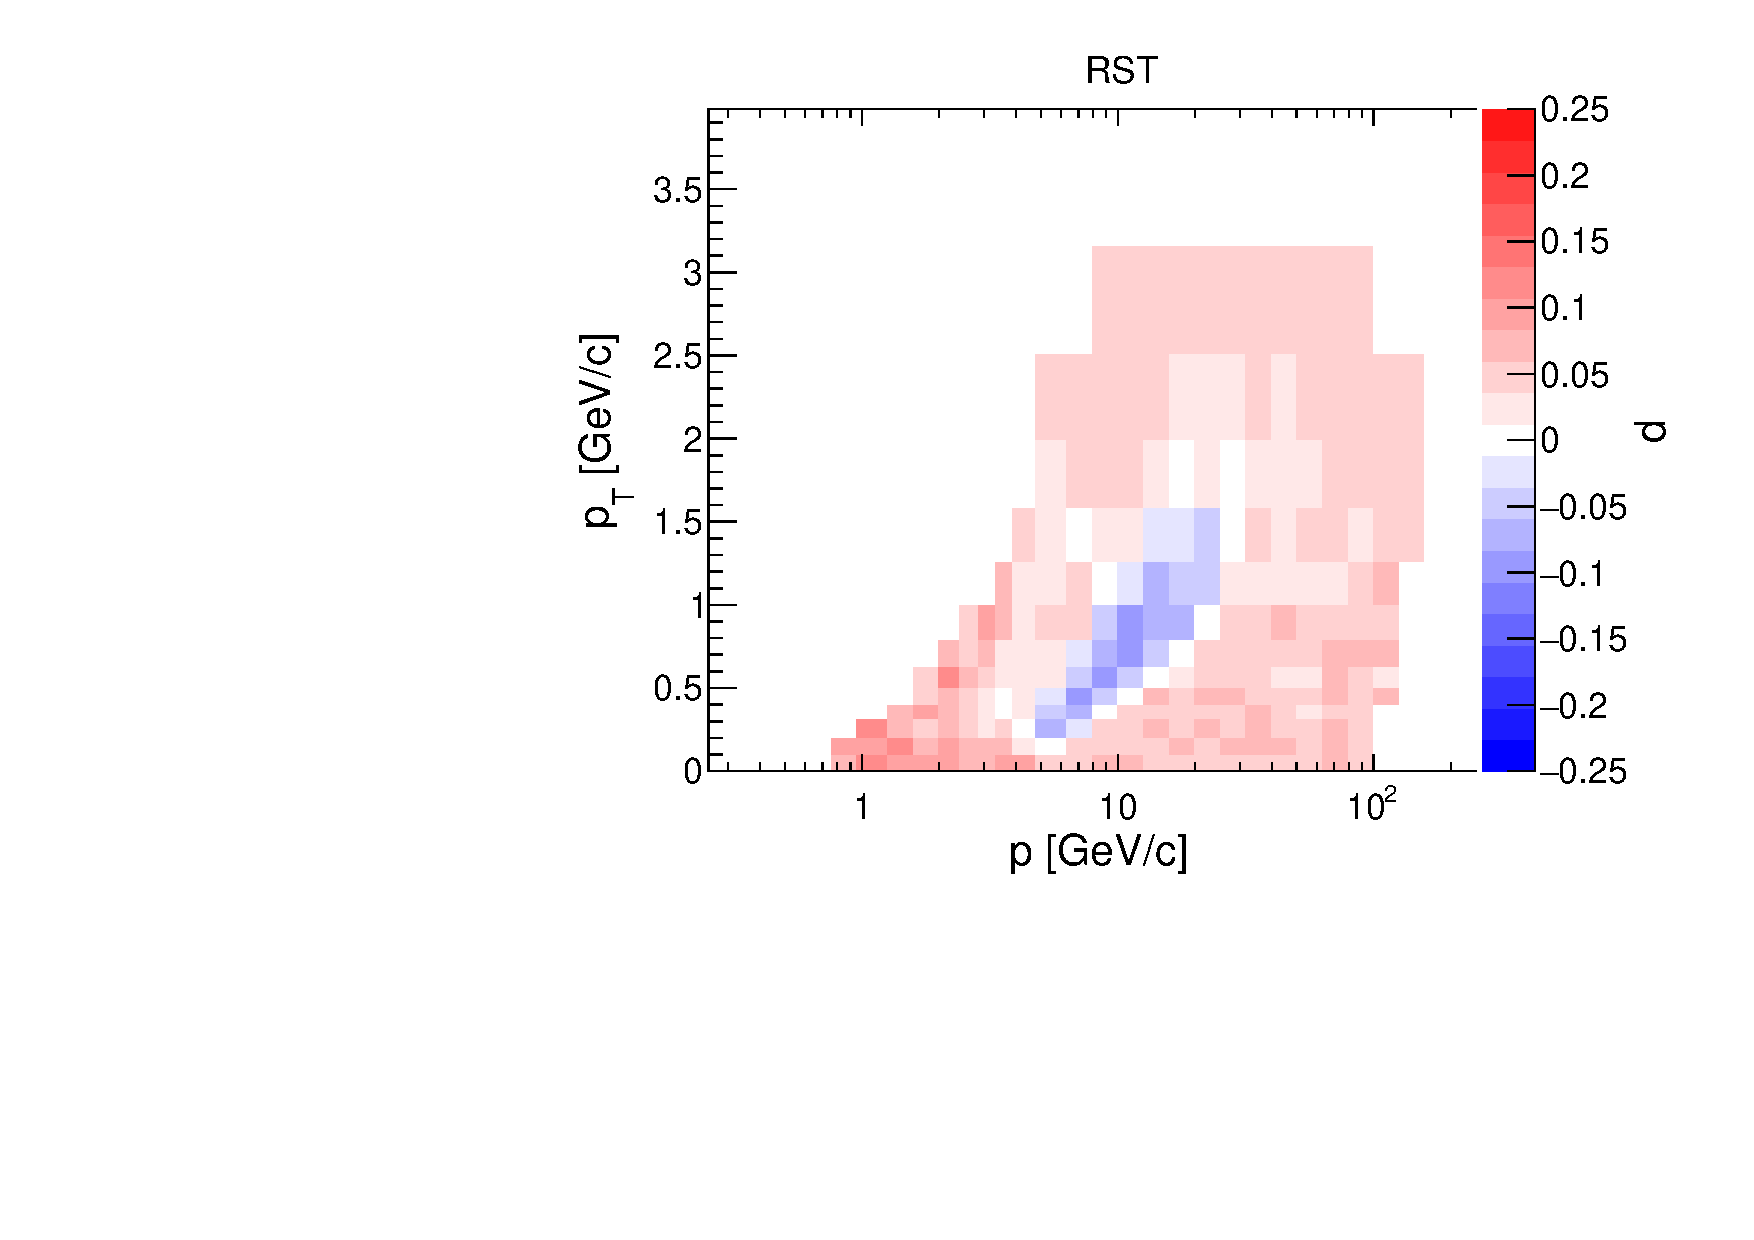
\includegraphics[clip, rviewport=0 0 1 0.94,width=0.4\textwidth]{dedx/model_350_v0_m10}
  \caption{Shape parameters obtained from the fit of the RST dataset at 350 \GeVc.}
  \label{fig:hadron:dedx:fit:shape350r}
\end{figure}

%%%%%%%%%% SHAPE %%%%%%%%%%%%%%
\begin{figure}
  \centering
  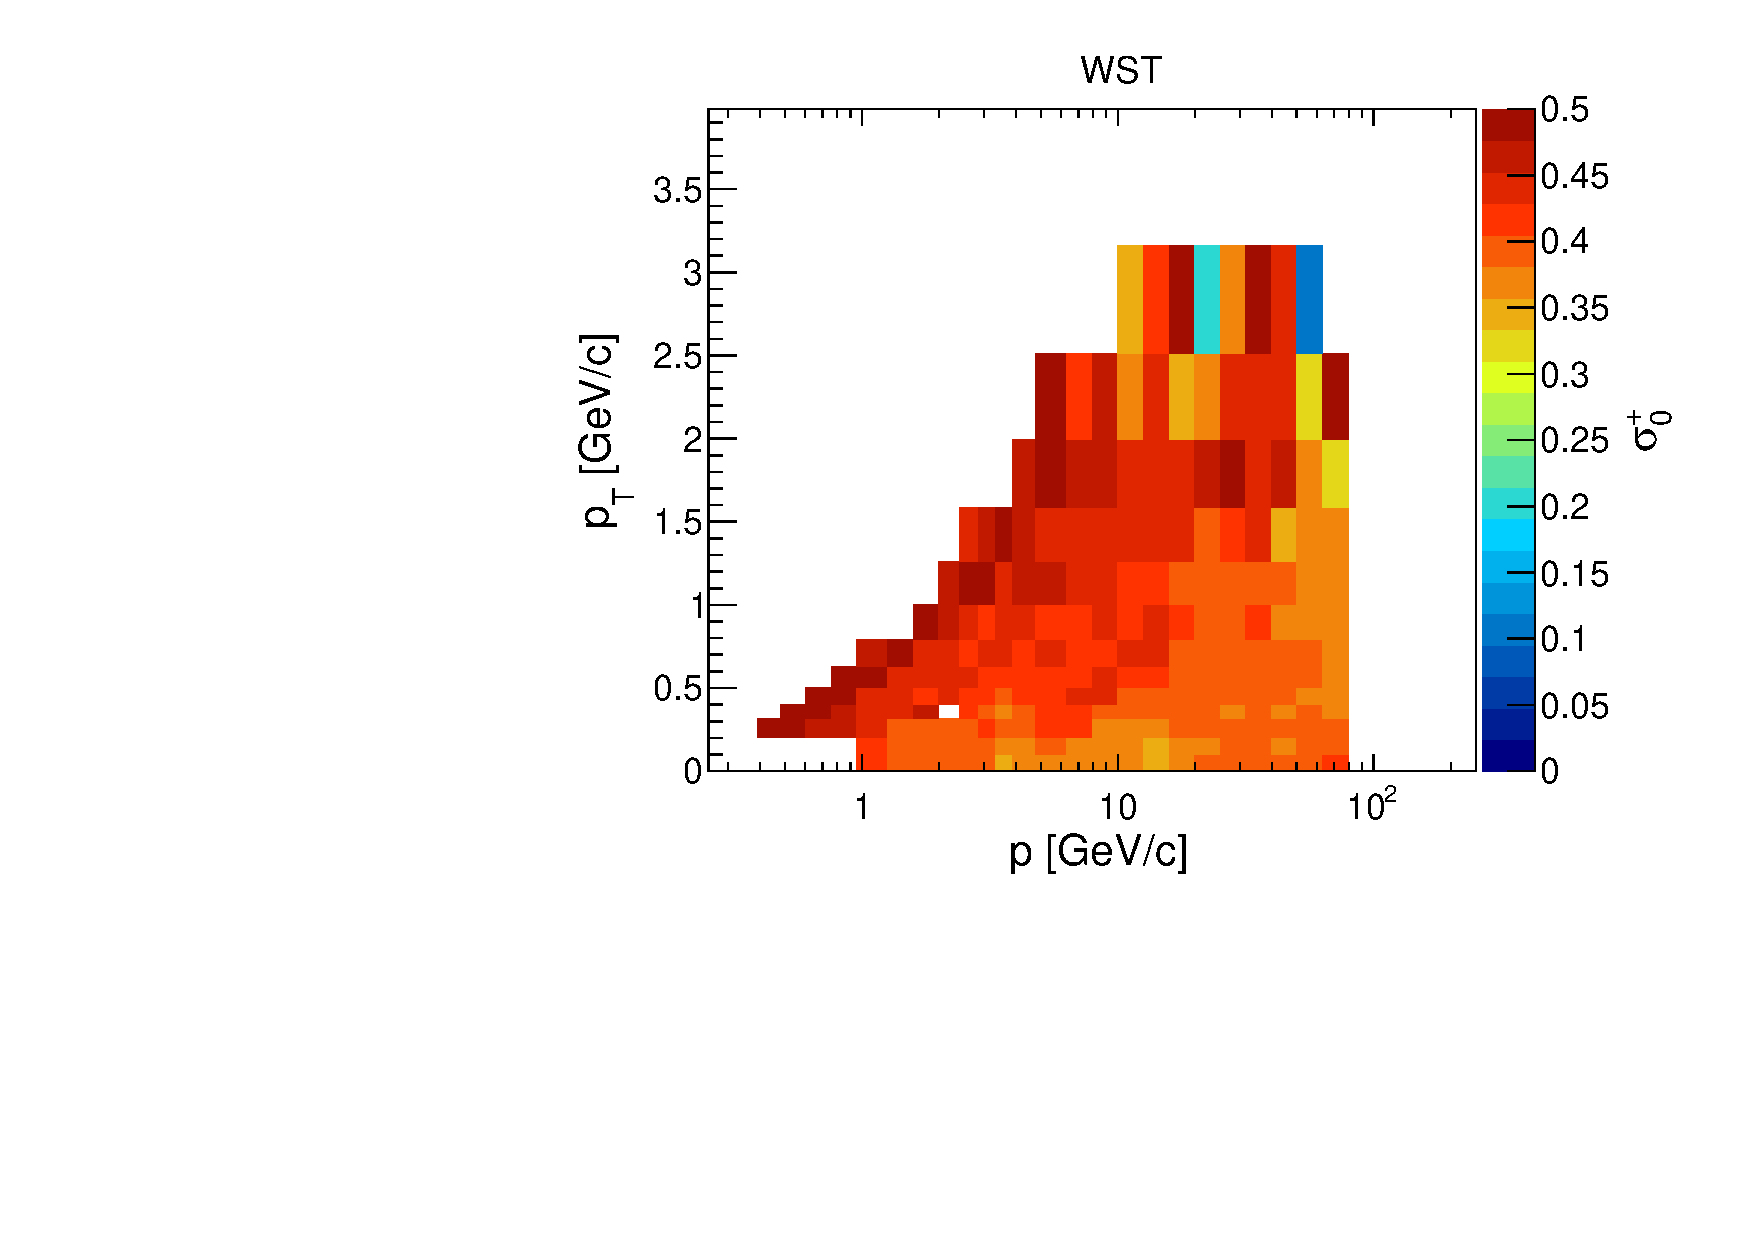
\includegraphics[clip, rviewport=0 0 1 0.94,width=0.4\textwidth]{dedx/model_350_v1_m6}
  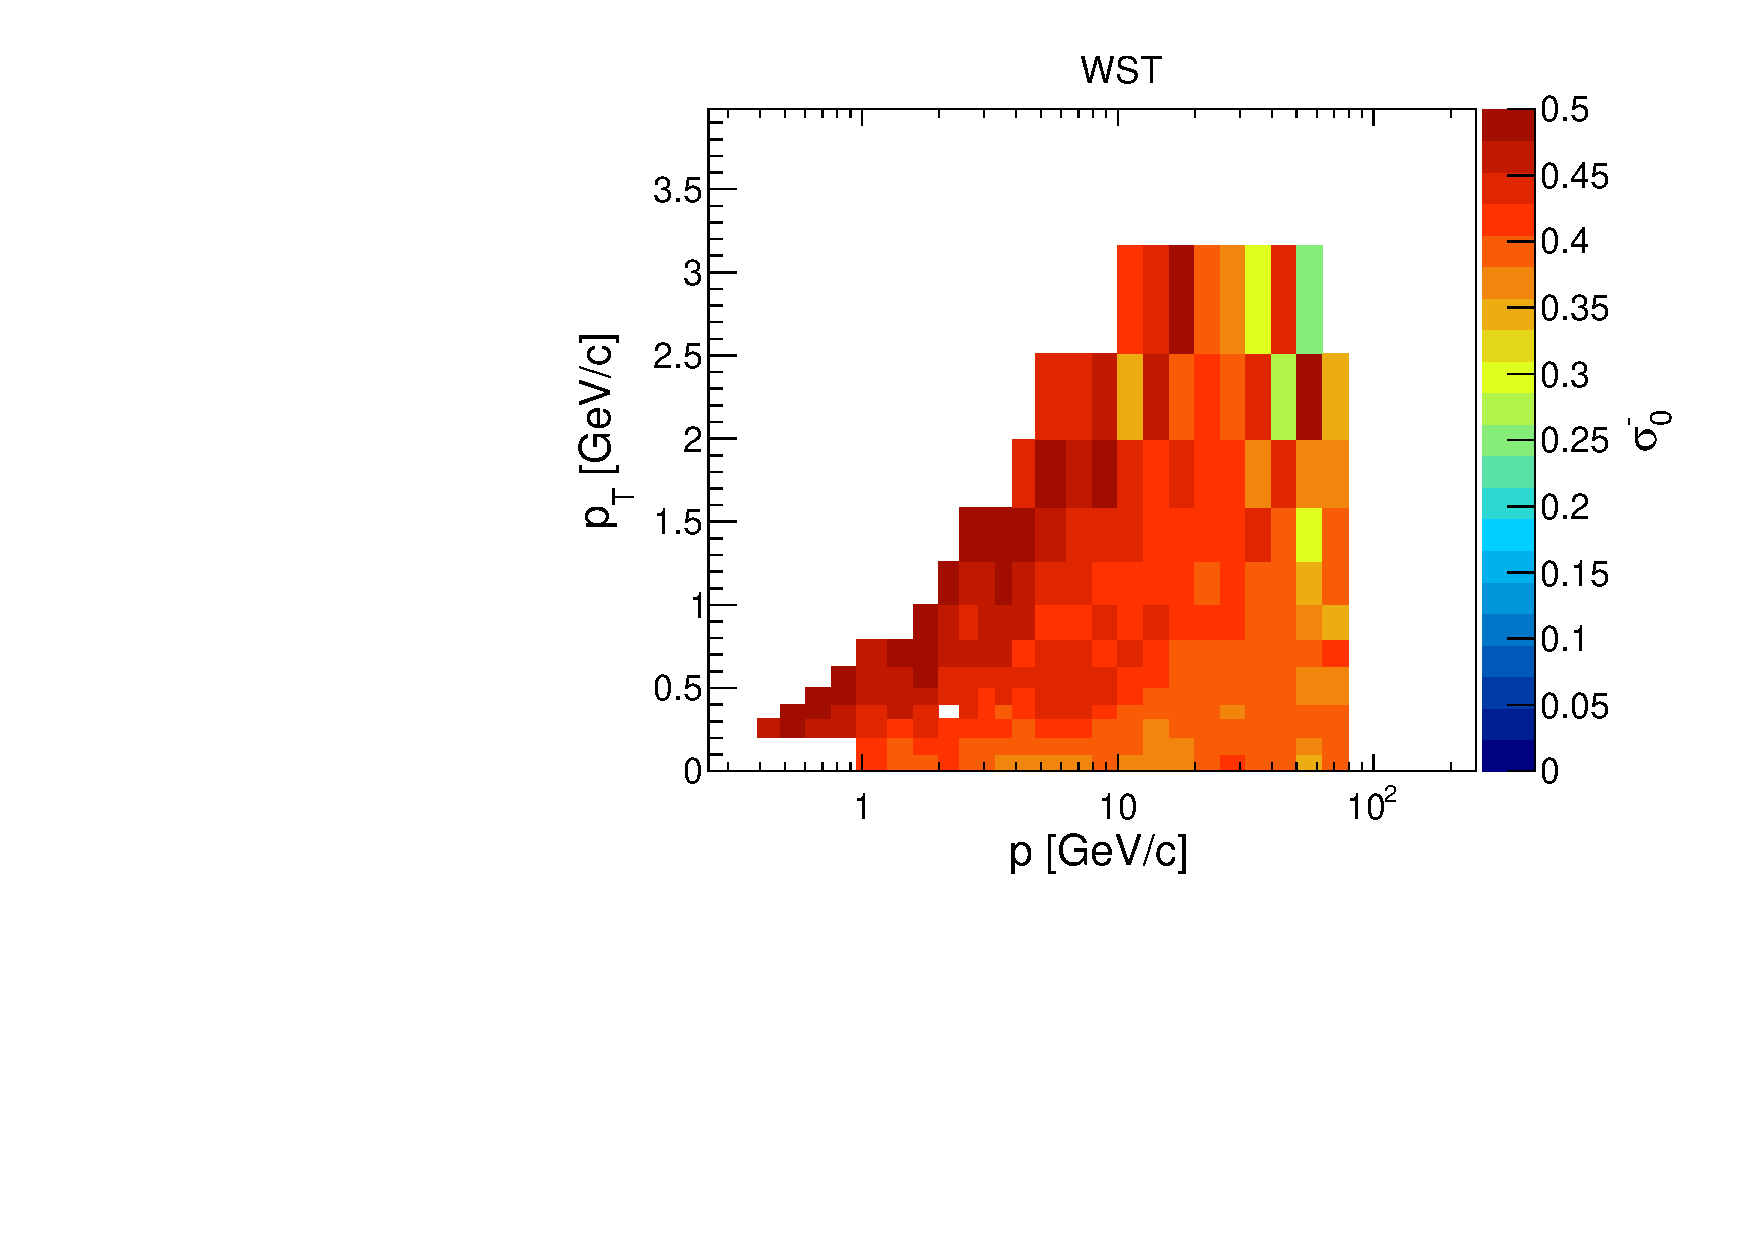
\includegraphics[clip, rviewport=0 0 1 0.94,width=0.4\textwidth]{dedx/model_350_v1_m7}

  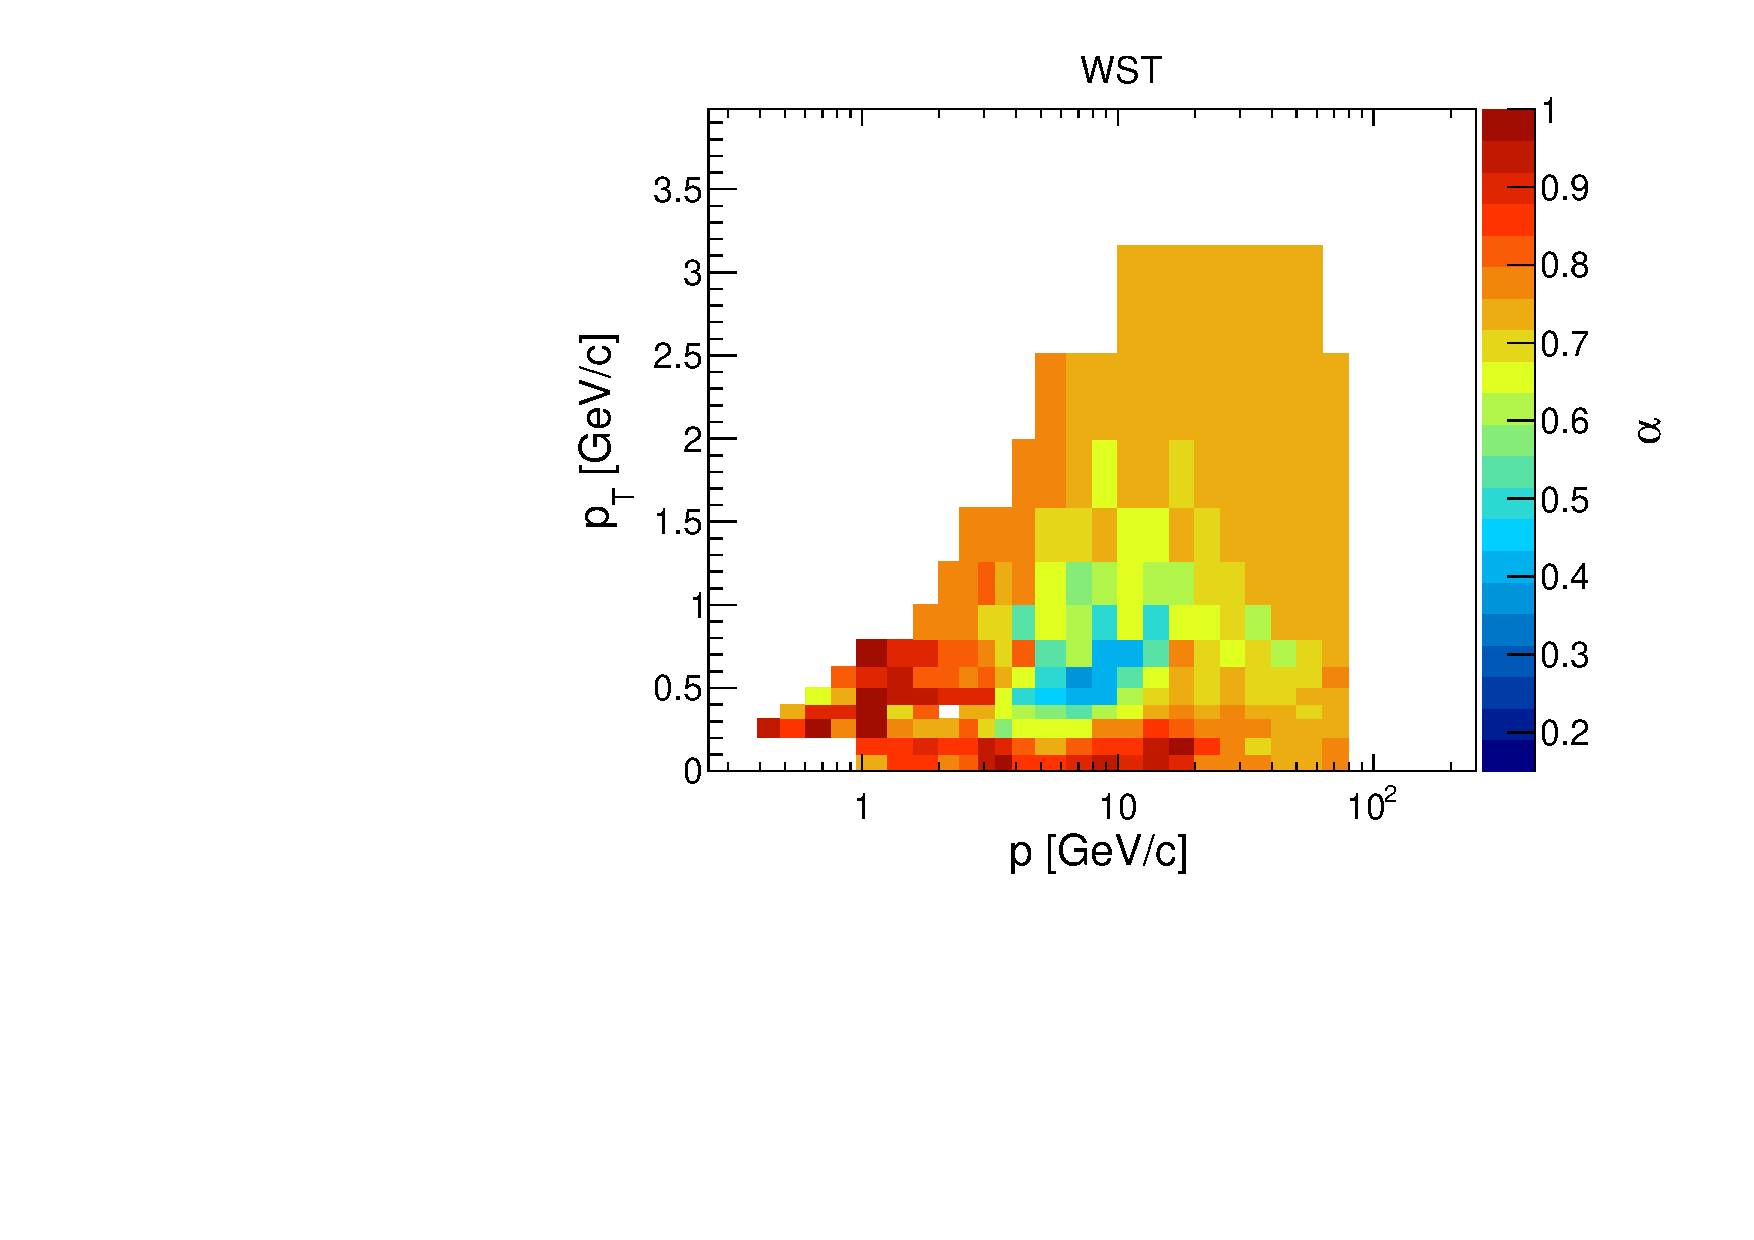
\includegraphics[clip, rviewport=0 0 1 0.94,width=0.4\textwidth]{dedx/model_350_v1_m9}
  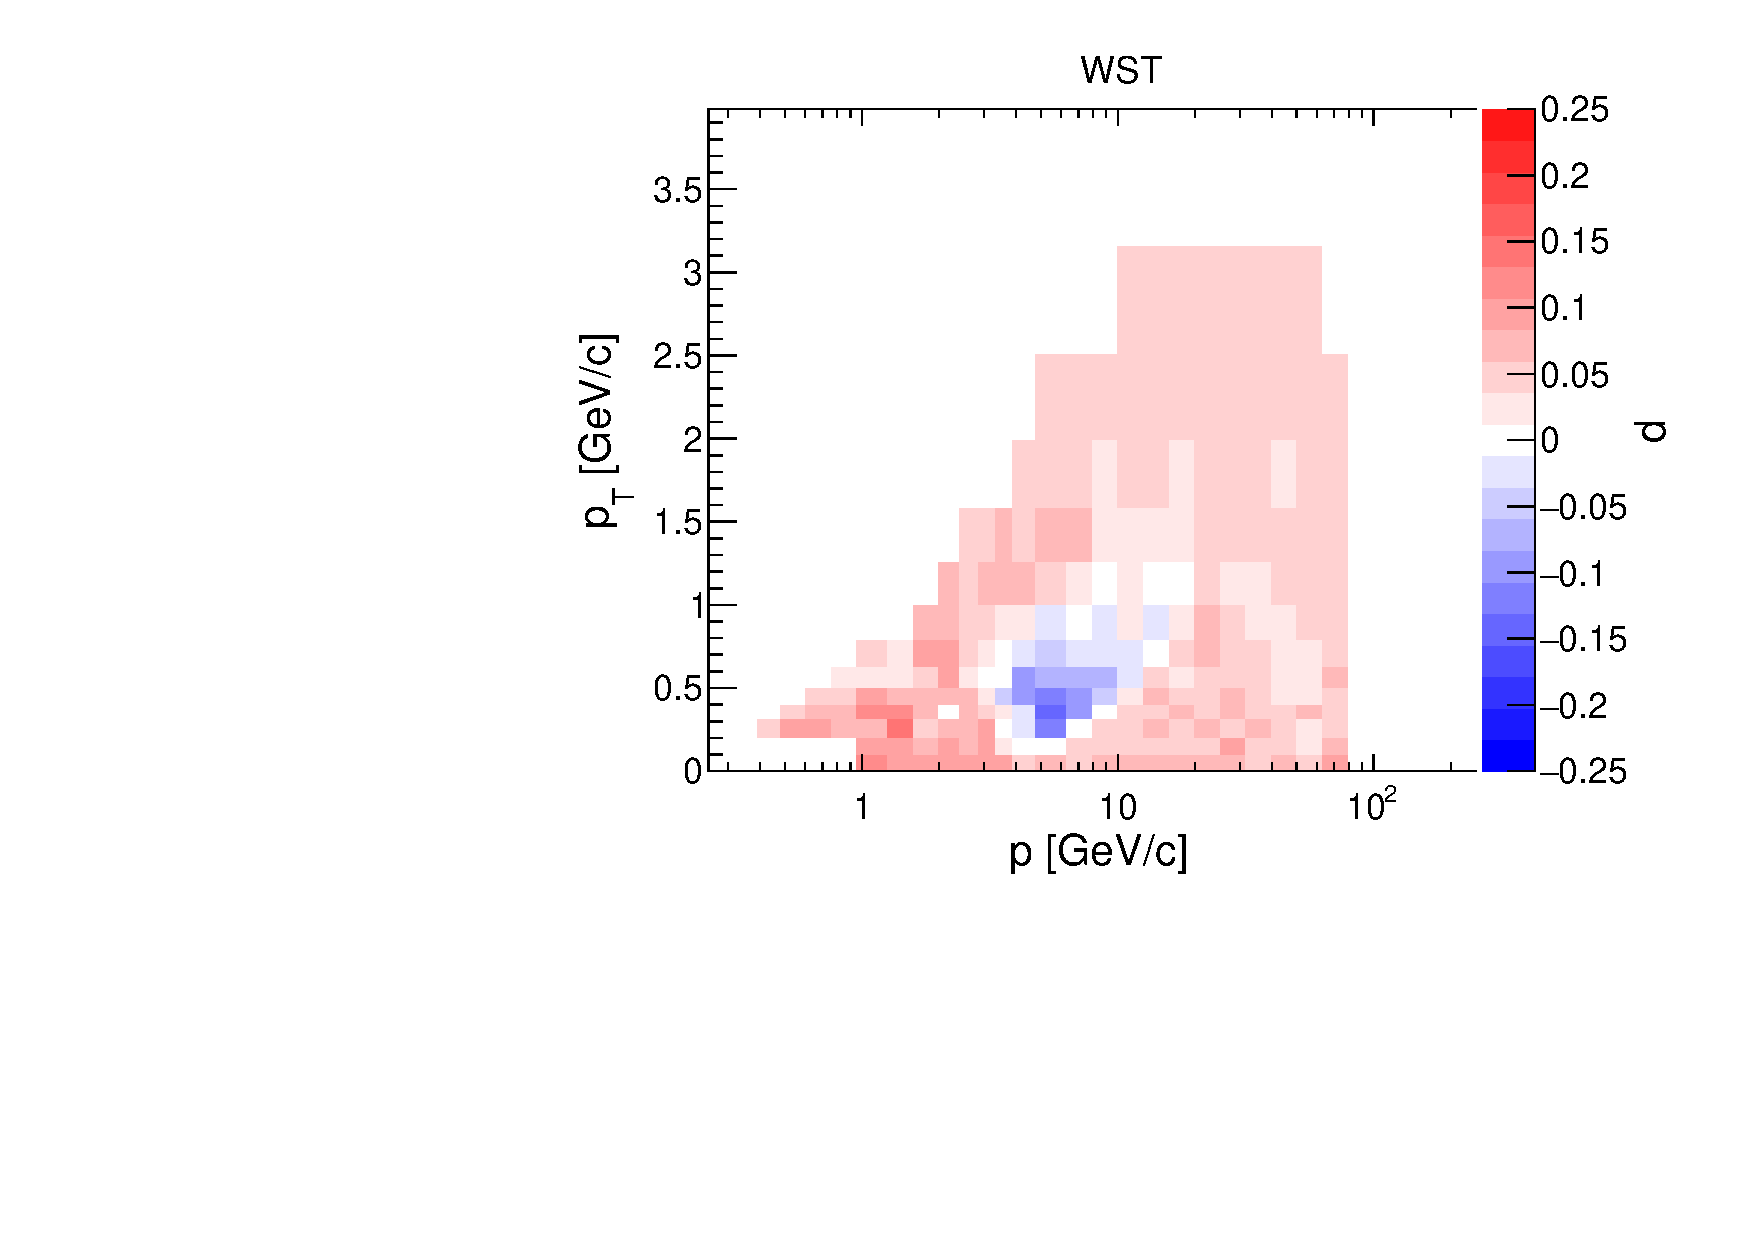
\includegraphics[clip, rviewport=0 0 1 0.94,width=0.4\textwidth]{dedx/model_350_v1_m10}
  \caption{Shape parameters obtained from the fit of the WST dataset at 350 \GeVc.}
  \label{fig:hadron:dedx:fit:shape350w}
\end{figure}

\clearpage


%%%%%%%%%% FRACTIONS %%%%%%%%%%%%%%
\begin{figure}
  \centering
  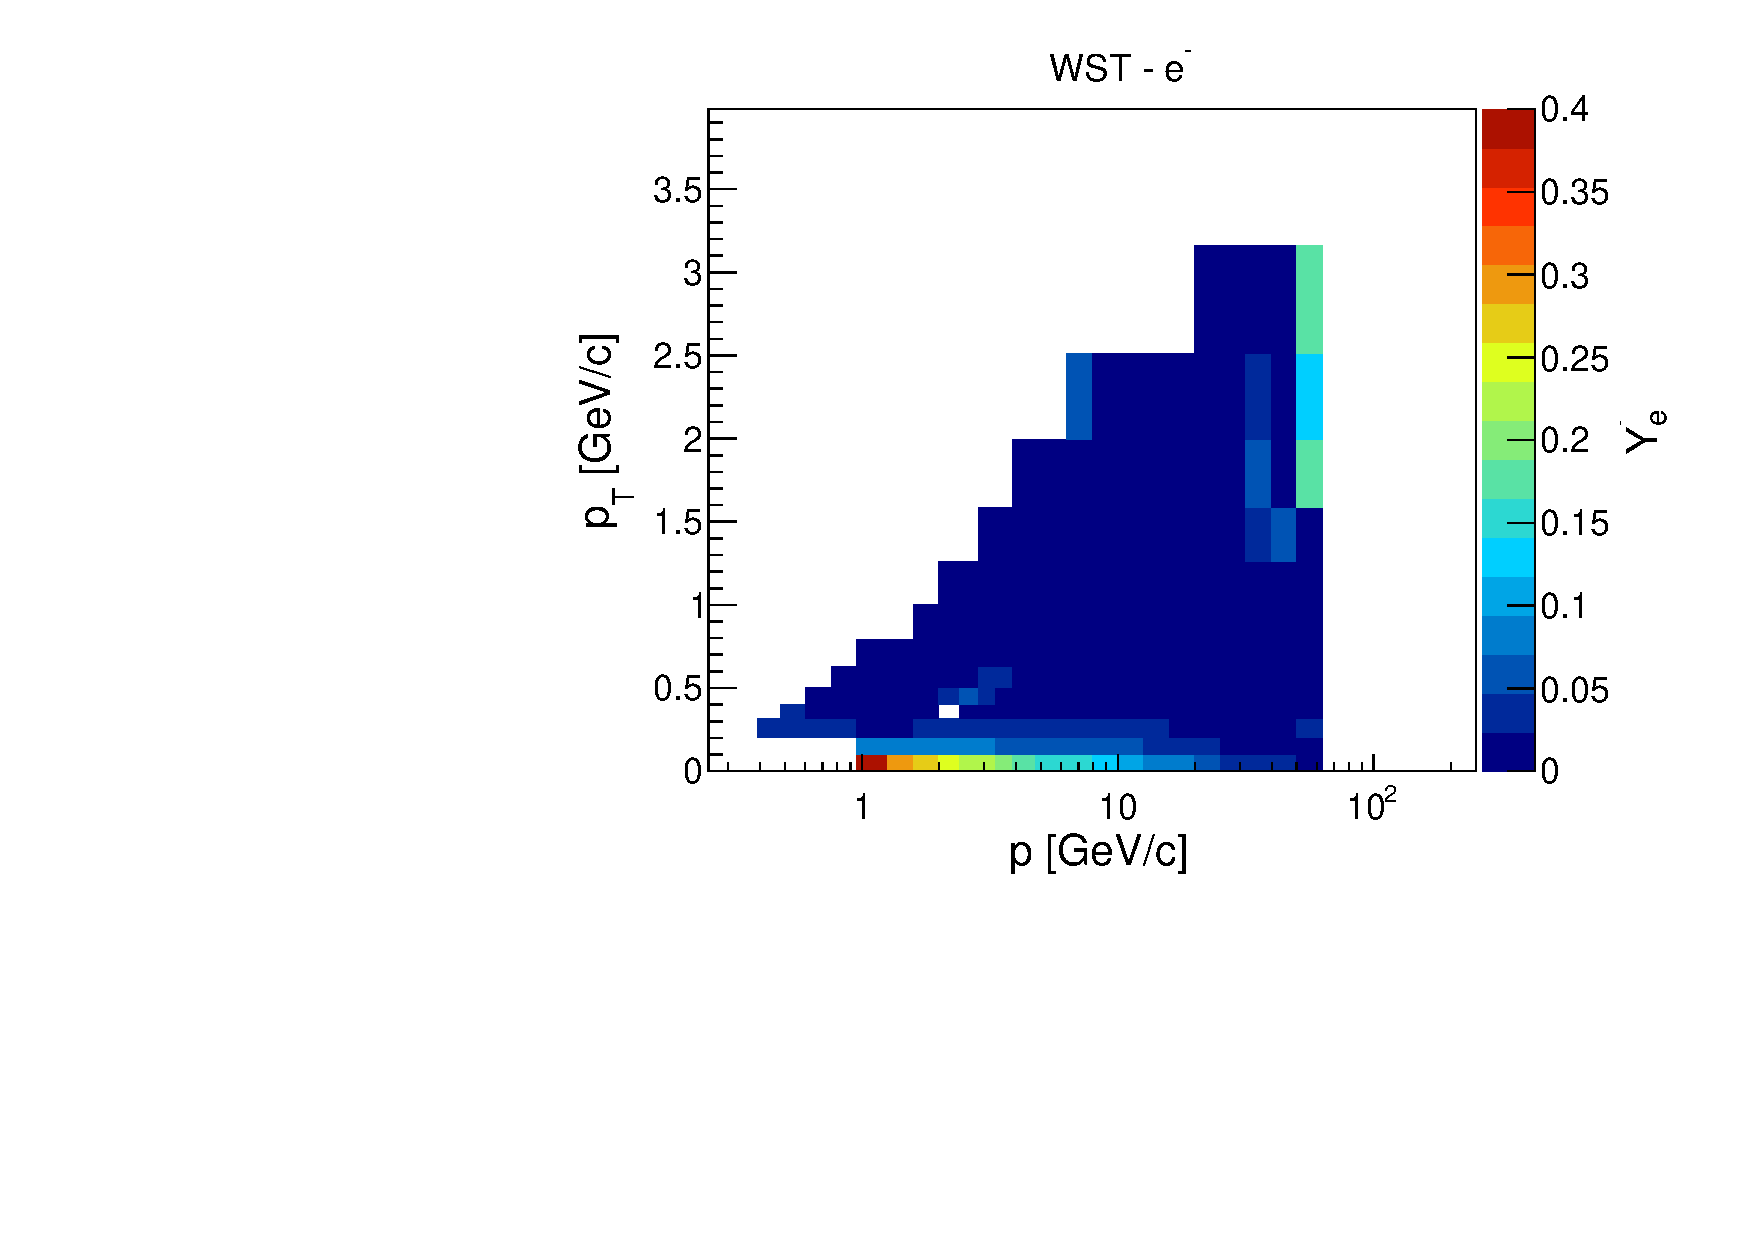
\includegraphics[clip, rviewport=0 0.13 1 0.94,width=0.4\textwidth]{dedx/fraction_158_fl0_v1_c0_p0}
  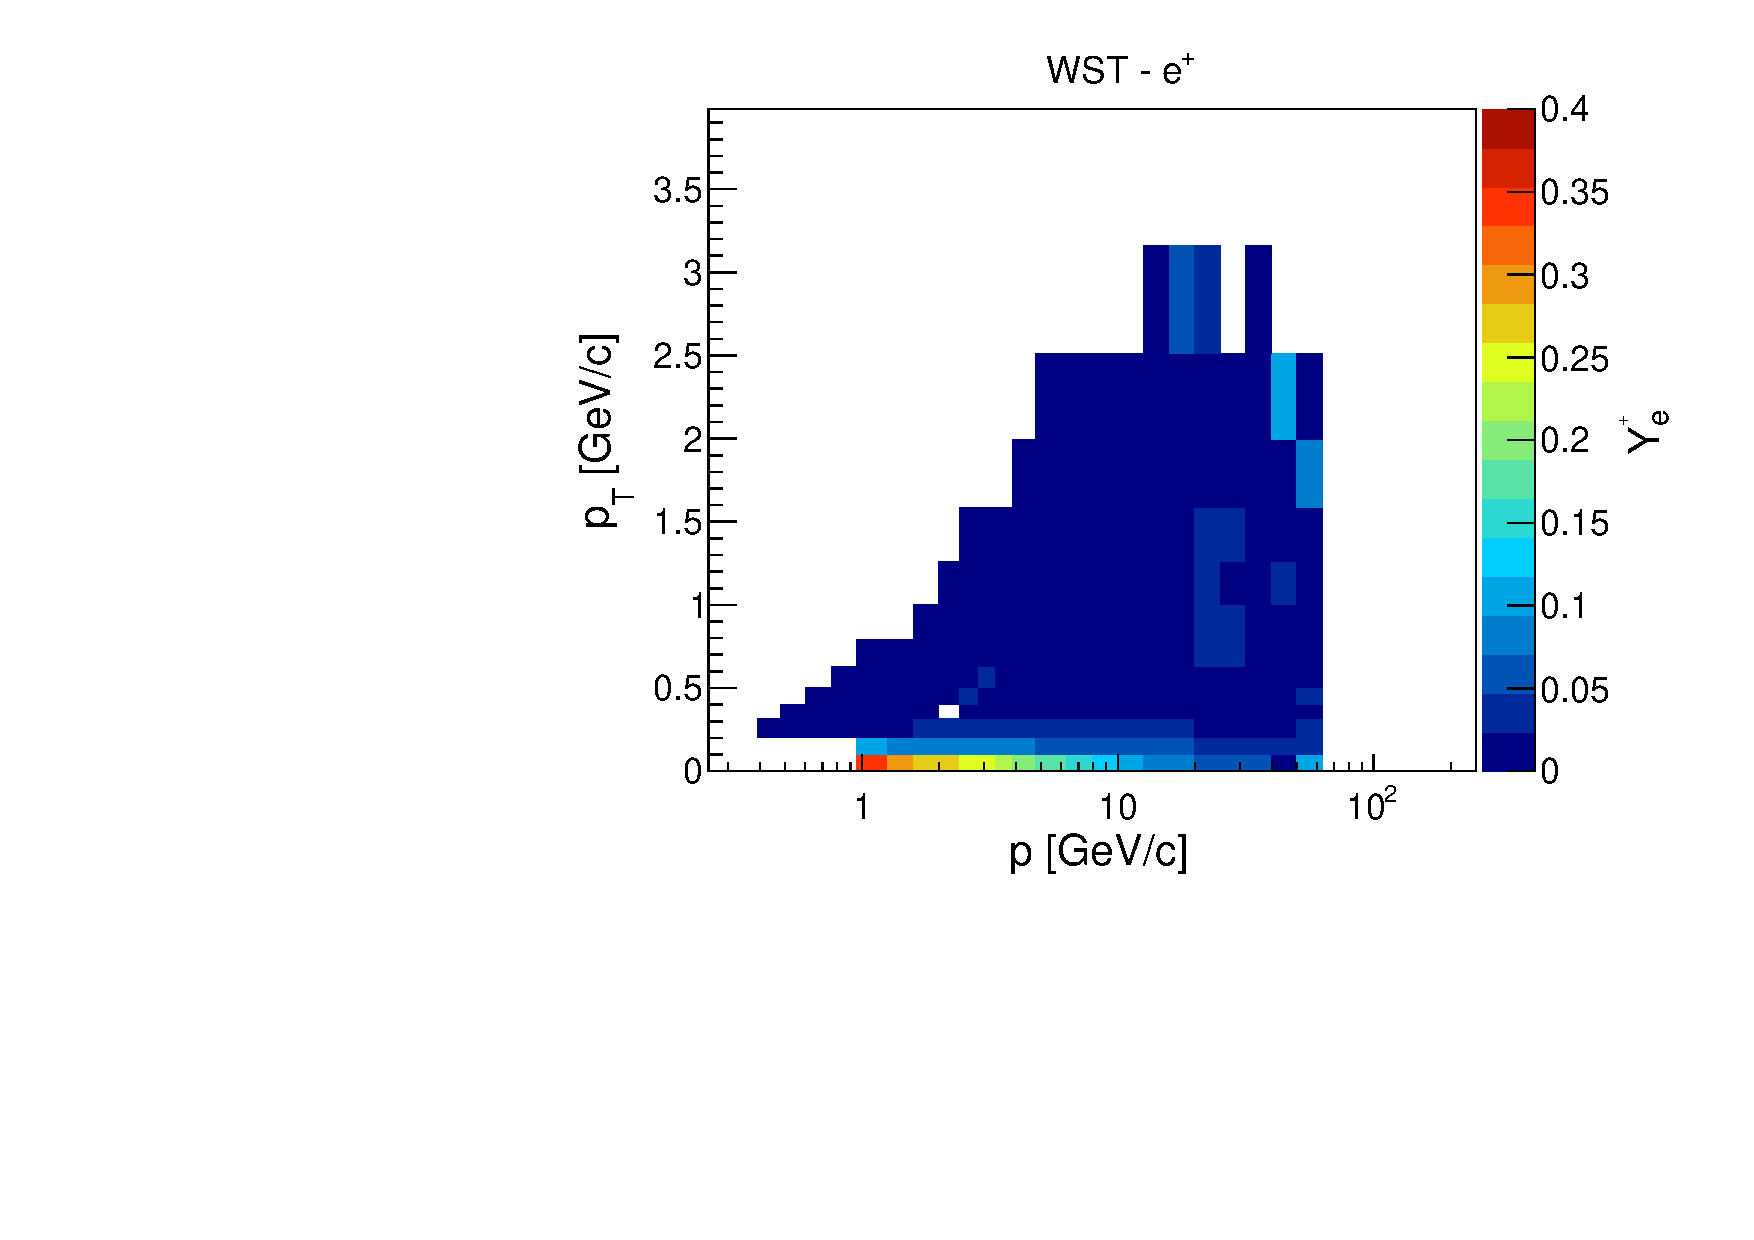
\includegraphics[clip, rviewport=0 0.13 1 0.94,width=0.4\textwidth]{dedx/fraction_158_fl0_v1_c1_p0}

  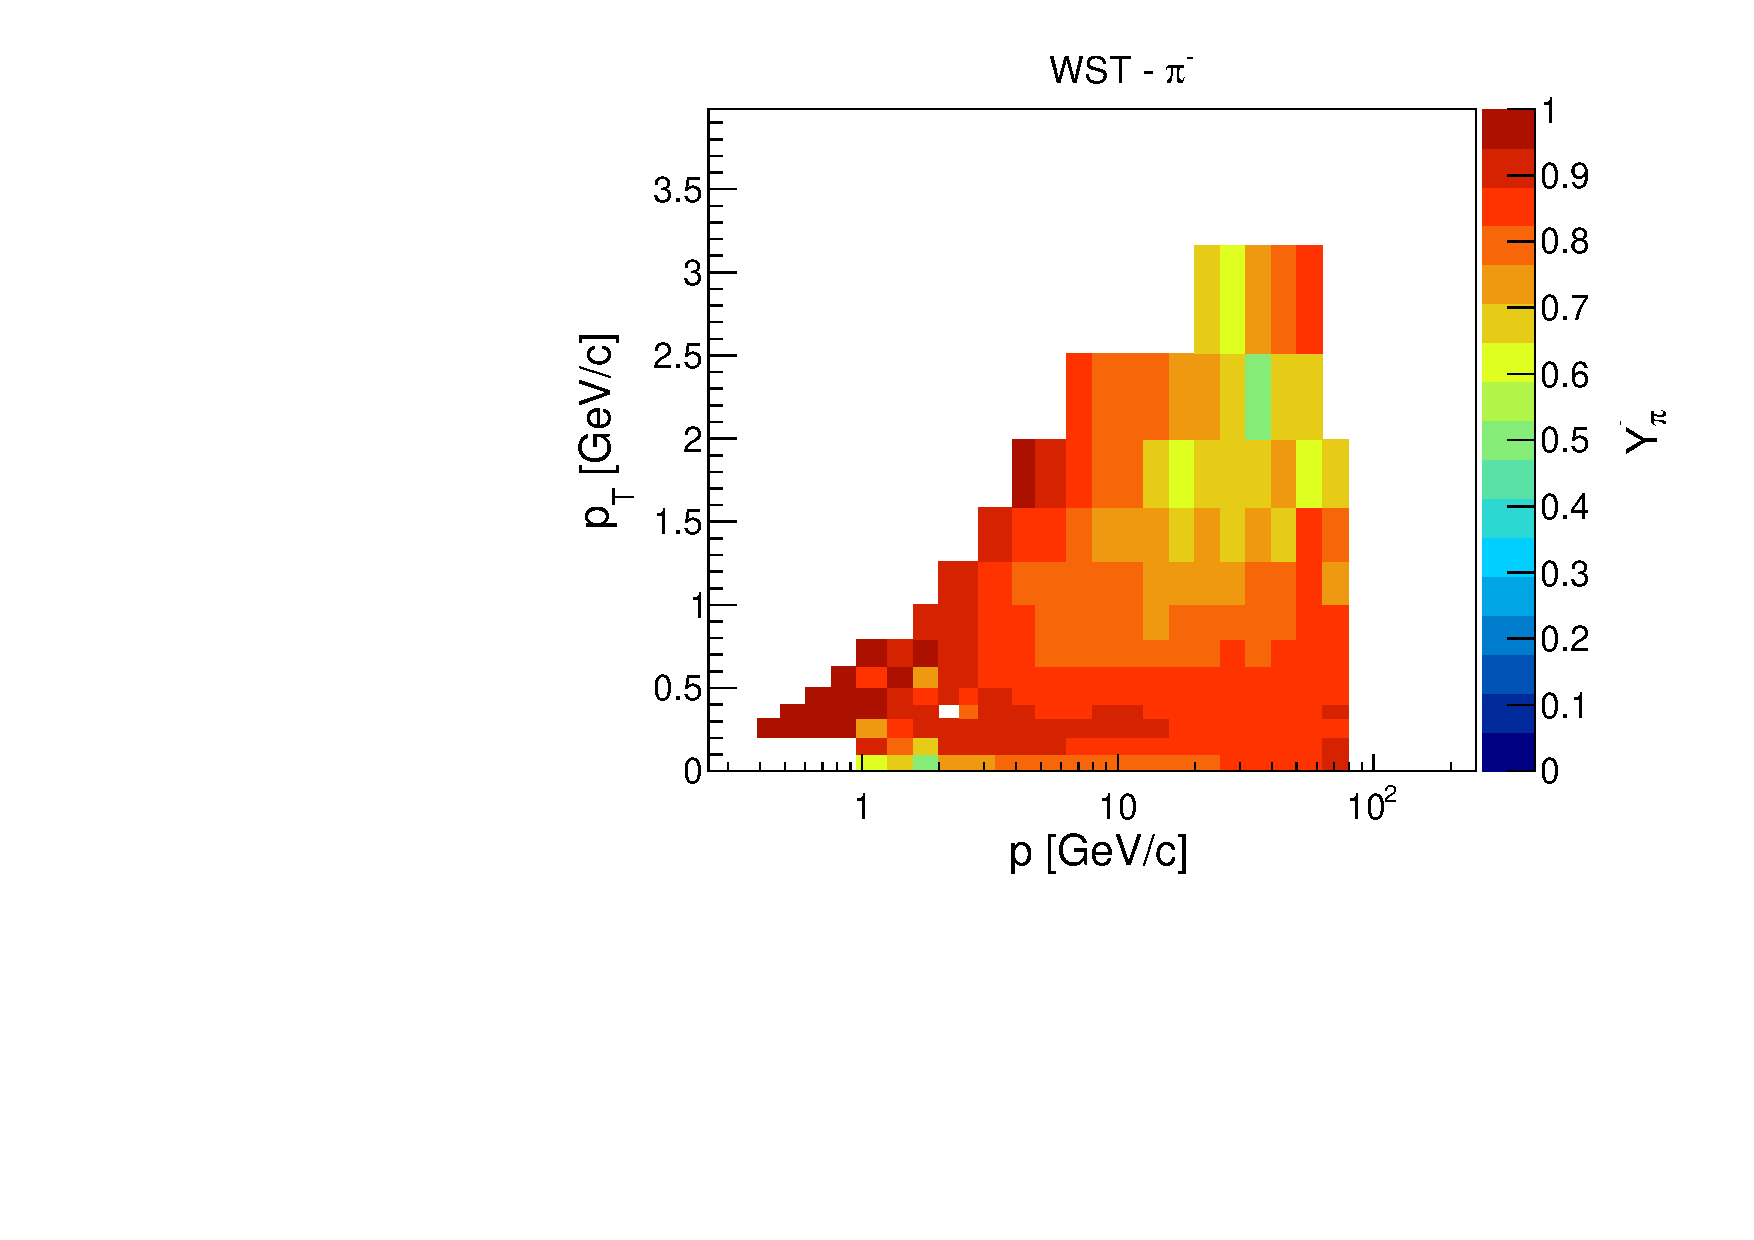
\includegraphics[clip, rviewport=0 0.13 1 0.94,width=0.4\textwidth]{dedx/fraction_158_fl0_v1_c0_p1}
  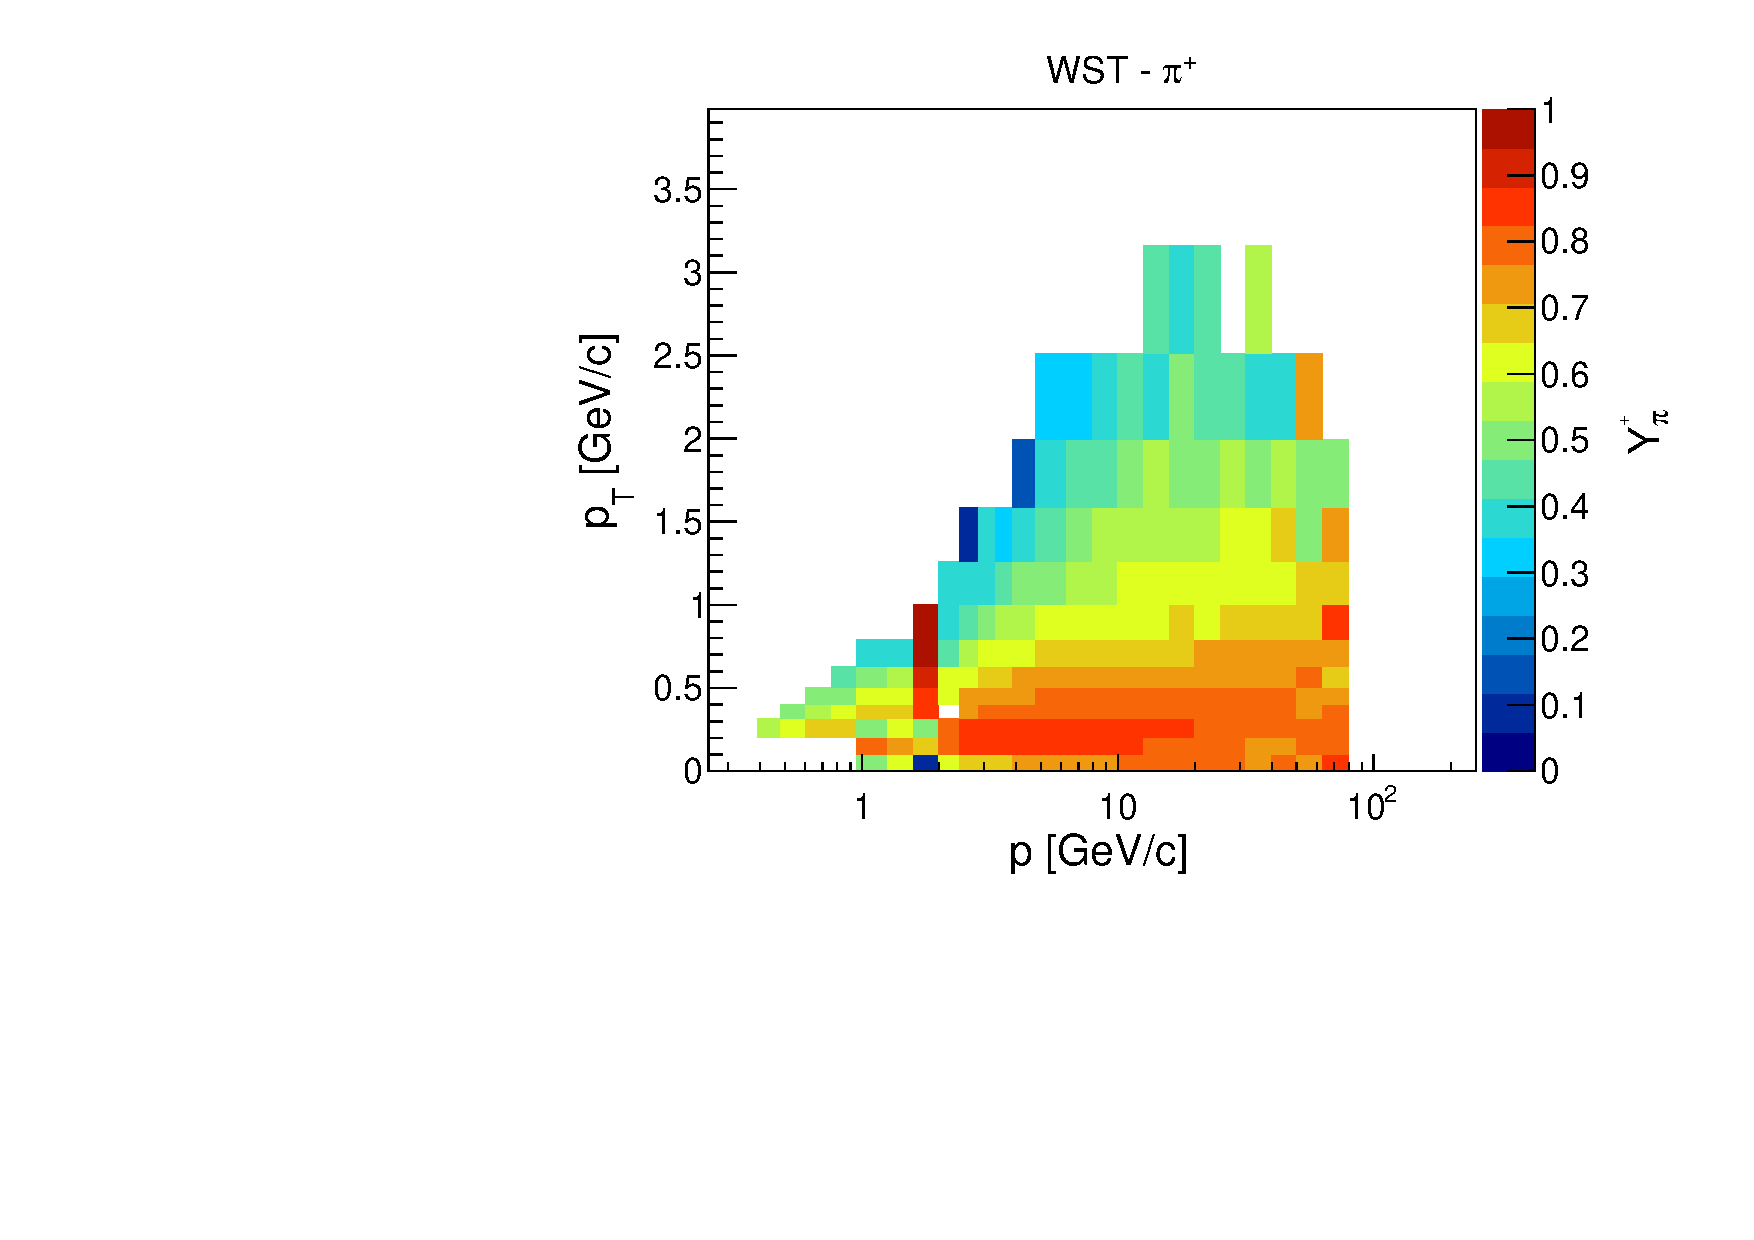
\includegraphics[clip, rviewport=0 0.13 1 0.94,width=0.4\textwidth]{dedx/fraction_158_fl0_v1_c1_p1}

  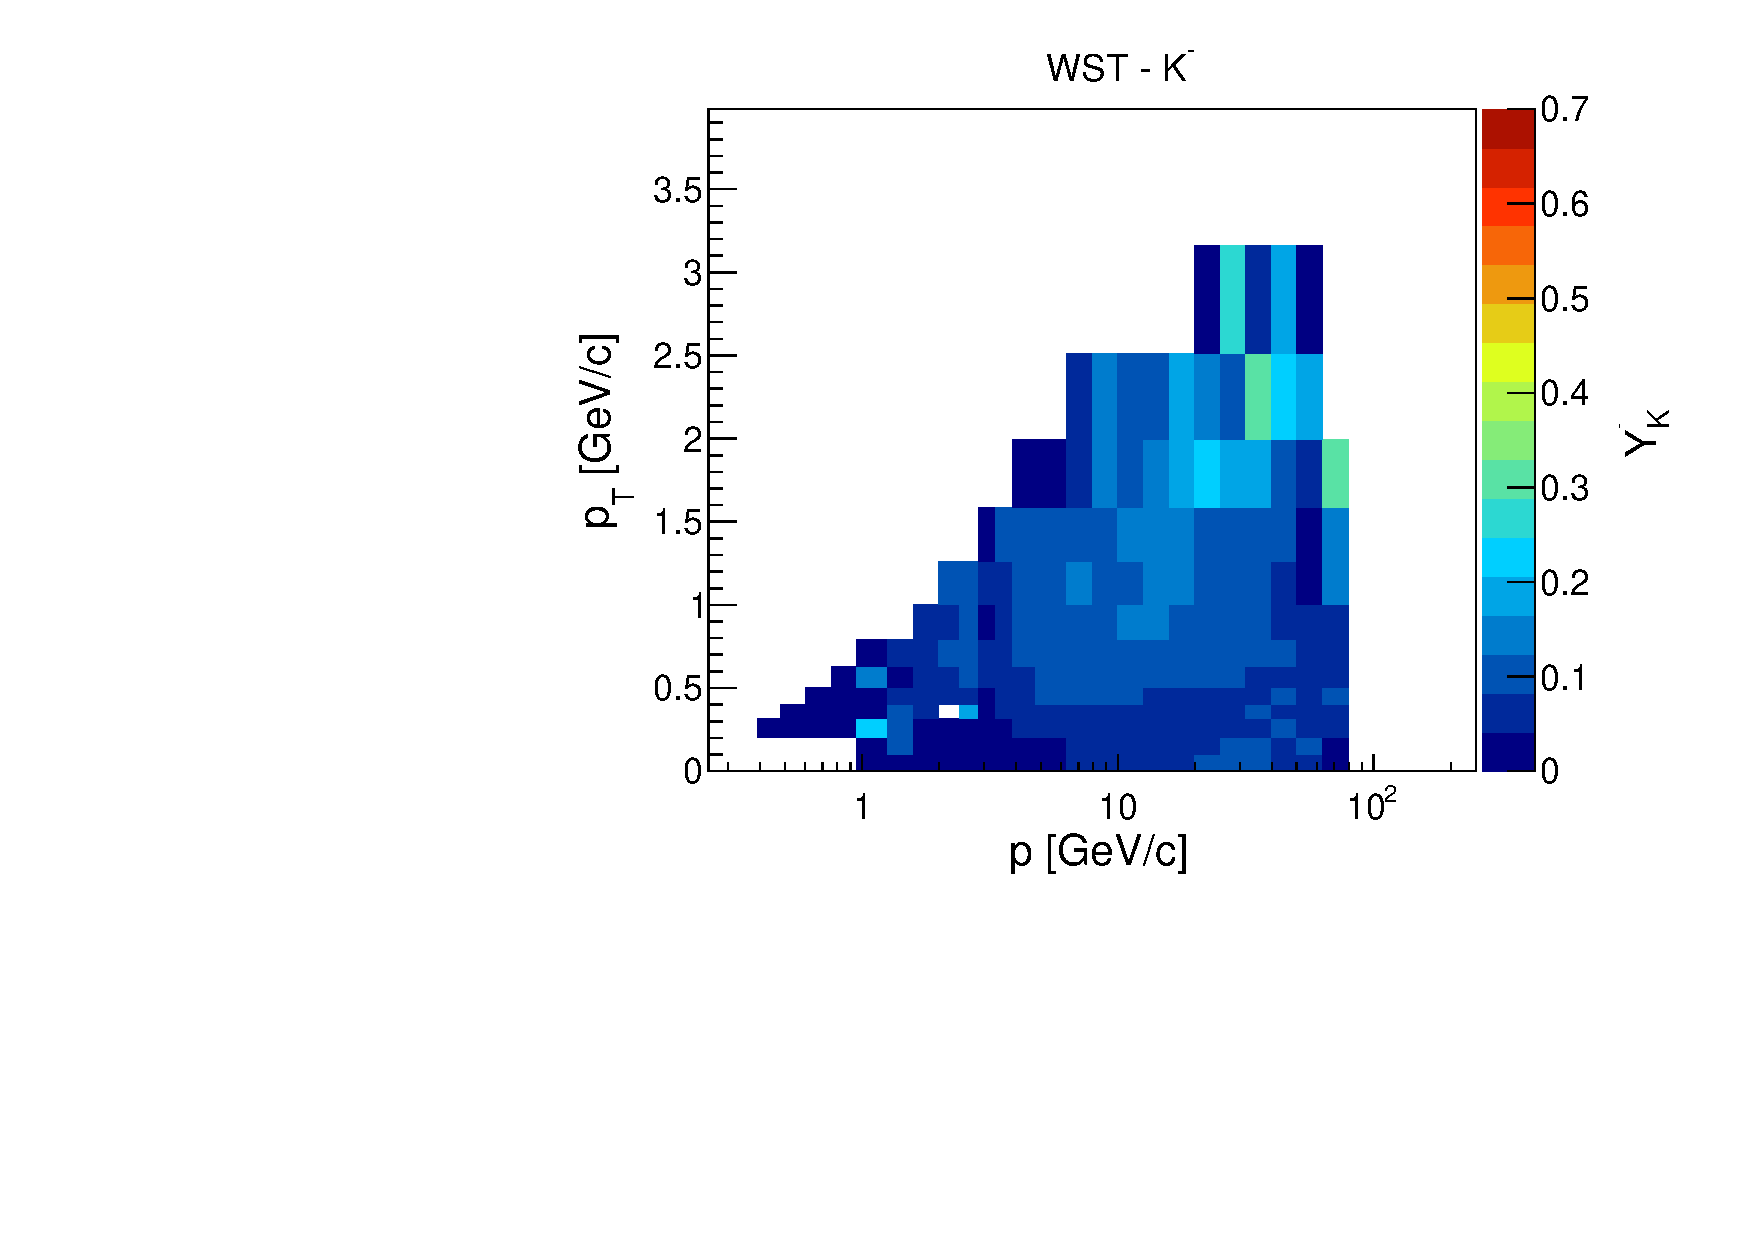
\includegraphics[clip, rviewport=0 0.13 1 0.94,width=0.4\textwidth]{dedx/fraction_158_fl0_v1_c0_p2}
  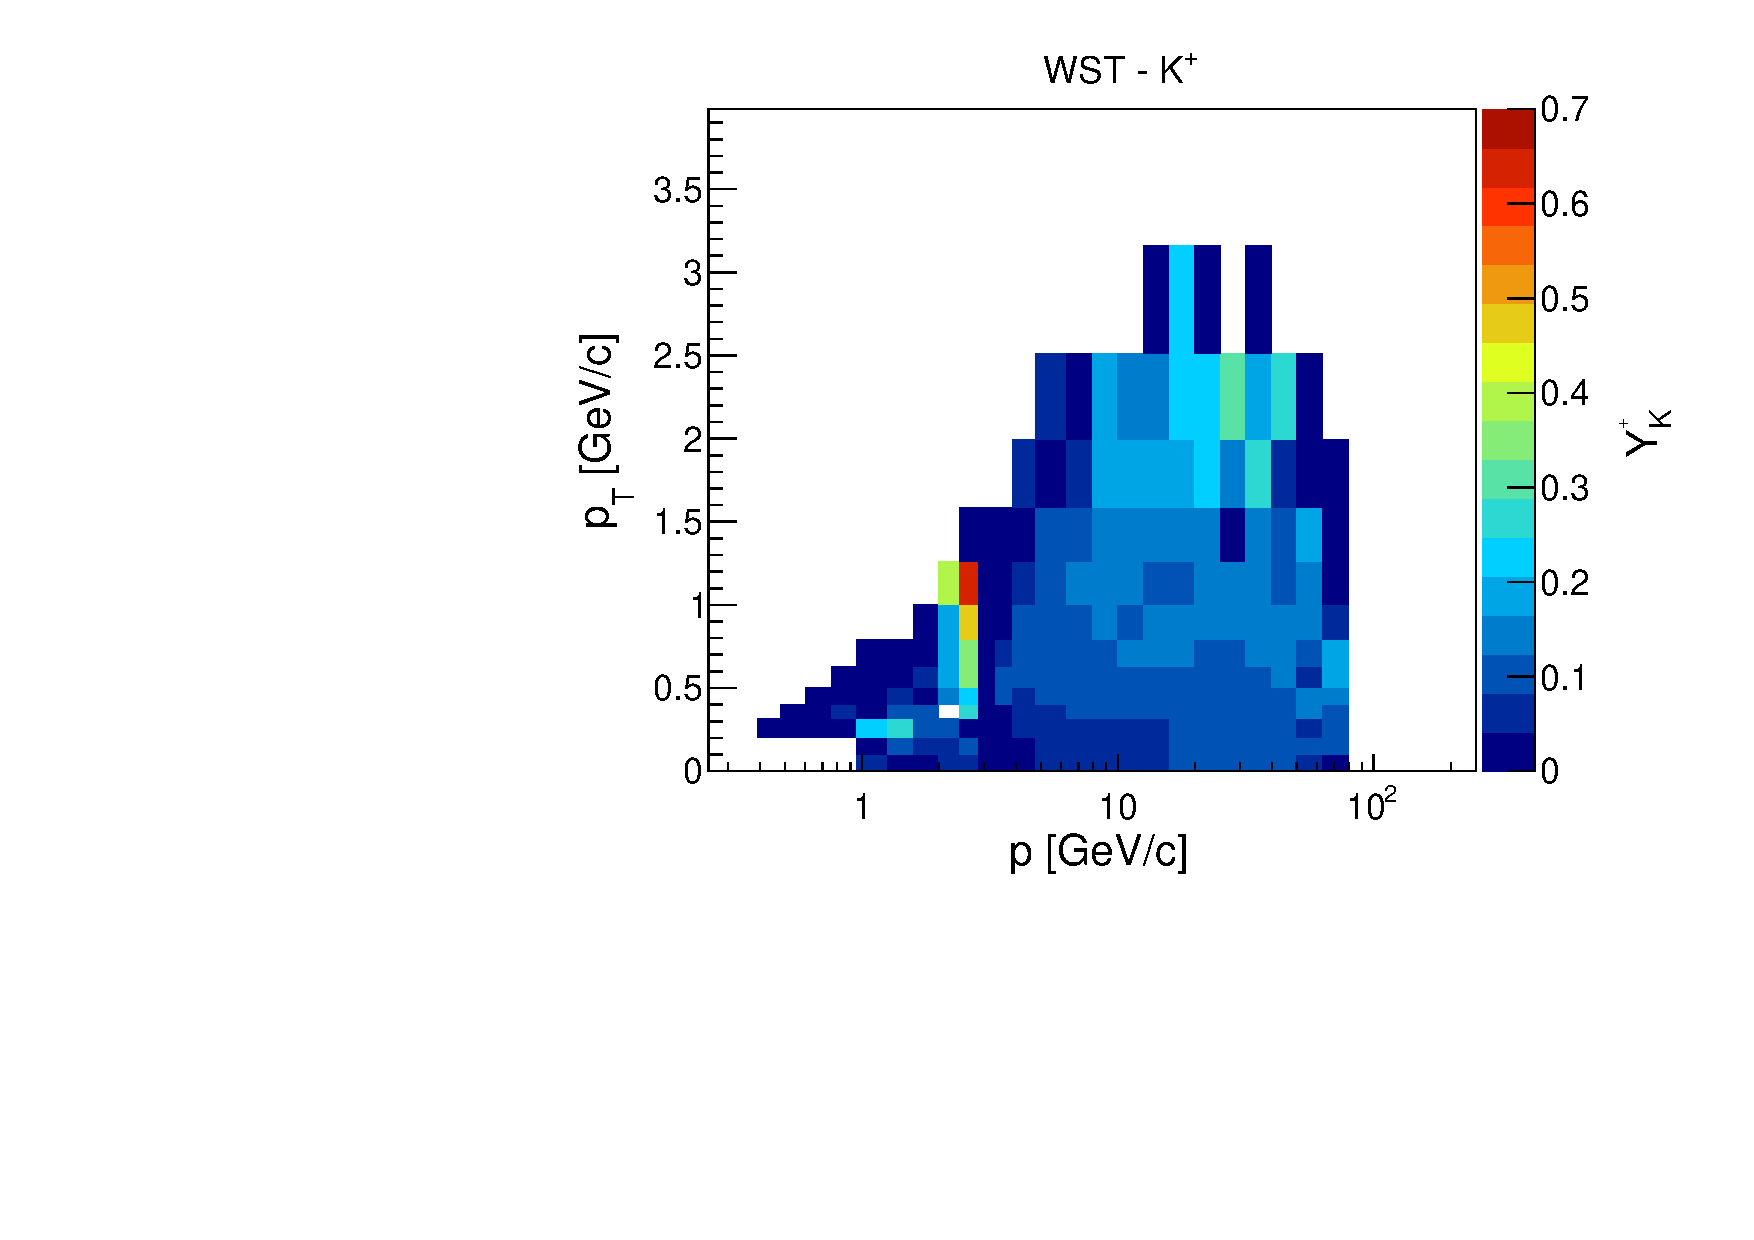
\includegraphics[clip, rviewport=0 0.13 1 0.94,width=0.4\textwidth]{dedx/fraction_158_fl0_v1_c1_p2}


  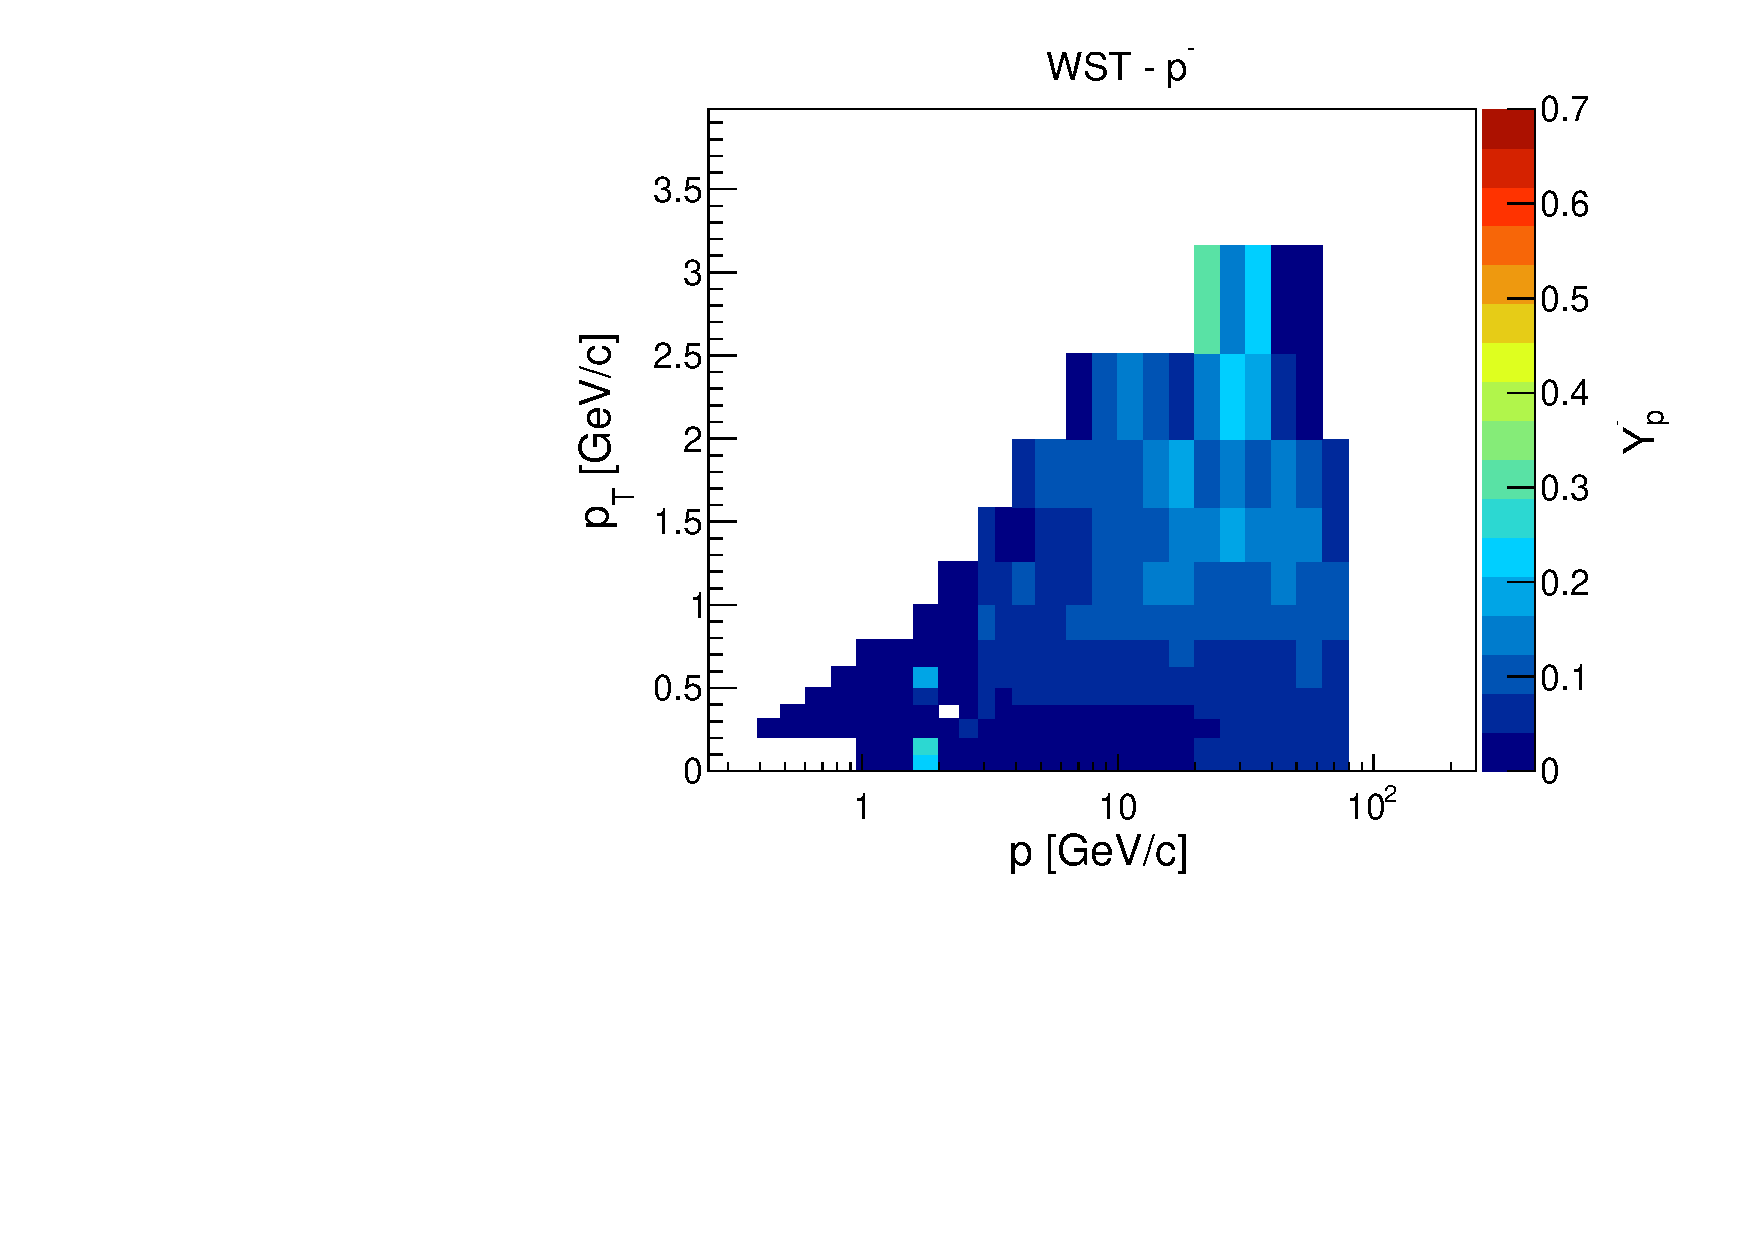
\includegraphics[clip, rviewport=0 0.13 1 0.94,width=0.4\textwidth]{dedx/fraction_158_fl0_v1_c0_p3}
  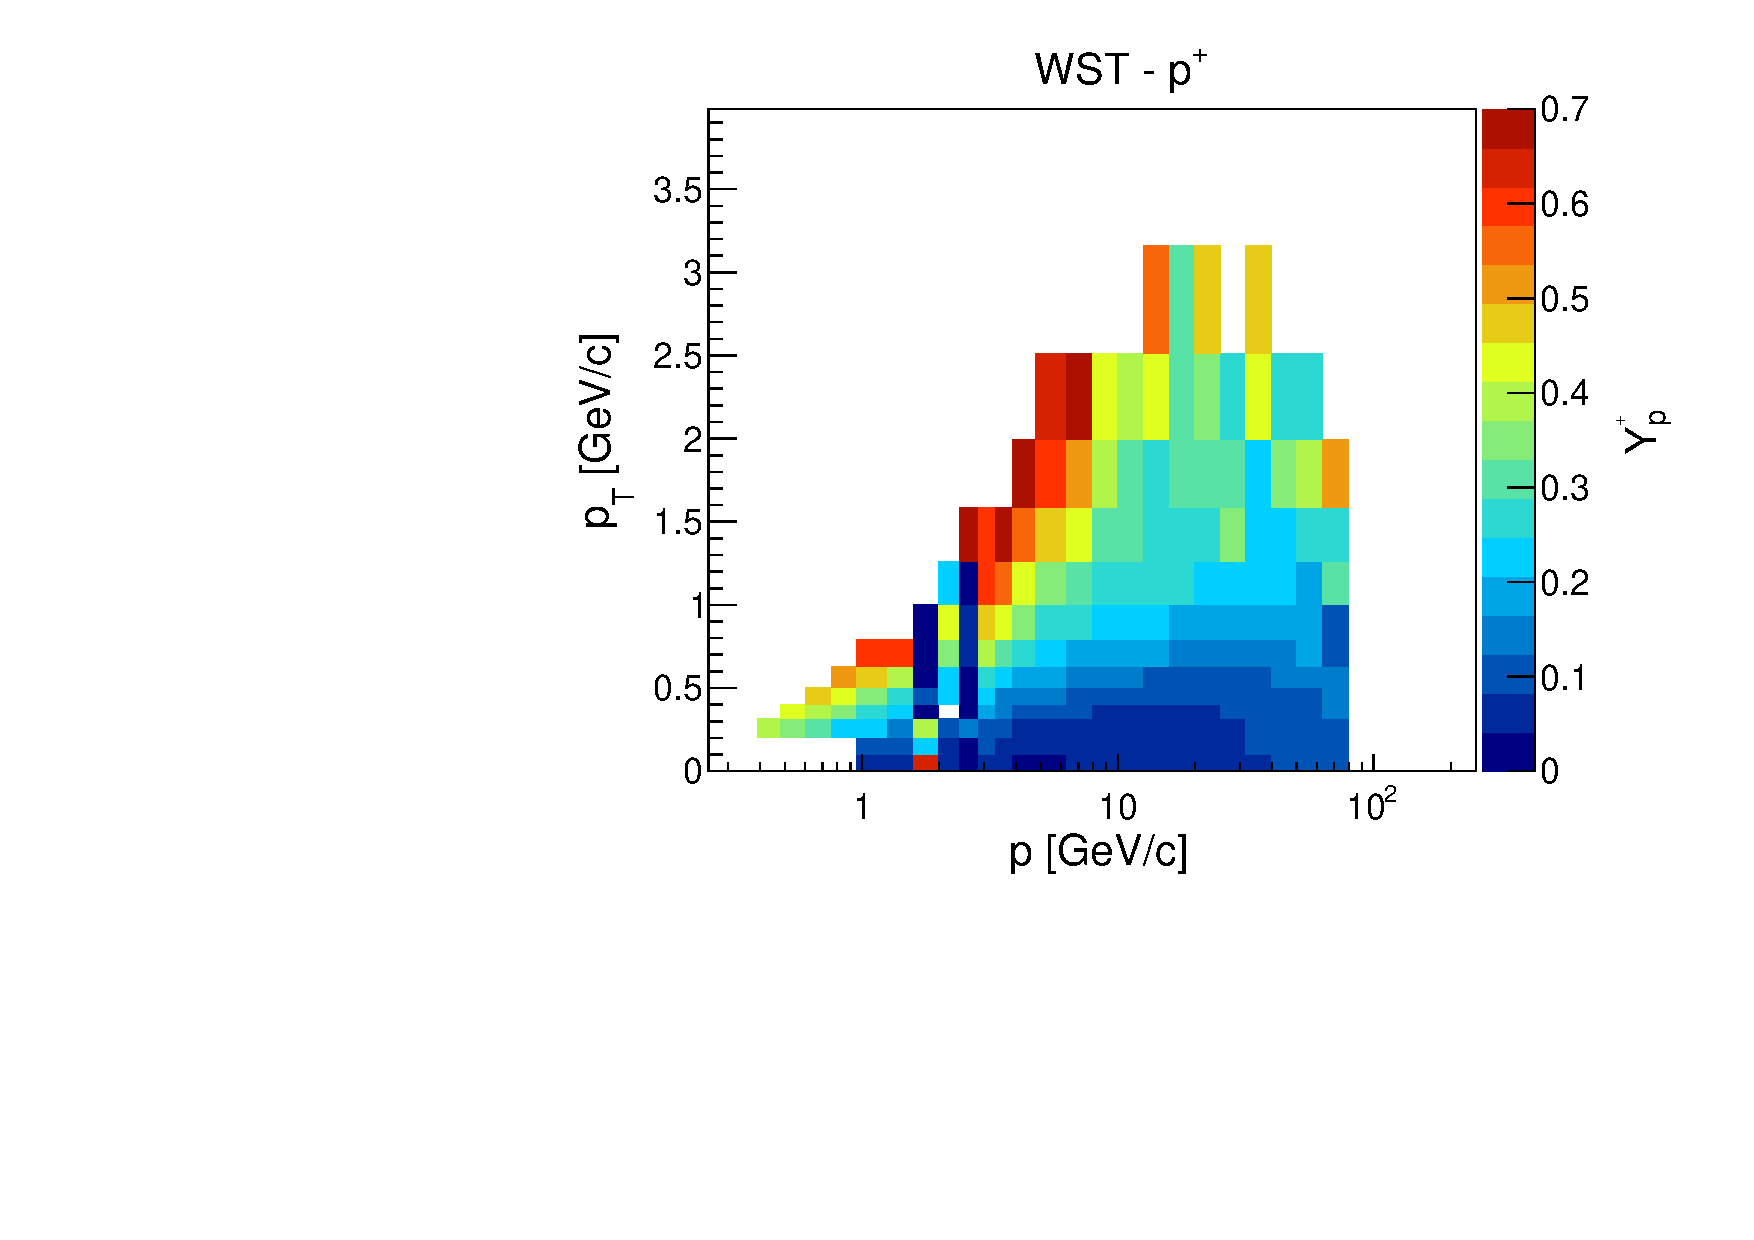
\includegraphics[clip, rviewport=0 0.13 1 0.94,width=0.4\textwidth]{dedx/fraction_158_fl0_v1_c1_p3}

  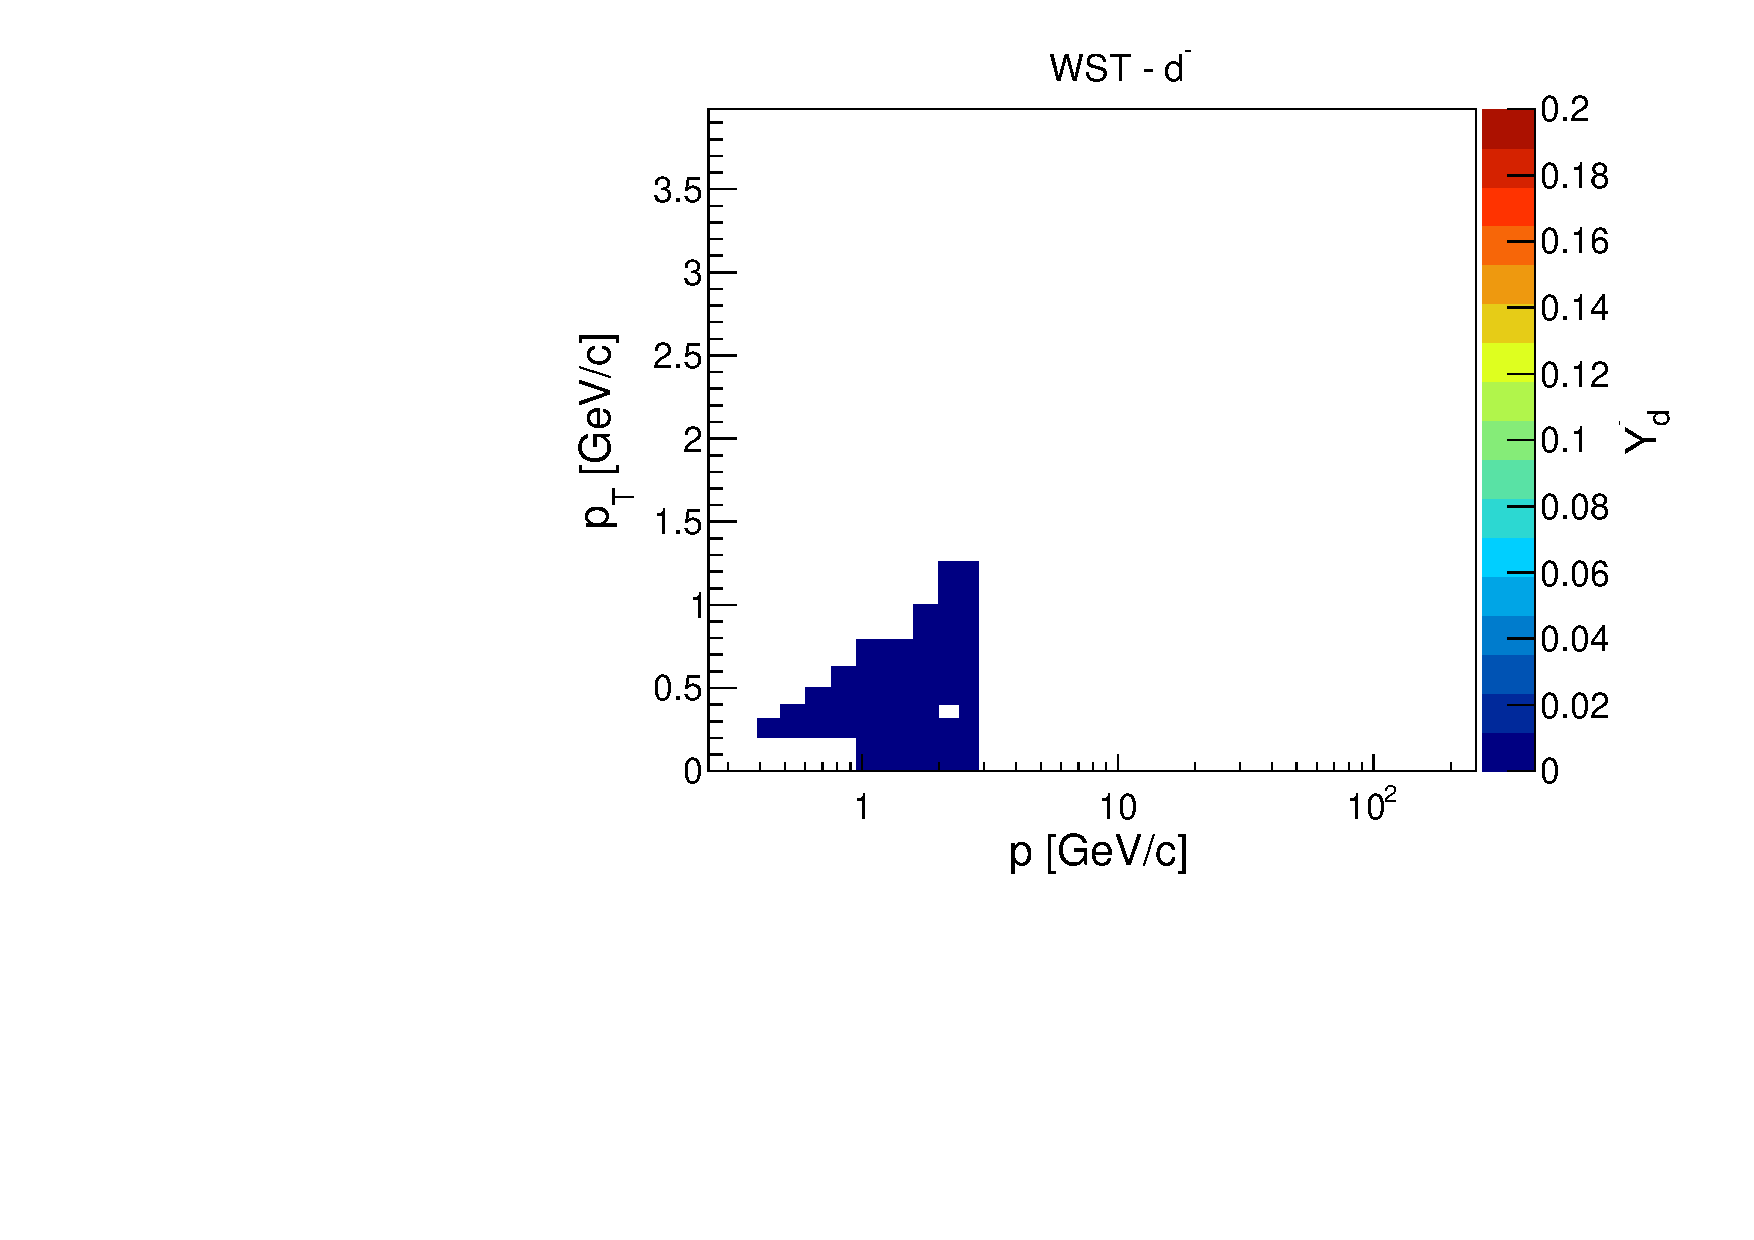
\includegraphics[clip, rviewport=0 0 1 0.94,width=0.4\textwidth]{dedx/fraction_158_fl0_v1_c0_p4}
  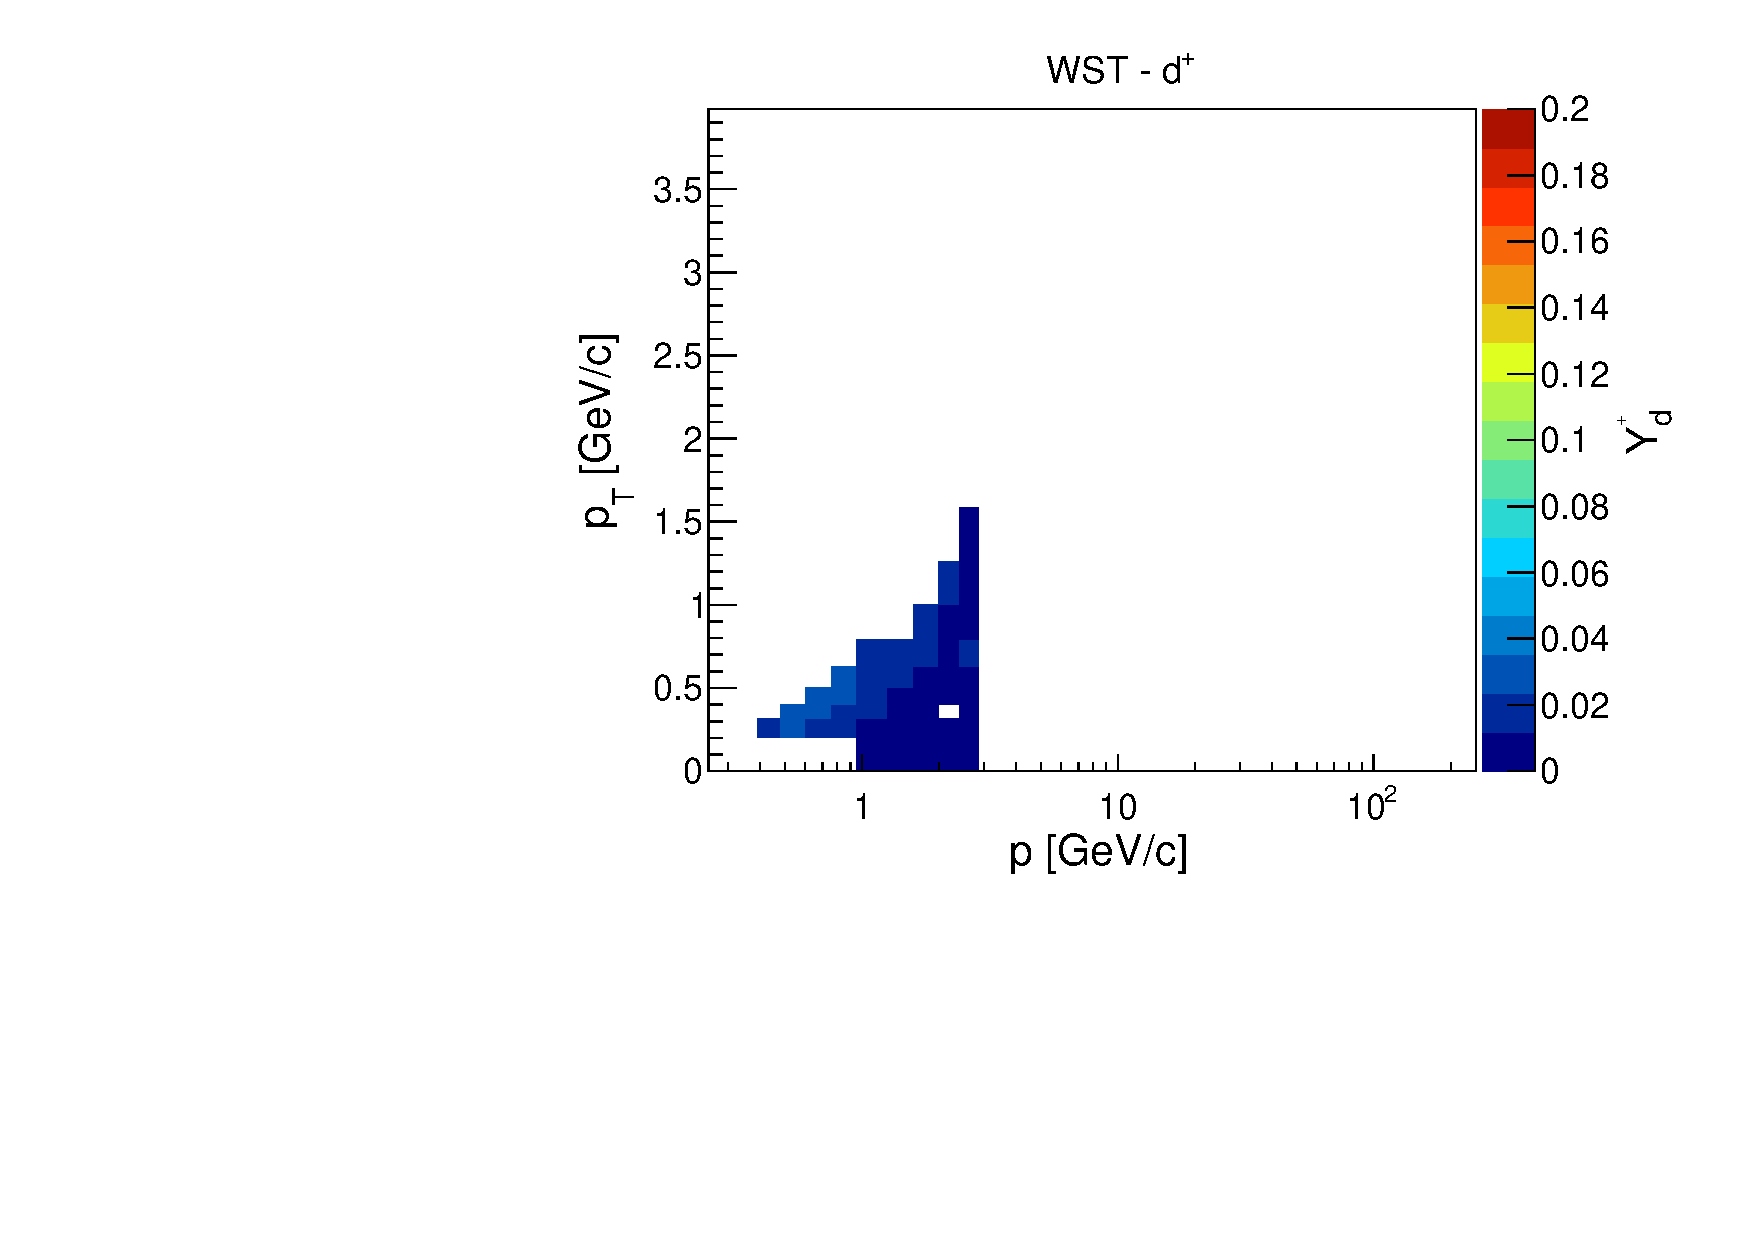
\includegraphics[clip, rviewport=0 0 1 0.94,width=0.4\textwidth]{dedx/fraction_158_fl0_v1_c1_p4}

  \caption{Particle fractions obtained from the fit of the WST dataset at 158 \GeVc.}
  \label{fig:hadron:dedx:fit:frac158w}
\end{figure}


%%%%%%%%%% FRACTIONS %%%%%%%%%%%%%%
\begin{figure}
  \centering
  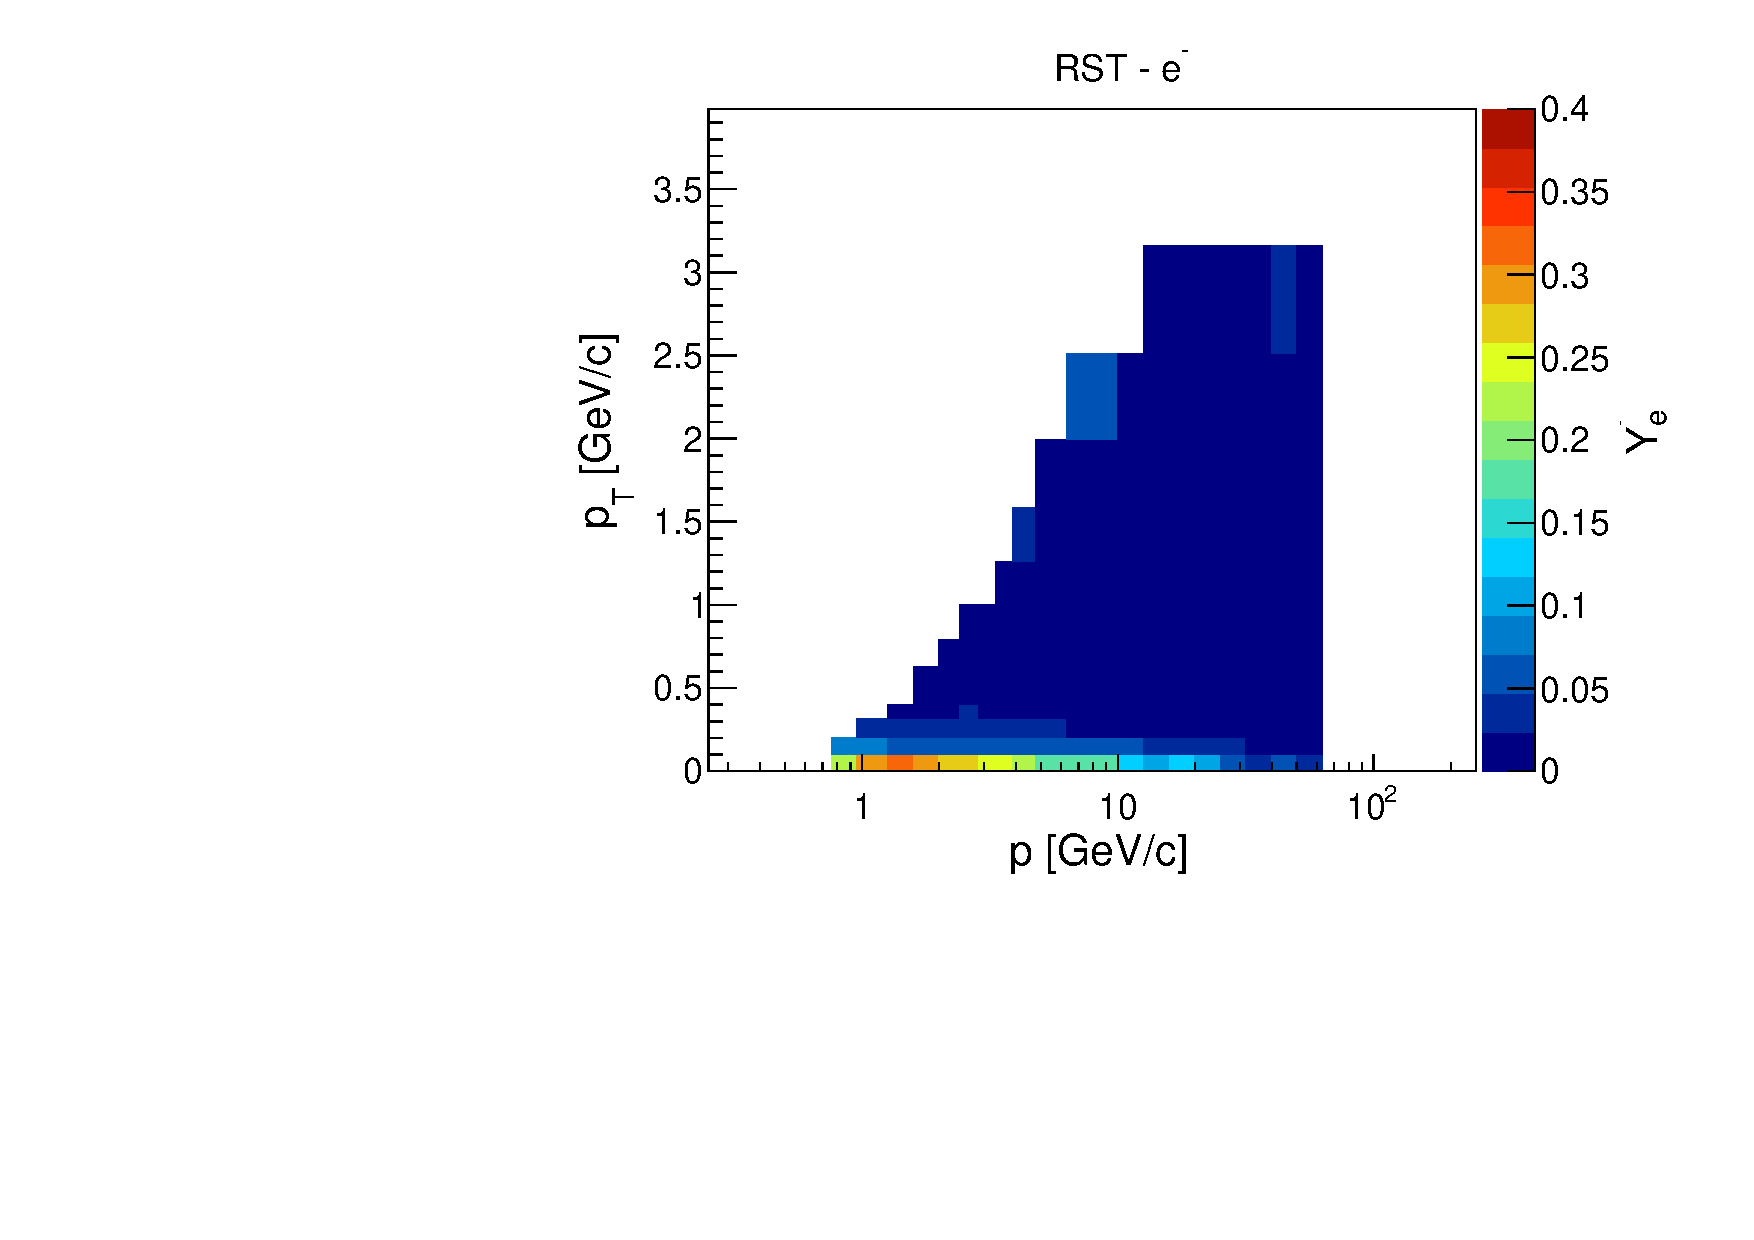
\includegraphics[clip, rviewport=0 0.13 1 0.94,width=0.4\textwidth]{dedx/fraction_350_fl0_v0_c0_p0}
  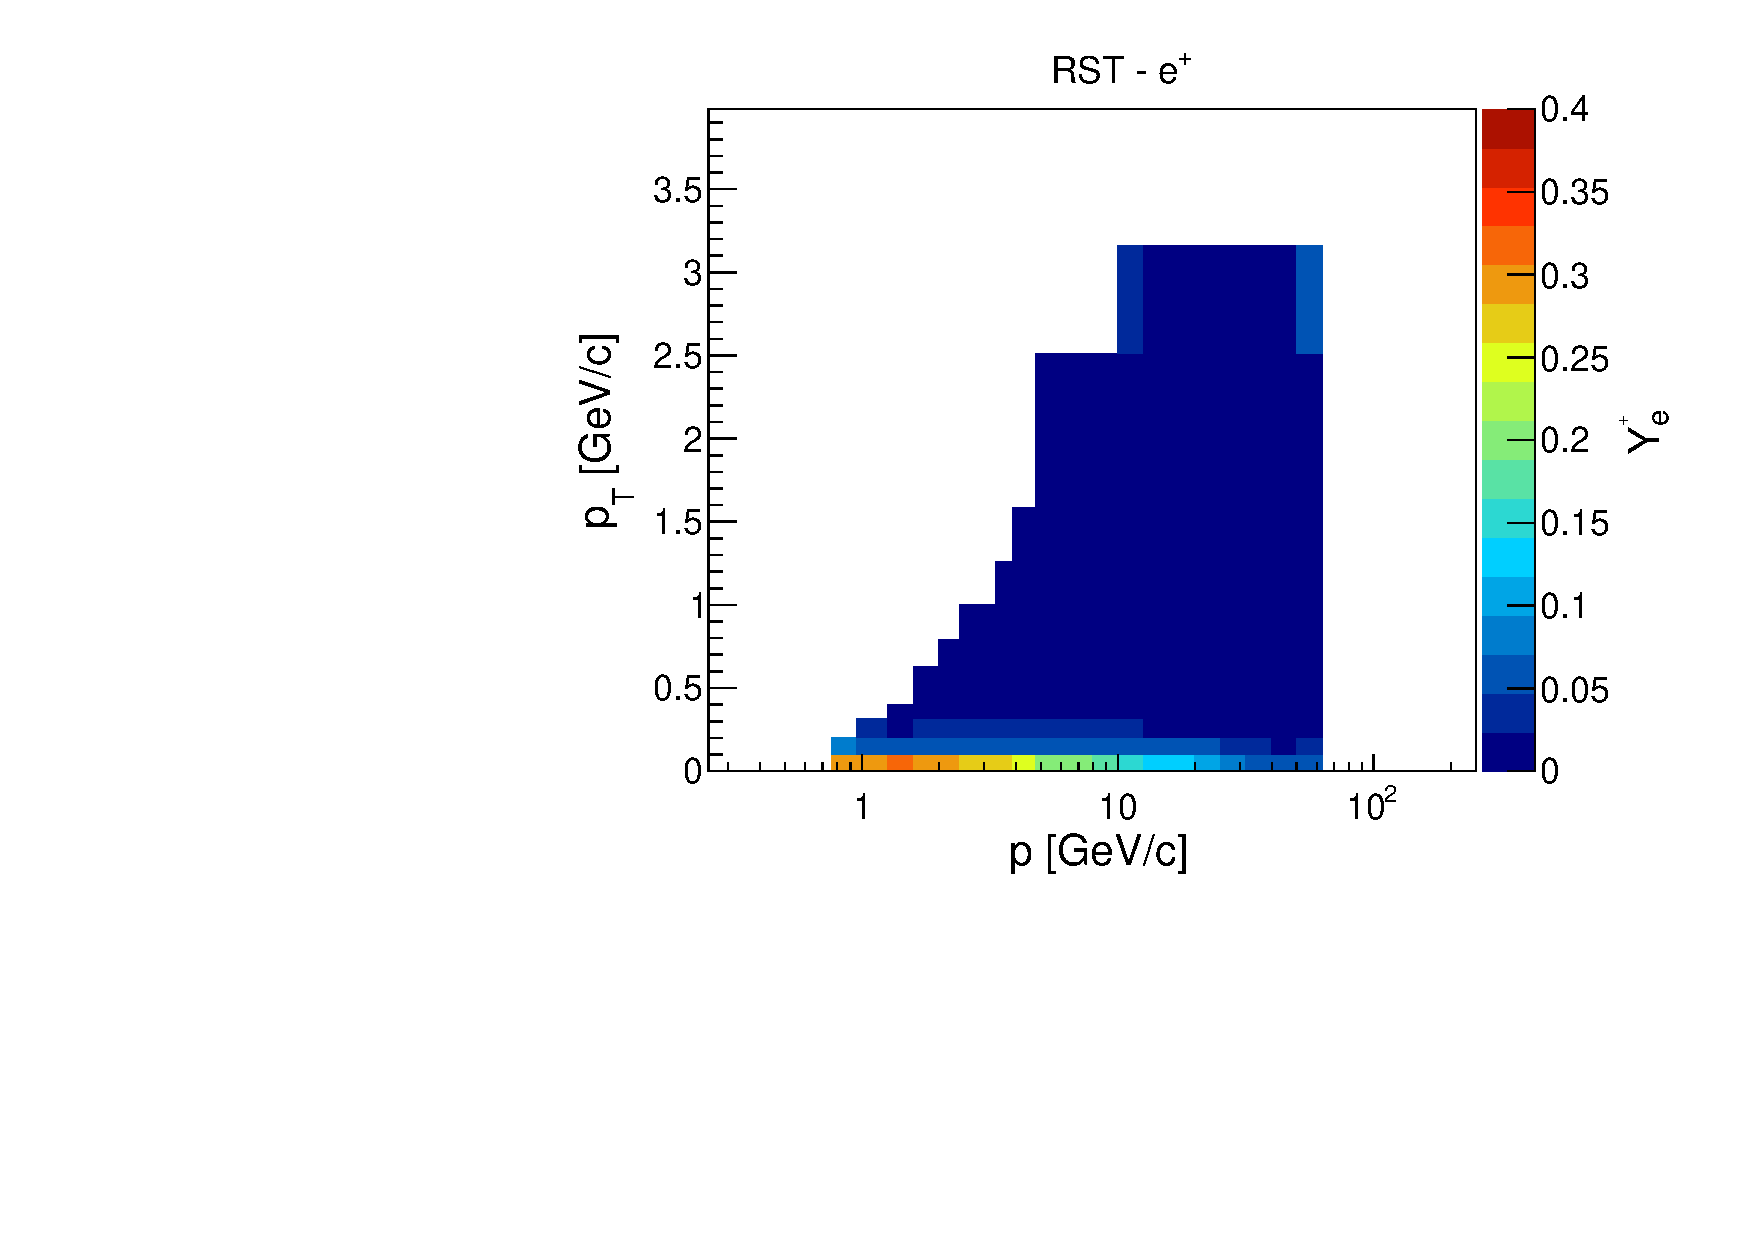
\includegraphics[clip, rviewport=0 0.13 1 0.94,width=0.4\textwidth]{dedx/fraction_350_fl0_v0_c1_p0}

  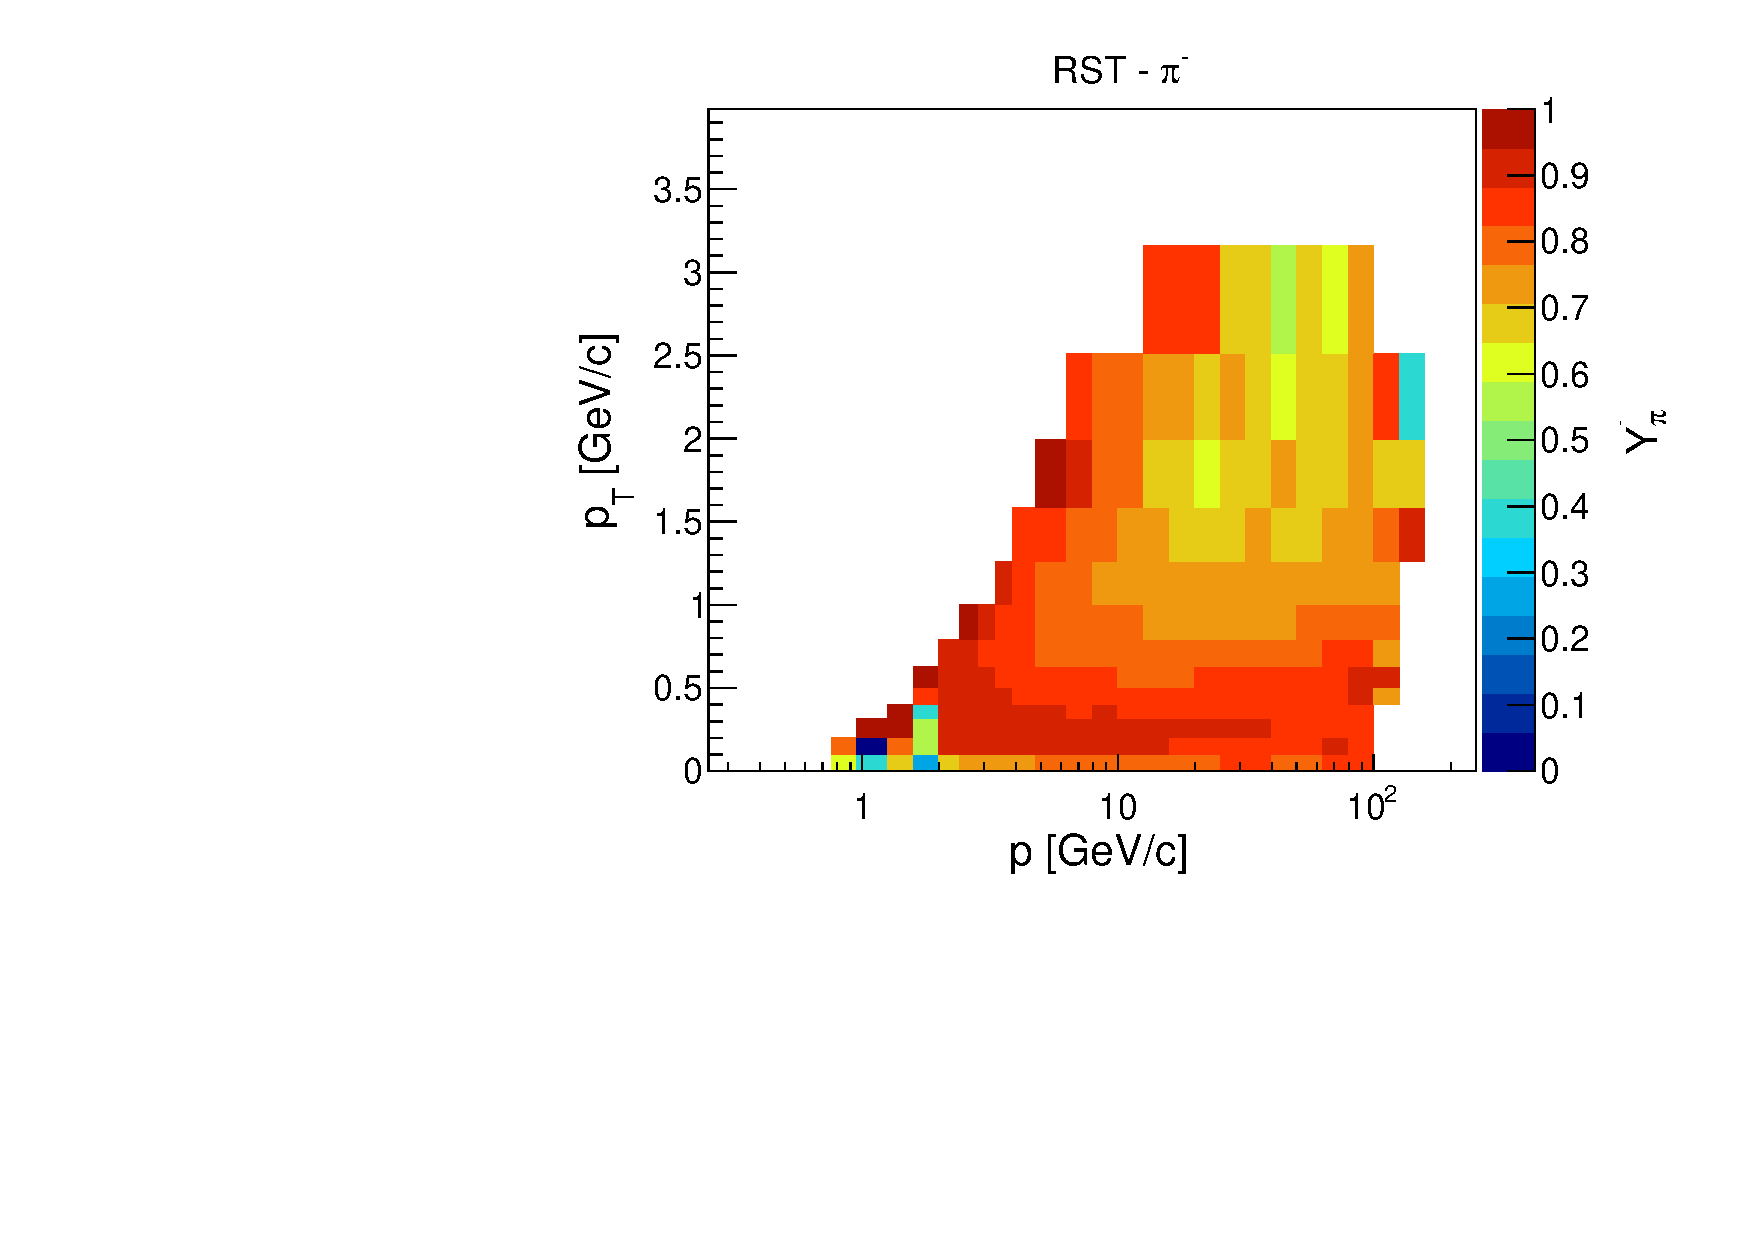
\includegraphics[clip, rviewport=0 0.13 1 0.94,width=0.4\textwidth]{dedx/fraction_350_fl0_v0_c0_p1}
  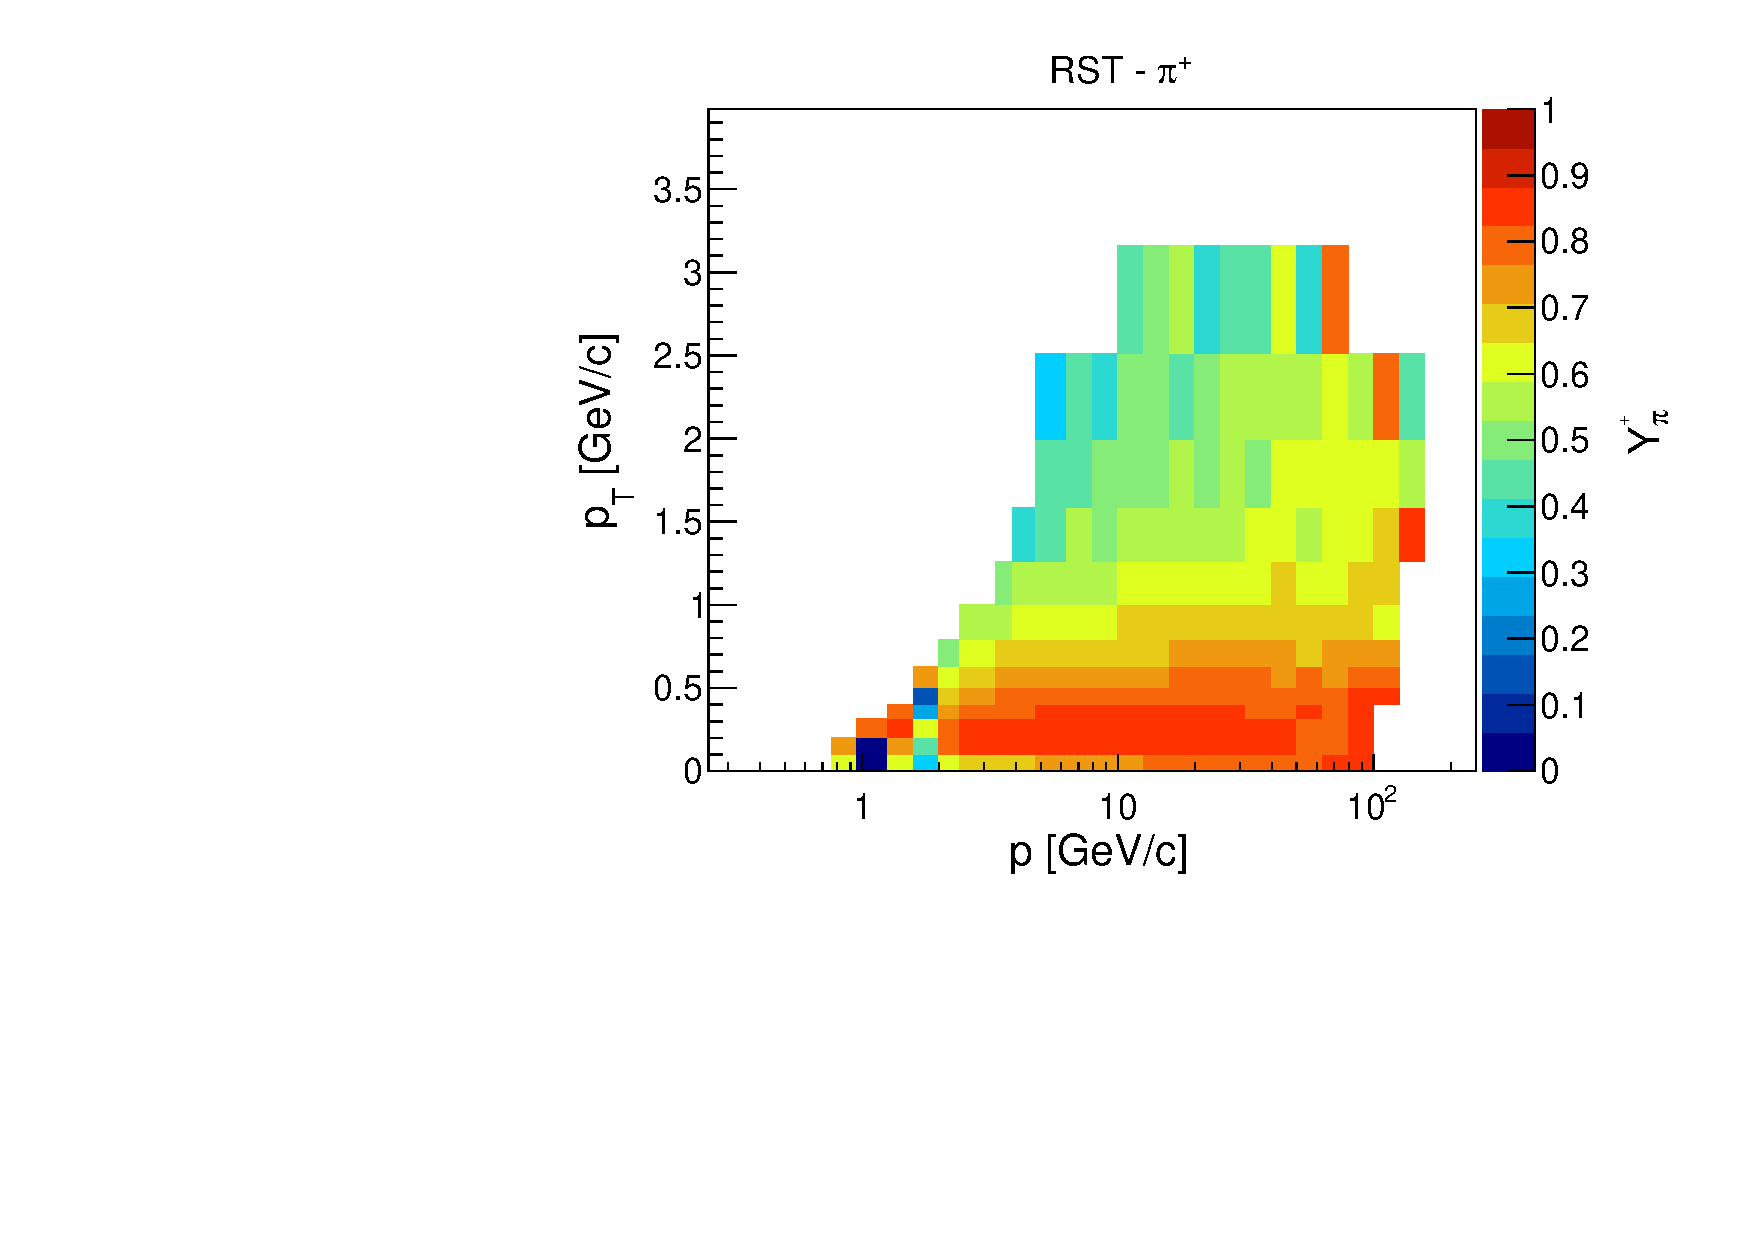
\includegraphics[clip, rviewport=0 0.13 1 0.94,width=0.4\textwidth]{dedx/fraction_350_fl0_v0_c1_p1}

  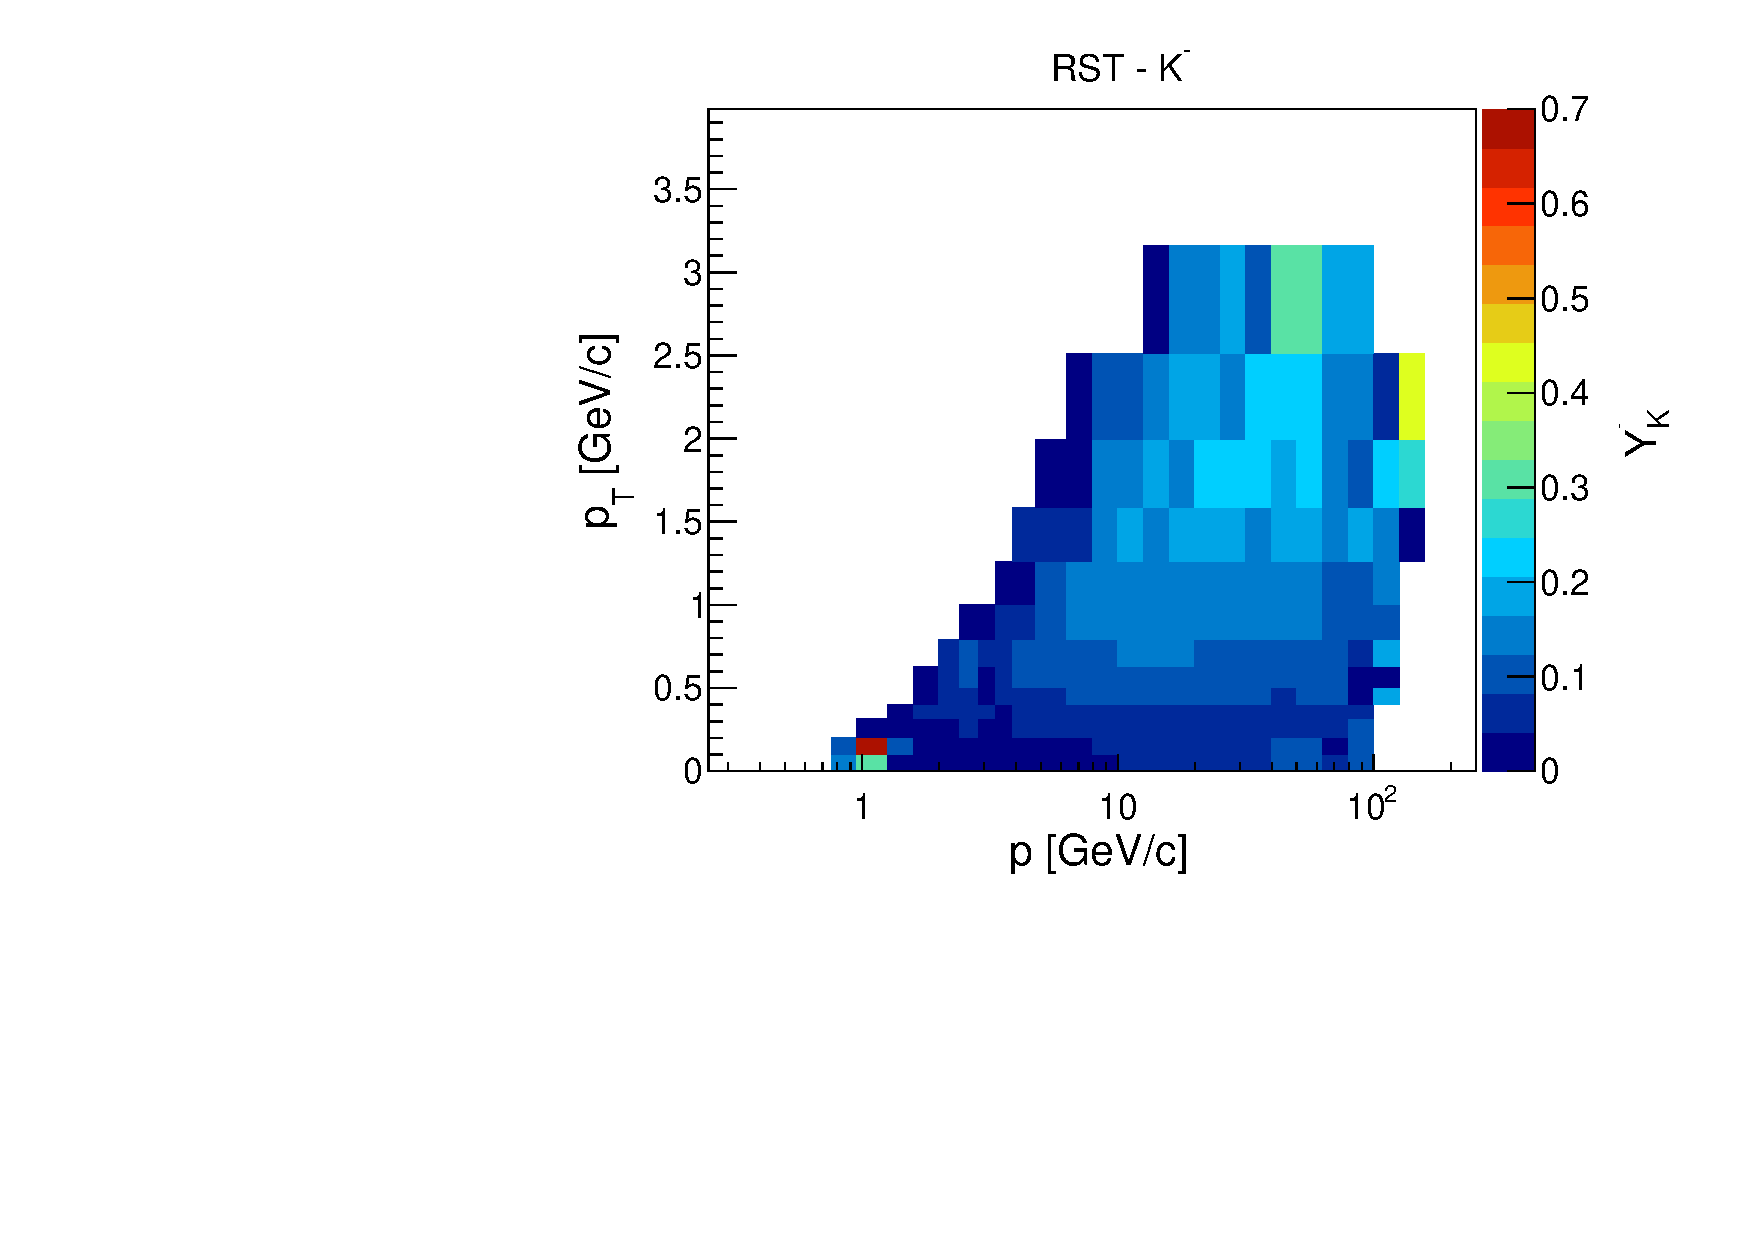
\includegraphics[clip, rviewport=0 0.13 1 0.94,width=0.4\textwidth]{dedx/fraction_350_fl0_v0_c0_p2}
  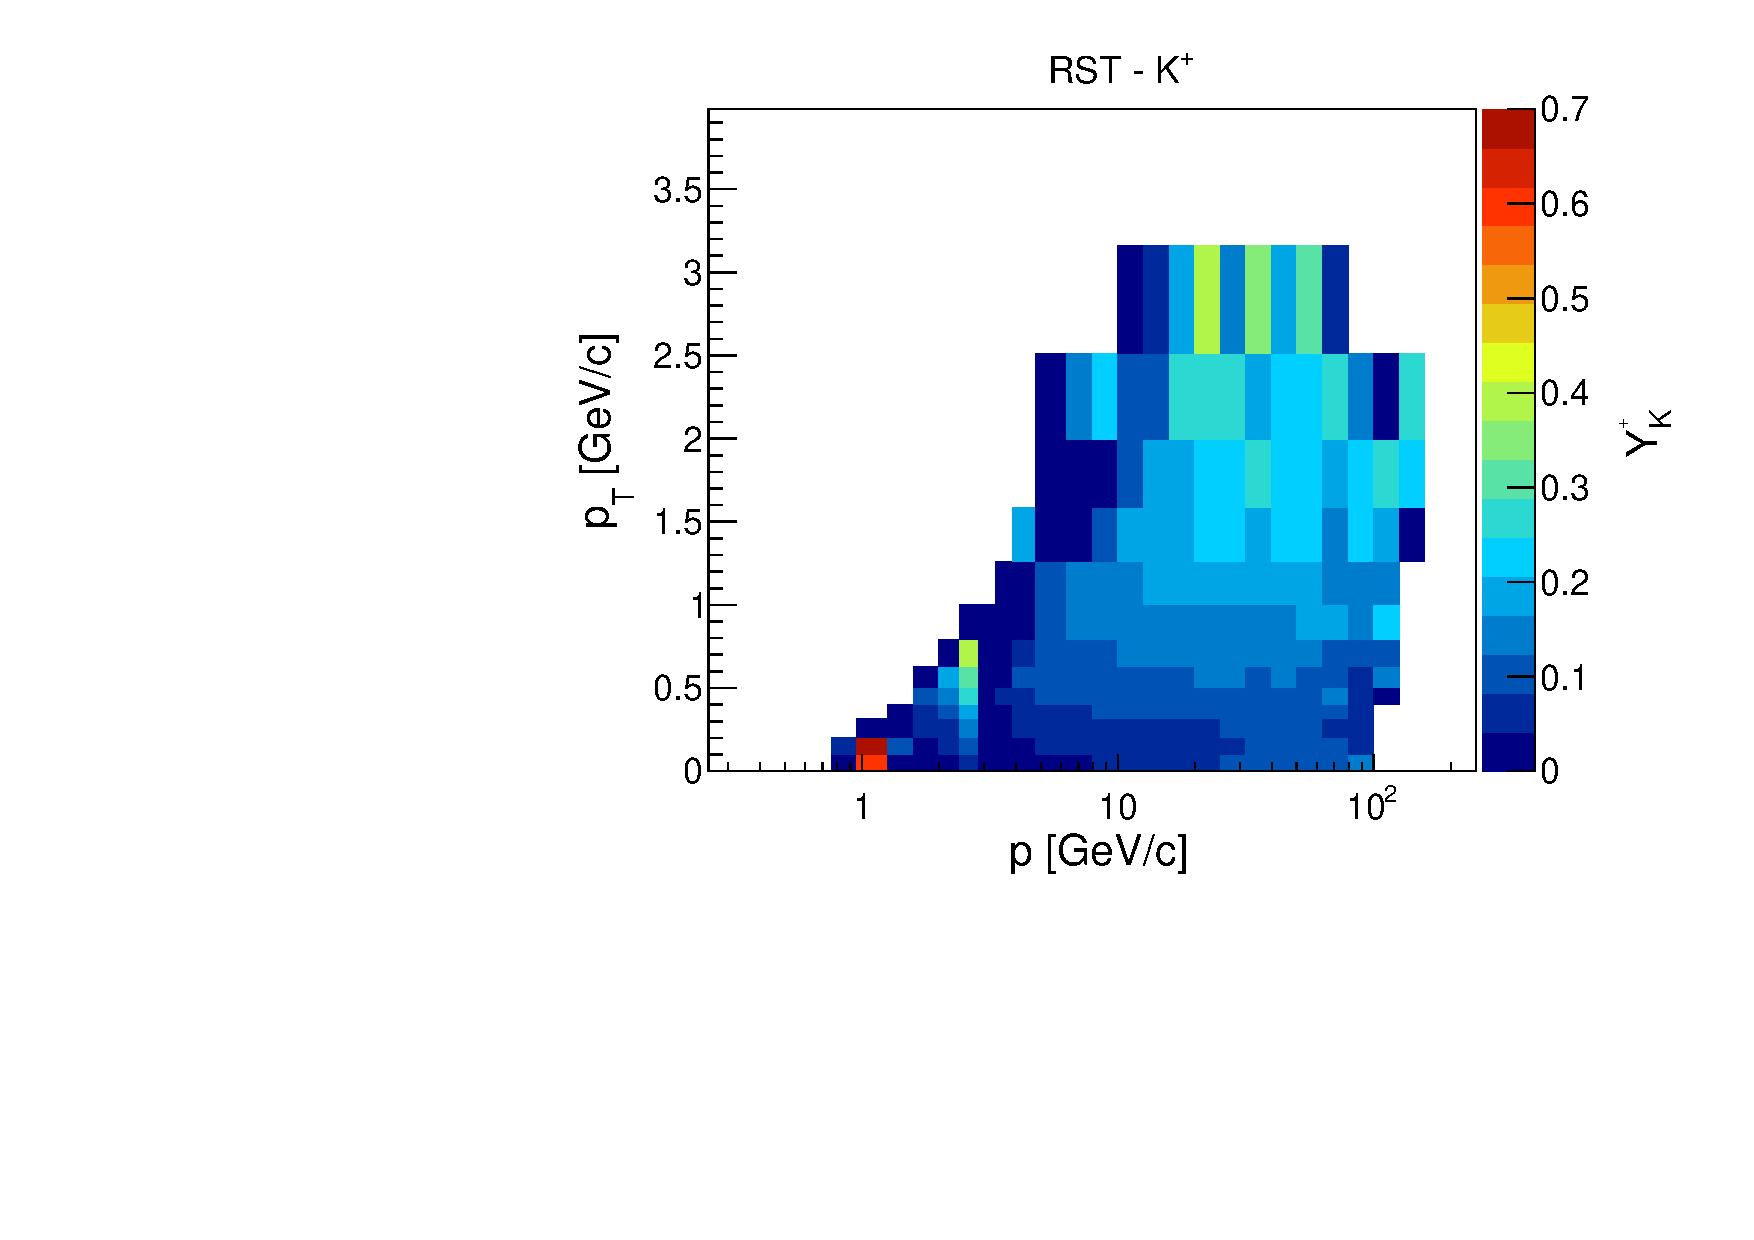
\includegraphics[clip, rviewport=0 0.13 1 0.94,width=0.4\textwidth]{dedx/fraction_350_fl0_v0_c1_p2}


  \includegraphics[clip, rviewport=0 0.13 1 0.94,width=0.4\textwidth]{dedx/fraction_350_fl0_v0_c0_p3}
  \includegraphics[clip, rviewport=0 0.13 1 0.94,width=0.4\textwidth]{dedx/fraction_350_fl0_v0_c1_p3}

  \includegraphics[clip, rviewport=0 0 1 0.94,width=0.4\textwidth]{dedx/fraction_350_fl0_v0_c0_p4}
  \includegraphics[clip, rviewport=0 0 1 0.94,width=0.4\textwidth]{dedx/fraction_350_fl0_v0_c1_p4}

  \caption{Particle fractions obtained from the fit of the RST dataset at 350 \GeVc.}
  \label{fig:hadron:dedx:fit:frac350r}
\end{figure}

%%%%%%%%%% FRACTIONS %%%%%%%%%%%%%%
\begin{figure}
  \centering
  \includegraphics[clip, rviewport=0 0.13 1 0.94,width=0.4\textwidth]{dedx/fraction_350_fl0_v1_c0_p0}
  \includegraphics[clip, rviewport=0 0.13 1 0.94,width=0.4\textwidth]{dedx/fraction_350_fl0_v1_c1_p0}

  \includegraphics[clip, rviewport=0 0.13 1 0.94,width=0.4\textwidth]{dedx/fraction_350_fl0_v1_c0_p1}
  \includegraphics[clip, rviewport=0 0.13 1 0.94,width=0.4\textwidth]{dedx/fraction_350_fl0_v1_c1_p1}

  \includegraphics[clip, rviewport=0 0.13 1 0.94,width=0.4\textwidth]{dedx/fraction_350_fl0_v1_c0_p2}
  \includegraphics[clip, rviewport=0 0.13 1 0.94,width=0.4\textwidth]{dedx/fraction_350_fl0_v1_c1_p2}


  \includegraphics[clip, rviewport=0 0.13 1 0.94,width=0.4\textwidth]{dedx/fraction_350_fl0_v1_c0_p3}
  \includegraphics[clip, rviewport=0 0.13 1 0.94,width=0.4\textwidth]{dedx/fraction_350_fl0_v1_c1_p3}

  \includegraphics[clip, rviewport=0 0 1 0.94,width=0.4\textwidth]{dedx/fraction_350_fl0_v1_c0_p4}
  \includegraphics[clip, rviewport=0 0 1 0.94,width=0.4\textwidth]{dedx/fraction_350_fl0_v1_c1_p4}

  \caption{Particle fractions obtained from the fit of the WST dataset at 350 \GeVc.}
  \label{fig:hadron:dedx:fit:frac350w}
\end{figure}

\clearpage
